%set document properties
\documentclass[12pt, oneside]{report}
\usepackage[utf8]{inputenc}
\usepackage{amsmath}
\usepackage{graphicx}
\usepackage[english]{babel}
\usepackage[a4paper,width=150mm, top=25mm,bottom=25mm, bindingoffset=6mm]{geometry}
\usepackage[table,xcdraw]{xcolor}
\usepackage{booktabs}
\usepackage{cleveref}
%set paths 
\graphicspath{{images/}}

\usepackage{float}
%set citation styles
\usepackage[backend=biber,style=numeric,
citestyle=ieee ]{biblatex}
\addbibresource{ref.bib}

%set headers and footers and import packages
\usepackage{fancyhdr}
\pagestyle{fancy}
\fancyhead{}
\fancyhead[RO,LE]{Analysing the evolution of communication patterns in email data through an extended dynamic network analysis toolkit}
\fancyfoot{}
\fancyfoot[LE,RO]{\thepage}
\fancyfoot[LE,RE]{\thepage}
\fancyfoot[LO,CE]{Chapter \thechapter}
\fancyfoot[CO,LE]{Arshad Ahmed}
\renewcommand{\headrulewidth}{0.4pt}
\renewcommand{\footrulewidth}{0.4pt}
\setlength{\parindent}{0pt}

%packages for captions
\usepackage{caption}
\usepackage{subcaption}
\usepackage{pdfpages}
\usepackage{rotating}
\usepackage{tikz}
\renewcommand*\rmdefault{cmr}
%fixing the spacings
\usepackage{titlesec}
%reduce spacing
%\titlespacing{\section}{1pt}{\parskip}{-\parskip}
%\titlespacing{\subsection}{1pt}{\parskip}{-\parskip}
%\titlespacing{\subsubsection}{0pt}{\parskip}{-\parskip}
\renewcommand\floatpagefraction{.9}
\renewcommand\dblfloatpagefraction{.9} 

% for two column documents
\renewcommand\topfraction{.9}
\renewcommand\dbltopfraction{.9} % for two column documents
\renewcommand\bottomfraction{.9}
\renewcommand\textfraction{.1}   
\setcounter{totalnumber}{50}
\setcounter{topnumber}{50}
\setcounter{bottomnumber}{50}
\usepackage[small,compact]{titlesec}

\date{}

\begin{document}

\begin{titlepage}
    \begin{center}
        \vspace*{1cm}
        
        \huge
        
\includegraphics[width=0.4\textwidth]{city_logo.jpg}
        
        \textbf{MSc Data Science}\\
        \textbf{Project Report}\\
        \textbf{2016}\\
        
        \vspace{0.5cm}
        \Huge
        
        \textbf{\emph{Analysing the evolution of communication patterns in email data through an extended dynamic network analysis toolkit}}
        
        \vspace{1.5cm}
        
        \Huge
        \textbf{Arshad Ahmed}\\
        
        \vspace{1.5cm}
        \vfill
        \Large
        \textbf{
        Supervised by: Dr Cagatay Turkay\\
        Submission Date: 23 September 2016}
       
        
        
    \end{center}
      
\end{titlepage}

\maketitle{}

\chapter*{Declaration}

By submitting this work, I declare that this work is entirely my own except those parts duly identified and referenced in my submission. It complies with any specified word limits and the requirements and regulations detailed in the assessment instructions and any other relevant programme and module documentation. In submitting this work, I acknowledge that I have read and understood the regulations and code regarding academic misconduct, including that relating to plagiarism, as specified in the Programme Handbook. I also acknowledge that this work will be subject to a variety of checks for academic misconduct.  \\


Signed: Arshad Ahmed

\chapter*{Abstract}

Dynamic networks arise in many modern applications such as email, social and telecommunication networks. These networks evolve over time through the addition and deletion of nodes and edges. Thus similarity measures for these networks are critical for us being able to characterise and understand this change. This study explores the use of similarity measures to support dynamic network analysis. To this end we survey existing and proposed methods, apply selected methods to the Enron email dataset and validate against these benchmark measures novel measures introduced in this study. These measures are inspired by the fields of Seismic Data Analysis and Music Information Retrieval. Also we propose novel visualisation techniques to support the analysis of dynamic networks such as the Radon, Frequency-Wavenumber, Audio Waveform and Log Panel Plots. These novel measures are derived using a variety of integral transforms such as the Fourier, Hilbert and Abel transforms. Analysing these attributes derived from the Modularity, Adjacency and Normalised Laplacian graph matrices 
we find that they are best derived from the Normalised Graph Laplacian. To integrate all the existing and novel measures we also propose two aggregation schemes that allow for the derivation of meta attributes such as the RMS and NRMS of the attribute volume derived from the graph time series.  These measures act as effective snapshots of network activity at different time steps.\\

\emph{Keywords:} Dynamic Network Analysis, Attribute Analysis, Multi-Attribute Visualisation

\tableofcontents

\listoffigures

\chapter{Introduction}

\section{Background}
Networks arise in many modern day applications such as email, social, transport and telecommunication applications. These networks represent convenient structures to analyse phenomenon that would be very difficult to analyse otherwise. However, with most modern networks a key feature is that these networks evolve over time. These dynamic networks require analytical methods that would allow easy comparison between them at the different time steps. Thus similarity measures that allow us to assess and track change over time in such networks are instrumental for us to be able to study such networks. Therefore similarity analysis on dynamic networks is of critical importance if we are to be able to understand this evolution over time. This study is motivated by the need to explore the effectiveness of traditional Network Analysis metrics such as centrality analysis in the context of dynamic networks in addition to exploring novel measures. \\

The traditional metrics were developed mainly for the analysis of static graphs thus for modern applications their suitability needs to be assessed and their shortcomings determined. In this study we find that although these measures can be utilised in a dynamic network context they are useful for benchmarking of other new measures.
The field of Dynamic Network Analysis spawned with the explicit aim of expanding our toolkit to handle such complex evolving networks.  \\

In this study we propose novel measures of similarity which are motivated by the fields of Seismic Data Analysis and Music information Retrieval. These novel measures proposed here are calculated from the Normalised Graph Laplacian. Some of these new attributes behave very similarly to traditional centrality measures while being sensitive to smaller changes in the network that traditional measures do not pick up on as well. \\

In addition to capturing network dynamics we show that by utilising such attributes some aggregated network measures such as Average Degree could be predicted with a good level of accuracy using a Gradient Boosting Regression Technique. This is useful because having metrics that allow us to potentially model the change of the network under consideration can help us understand the key drivers even better. For example this method enables feature ranking of attributes in this data the attribute derived from the Abel Transform is found to be particularly useful. This is interesting because this attribute appears to capture hidden dynamics which become apparent through mapping to these alternative spaces but the traditional metrics do not feature highly on this list. So there is a case for these attributes to be used in a predictive context. \\

This study also introduces a number of visualisation techniques to support the joint analysis of these attributes. These are namely the Radon, Frequency-Wavenumber (FK), Log Panel and Audio Waveform Plot. The Radon and FK  plot serve as a form of dimensionality reduction and allow us to visualise the whole derived attribute volume in these alternative spaces in 2 dimensions. The Log Panel allows the analysis of multiple attributes by placing them along panels side by side. These can be arranged in a number of ways such as the attributes can be grouped by type such as Centrality measures, Seismic and Music attributes or they can be sorted by cluster indices from a hierarchical clustering procedure. This name is inspired by Well Log Panels which are used in hydrocarbon exploration to help map lithologies using a variety of logs captured while drilling.

\section{Paradigms of Network Analysis}

The literature suggests 3 main paradigms of network analysis these inform the framing of research questions and investigative approach. These can be broadly described as: \cite{Chapanond2005}

\begin{itemize}
    \item Social Network Analysis (SNA)
    \item Dynamic Network Analysis (DNA
    \item Supernetwork Analysis (SuNA)
\end{itemize}

\subsection{Social Network Analysis (SNA)}

SNA is concerned with the study of relationships between entities and its focus of research is of two types: whole network analysis and self-centred network analysis. Whole network analysis is concerned with understanding the structure of relationships between different roles in a group and is used to investigate network structure changes with the time and the contact pattern of network entities. Self-cantered network analysis is concerned with how the individual behaviour of network entities are influenced by the membership of the network. \cite{Chapanond2005}

\subsection{Dynamic Network Analysis (DNA)}

DNA was proposed as an extension to the SNA. The strength of DNA is that it is able to handle large scale dynamic, multi-modal, multi-lateral network with various levels of uncertainty. The edges are probabilistic and the nodes behave like agents in a multi agent environment so this enables perturbations or changes in the network to propagate through the network and result in some global reconfiguration. The evolution of a network in The application of machine learning and multi agent modelling in the same environment is enabled by DNA’s use of the meta matrix.\cite{Chapanond2005} 

\subsection{Super Networks Analysis (SuNA)}

Super networks can be thought of as networks of networks that exist above and beyond existing networks. These have the characteristic of being multi-layered, multi-dimensional, multi-attributed and multi-levelled with additional features such as congestion and coordination. These have been applied predominantly in supply chain management, finance, traffic and ecology among others. These networks are analysed using either variational inequality and/or hyper graph theory. \cite{Chapanond2005}

\section{Recent Work}

\citeauthor{Li2016}\cite{Li2016} notes the complexity and difficulty of Dynamic Network Analysis as a field of study. They note that modern applications such as the Internet of Things and mobile social networks we are faced with networks that are not only large but having complex dynamics associated with them. This is driven by the fact that node numbers and connections grow exponentially with connections constantly being added and broken. The properties of these networks evolve with time. This is the defining feature of a Dynamic Network. They are characterised by their time dependent topology due to fluctuations in the underlying network activity. As traditional data mining techniques are deemed to computationally expensive or insufficient when faced with such complex networks they suggest a visualisation based method in which the links in the dynamic graph are broken down by the time dimension. Each segment as a result represents a time step of the evolution of some property of the dynamic network. The key contribution is that their approach is a static view based approach which does not require the end user to have a mental map of the previous steps to enable analysis as in animation based methods. As a result it is easier for the end user to detect patterns and identify potential anomalies.\\

\citeauthor{Pereira2016}\cite{Pereira2016} introduce the notion of evolving centralities in temporal networks in the context of social networks. They analyse data from Twitter but in order to understand the reaction of the structural position of the user with the underlying network evolution they utilise follower/followee networks are analyse the centrality evolution over time. Their approach is different in the sense that their approach is based on temporal graph theory. This enables more sophisticated analysis as the shortest path can be interpreted as a function of time and therefore they are able to recalculate the closeness and betweenness centrality using these fastest paths. This leads to their insight that Twitter users are dynamic and can assume or leave central positions in a network. \\

\citeauthor{Wu2015}\cite{Wu2015} propose a graph based decay function to update the frequency of user interactions in a social network and then use a community detection algorithm to detect communities at each time step. They find that most studies ignore the temporal information in the study of community structure in networks and show that by incorporating such information is very helpful in the analysis of community evolution analysis in social networks.\\

\citeauthor{Hu2015}\cite{Hu2015} use probabilistic graphic models to detect time-evolving influence among objects from dynamic heterogeneous graphs. They note that the dynamic nature of such heterogeneous graphs where nodes and edges are added or removed dynamically are not sufficiently addressed by current studies. Therefore to handle the dynamics of the network and to learn the time evolving influence structure they propose to use probabilistic graphic models using the graphs at discrete time stamps. \\

\citeauthor{Mahyari2015}\cite{Mahyari2015} discuss signal processing on graphs and introduce the Fourier Transform for dynamic networks. They do this by finding a common subspace across a modified common Laplacian matrix for the dynamic networks. The eigenvectors of this Laplacian form the Fourier basis for the networks. From this common subspace the eigenvalues correspond to frequency components. Therefore high eigenvalues correspond to high frequency and vice versa. The Fourier transform is used extensively in this study for the derivation of the multiple attributes and supports many visualisation techniques as will be discussed in Chapter 3.  The key difference between this study and our work is that they first find a subspace and then find the Fourier Transform of it and we apply the integral transform directly to the matrix and derive attributes from Fourier space.\\

\citeauthor{Lansing2016}\cite{Lansing2016} propose to assess the temporal evolution of networks by first transforming networks into signals through Classical Multidimensional  Scaling  based  on  the  resistance  distance  and then constructing  a  tensor  based  on  the  spectra  of  each  signal  across time. We use the average resistance distance as an attribute to map change in the graph time series. Also we use Non-metric Multi Dimensional Scaling to visualise the relationship between the attributes.

\section{Motivations and Aims}

From the brief overview presented above it is clear that a lot effort and attention has been given to the topic of dynamic network analysis. These papers touch on various methods that we use in our study. But the wide variety of our methods and the nature of our application to dynamic networks to the best of our knowledge is unique and not encountered in the literature. \\

By treating the dynamic network as a time series we characterise each point in the series of the graphs by a number of attributes. These serve as a compact feature based representation of the network. The attributes are then collapsed into a single value either by taking the average or the Frobenius Norm where appropriate. \\

This is done for traditional centrality measures as well as the novel metrics. We show that by directly applying the integral transform to the Normalised Graph Laplacian there is no requirement to find a common subspace first. The application gives us a common subspace in the alternative space such as Fourier, Hilbert and Abel etc. We can then efficiently calculate multiple attributes in these spaces which can then be compared over the time range in question. \\

Also the treatment of networks as a music signal is novel. This approach opens the doors for many methods from digital music to be applied to networks. Therefore we can confidently state that we are addressing a real need for metrics designed to capture dynamism in networks. As a result we open the doors to many more methods to be imported not just from the fields from which we take inspiration but from other fields which use similar techniques. \\

The Fourier Transform forms the basis of many techniques explored in this study. However, in contrast to this work where the authors try to characterise the change in the spectral content of a common Laplacian. We in this study show that by using the Normalised Graph Laplacian we are able to derive a frequency representation for the graph time series. From the frequency of the individual graphs we can derive attributes such as the Norm of the Abel transform of the magnitude of the Fourier Spectrum for the dynamic network. \\

As mentioned that the analysis of dynamic networks is necessitated by the need to understand and model complex phenomenon. Undoubtedly there is great value in understanding the dynamics of such networks. The beneficiaries of this work are practitioners who are interested in or need to study dynamic networks. These could range from intelligence agencies monitoring changes in terrorist networks, social media companies monitoring and understanding the dynamics of their networks to telecommunications companies trying to identify interesting network dynamics that can drive their business forward. \\

The main aim of this study is to explore these metrics using the Enron Email Network Data. This will serve as a proof of concept for these attributes and visualisation techniques as well as outline a generalised work flow for the systematic robust analysis of dynamic networks. \\

A evaluation strategy is highlighted in this strategy that allows for a logical exploration and validation of these attributes and can serve as a road map for future work in this area.  \\

Underlying all these analysis is the fact that these measures serve as a snapshot of a network at a point in this time. Thus sampling these measures at the different time intervals it is possible to derive a time series of attributes from the graph time series. This time series approach allows utilisation of methods from signal processing because by treating the graphs at the different time steps as a time series and the derived attributes also as a time series we can apply methods from signal processing \\

From the field of Seismic Data Analysis we present a number of attributes which are based on the notion of the Complex Trace. This involves using the Hilbert Transform and using the Real and Imaginary components to derive attributes such as Amplitude, Phase and Frequency. From this a number of other attributes are derived. wen addition matrix decomposition methods such as Kernel Principal Components Analysis (KPCA) and Non-negative Matrix Factorisation (NMF) are used to derive additional measures. \\

From the field of Music Information Retrieval we implement two measures the Zero Crossing Rate and the Spectral Centroid. This is possible by treating the networks as a audio signal by the use of the Fourier Transform on the Normalised Graph Laplacian. \\

Both sets of similarity measures that we will call Seismic and Music attributes for convenience are well established in their respective but their application to dynamic networks is novel. The motivation to utilise these measures is driven by the need to have measures that are scalable, have a relatable interpretation and are particularly suited for dynamic analysis. For example the seismic attributes are commonly analysed for the identification of hydrocarbon reservoirs and in 4D seismic two surveys are compared at different time steps to characterise change as a result of production from a field. So these measures become particularly suited for analysis with a time component. \\

Therefore the key motivations for this project can be summarised as firstly to develop an understanding of the use of traditional metrics to define a signal in a graph time series. Secondly, to complement existing measures with novel ones which will enhance our analytical capabilities for the structure of dynamic graphs. Third, to develop visualisation techniques to enable multiple attribute analysis and finally aggregation measures which can serve as a proxy for network activity. \\

\section{Beneficiaries}
Although the analysis presented in this study uses an email network the methods proposed here are generalisable to any dynamic or static network. This is because the attributes are calculated from the matrix of the graph structure like the Normalised Graph Laplacian. Therefore any problem that can be modelled as a network can be expressed as a Normalised Laplacian Matrix and these attributes can be easily calculated from it. This opens up these methods to practitioners and analysts from a wide variety of fields as a result.\\

The main beneficiaries are practitioners or analysts who are involved or have an interest in the study of dynamic networks. This can range from social media companies trying to understand structural changes in their network and being able to identify easily the key players. wet could be useful to intelligence agencies analysing threat networks they have more tools to characterise the structural change in networks and identify times and nodes of interest. wet could also benefit telecommunications companies from example to understand how fast their network is expanding or contracting and more importantly predict some fundamental network property such as Average Degree at a time step in the future. Understanding potential trends in advance has the capacity to drive changes in strategy, enhance planning and deliver increased value for the business. 

\section{Objectives}
The objectives that will help us answer our research question are as follows:

\begin{itemize}
    \item Explore similarity measures proposed for the analysis of networks
    \item Explore the use of these measures in a practical context
    \item Evaluate how such measures can be applied to the analysis of dynamic networks and develop a generalised work flow
    \item Derive novel attributes based on signal processing type approaches and benchmark their behaviour against existing measures
    \item Develop visualisation techniques to support multiple attribute analysis on dynamic networks
    \item Suggest aggregation schemes to serve as a snapshot of network activity over time
\end{itemize}

\section{Research Question}

The research question can be stated formally as follows:\\

\emph{How can similarity measures be used to analyse dynamic email networks? How can similarity measures in alternative spaces support the analysis of dynamic networks?}

\section{Overview of Methodology}

The methodology followed in this study is as follows:

\begin{enumerate}
    \item Source an appropriate email network network dataset with timestamps 
    \item Break data into yearly and monthly sets with no temporal aggregation
    \item For the graph time series at the monthly and yearly level analyse the networks through traditional measures such as Centrality, Algebraic Connectivity, Density and Average Clustering Coefficient. These form the benchmark measures against which other measures are compared.
    \item For the novel measures proposed determine which of the 3 graph matrices:  Modularity, Adjacency and Normalised Laplacian yield the most stable attributes. This is done by analysis of the Signal to Noise Ratio, Mean Absolute Deviation, numerical magnitude of the attributes and their ability to model the signal in the benchmark measures. 
    \item Pick the Matrix yielding the most stable attributes using this to explore correlation among the measures, new visualisation approaches and aggregation schemes.
    \item Scale all attributes to [-1,1] interval for comparability.
    \item Perform correlation, regression and manifold reduction analysis to understand the relationship between all the different attributes
    \item Derive node level trends for common nodes at the yearly level for centrality measures
    \item Explain trends in the yearly and monthly trends relating to network visualisations while evaluating the ability of the measures to represent the graph time series signal
\end{enumerate}

\section{Report Structure}

This report is structured into 6 key chapters. The in Chapter 1, the main aims, motivations, objectives and research questions are stated for clarity and final evaluation of the outcomes. In Chapter 2, we present a literature review where all the relevant information is summarised and presented. This serves to inform the rest of the analysis conducted. The analytical methods are presented in detail in Chapter 3. Chapter 4, shows all the results due to the applications of the measures in Chapter 3. We also present a detailed discussion noting our observations on structures and trends from the data. Chapter 5, presents a detailed evaluation of the methods and we answer the research question that we stated in Chapter 1. Chapter 6, concludes with our reflections, suggestions for further work and final conclusions of this study. 



 







\chapter{Critical Context}

\section{Graph Terminology}
The origins of graphs theory can be traced back to Leonhard Euler and his approach to solving the Konigsberg Bridge Problem. This city was located on the Pregel River in Prussia. The river divided this city into 4 distinct areas which included an island all of which were connected by a total of 7 bridges. Euler’s representation of this problem of the individual areas as nodes and the bridges as edges is considered one of the first applications of graph theory.\cite{Dickson2006}

\begin{figure}[h]
    \centering
    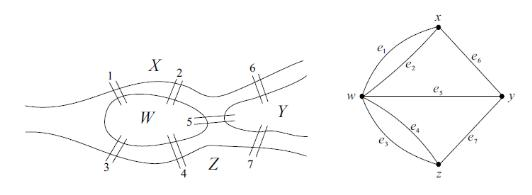
\includegraphics{euler}
    \caption{Euler’s graphical representation of the Konigsberg Bridge Problem.}
    \label{fig:Konigsberg Bridge Problem.}
\end{figure}

\\
A graph, G can be described as a triple which consists of a set of edges E (G), a set of vertices or nodes V (G) and a relationship that connects the vertices to these edges. Finite graphs are those that have V and E as a finite set. Simple graphs are those that have no loops or multiple edges. A path is simple graph in which the vertices can be ordered where two vertices can be adjacent only if they are consecutively ordered. A cycle is defined as a simple graph where the vertices can be cyclically ordered such that two vertices are adjacent only if they are consecutive in cyclical ordering. A subgraph can be thought of cycles and paths within a larger graph, where the edge relations between the subgraph and the large graph are the same. \cite{Dickson2006}\\

\section{The Limitations of traditional SNA}

In Social Network Analysis (SNA), traditionally bounded networks are considered with maybe 2 or 3 connection or link types such as friendship or advice between a node types such as people sometimes another node type such as events are also considered together. \cite{Carley2001}\\

If we consider more critically the interactions possible within our problem context of email networks we can have email networks within an organisation which are bounded and also with other organisations, clients and stakeholders and then the network does become unbounded. These networks can then be thought of as a higher order networks and as  \citeauthor{Carley2001}\cite{Carley2001} notes many tools developed for simpler networks do not scale well to increased network size and complexity and in some cases experience degradation through increased susceptibility to Type 1 and Type 2 errors. \\

The dynamics in these networks can arise from different processes depending on the context of the problem. Natural evolutionary processes would be learning, births, deaths and ageing Others could be as a result of intervention measures such removal or addition of nodes i.e. removing those who lead the system, communities forming or disintegrating. The data associated with such systems are also often incomplete and contain errors which make the process of analysis and evaluation of these systems.\cite{Carley2007}\\

Analysis approaches that go beyond traditional SNA and link analysis are therefore necessary. Within the context of such dynamic networks analysis can be performed to identify of key individuals, locating hidden groups and estimate performance.  The data analysis process on such networks then involve: \cite{Carley2001,Carley2007}

\begin{itemize}
    \item Relationship identification among nodes
    \item Network structure characterisation
    \item Locating the elite within the network
    \item Identifying points of vulnerability 
    \item Comparing networks
\end{itemize}


The approaches that enables effective analysis of such dynamic networks and help quantify their evolution over time is the motivation for this research. 

\section{Dynamic Network Analysis as an Extension to SNA}

Dynamic network analysis (DNA) aims to extend the methods, tools and techniques used in traditional Social Network Analysis (SNA) to the analysis of networks which are able to handle big dynamic multi-mode, multi-link networks with varying levels of uncertainty.  Dynamic networks also allow for probabilistic connection between nodes. \cite{Carley2001,Carley2007}\\

In \citeauthor{Carley2007}\cite{Carley2007} DNA was explored within the context of terrorism networks. Here an additional layer of complexity is added by the fact that an act of measurement changes its properties and this change propagates through the network and its state changes. Another key point is that the nodes in this network have the ability to learn. So the nodes themselves can be thought of being probabilistic compared to the more static nature of SNA nodes. \\

In a DNA representation system can be represented as relational data. This relational data structure can lend flexibility in defining multiple node types defined as multi-modal, have various types of connections among such nodes called multi-plex. The underlying attributes of both node, edges and the data change over time hence the dynamic part. \cite{Carley2007}\\

In \citeauthor{Carley2007}\cite{Carley2007} the key advances that allow for the analysis of such dynamic networks are identified as:

\begin{itemize}
    \item The meta matrix
    \item Probabilistic edges between nodes
    \item Combining social networks with cognitive science and multi-agent systems
\end{itemize}

\subsection{The Meta Matrix}
The Meta matrix is a method used in operations research and organisational management that seeks to represent the entity and class relationships as a collection of networks. In the DNA context this translates as a multimode, multiplex approach to representing systems. Therefore, the Meta matrix can contain a social network, a membership network and knowledge network and allow us to explore and analyse the connections between them. \cite{Carley2001, Carley2007, Snijders2015}

\subsection{Probabilistic Ties}

The ties or connections in the Meta matrix are probabilistic with various factors affecting their probability. This allows for inclusion of the observers’ uncertainty and the likelihood that the tie is present at the time of observation. These probabilities themselves and their temporal evolution maybe estimated by the Bayesian methods, cognitive inferencing and models of social and cognitive change. \citeauthor{Carley2001}

\subsection{Multi Agent Network Models}

As previously discussed the SNA treatment of nodes as static agents unable to learn is insufficient when dynamic networks are concerned. In DNA the nodes are able to take actions, learn from experience and alter their networks as a result. Some social and cognitive processes that influence the agent’s interactions are relative similarity, relative expertise and co-workers. The dynamic behaviour of the network emerges from these interactions and experience a shared evolution. \cite{Carley2001}\\

We briefly discuss some of the more common measures associated with networks which relate to their global and local properties. These will be important when we discuss similarity because one of the ways to assess similarity is to consider snapshots of a network attribute at different time intervals. 

\section{Network Measures}

Centrality measures are a fundamental statistic in network analysis.Two paradigms of centrality definitions are suggested. One is the means based definition of centrality or the graph theoretic and the other is the ends-based definition which is a dynamic model based view that focuses on the outcome for the nodes in a network where there is flows across the nodes . However, both approaches agree that this measure is a node level property. \cite{Borgatti2006, Borgatti2006b,Borgatti2005}\\

The network measures used in this analysis are:

\begin{itemize}
    \item Degree Centrality
    \item Closeness Centrality
    \item Betweeness Centrality
    \item Katz Centrality
    \item Load Centrality
    \item Density
    \item Average Clustering Coefficient
    \item Algebraic Connectivity
\end{itemize}

These measures are described in detail in Chapter 3, but the reason they are chosen is that the centrality measures are well understood node level properties and Density, Average Clustering Coefficient and Algebraic Connectivity are good network level properties that indicate the growth or contraction of the network as well as its communities. 


\section{Overview of Similarity Methods}

Similarity in a networks is classified as being of structural, content or keyword based. The Structural similarity or link based similarity considers the similarity of links between the nodes in the graph e.g. Cosine, Jaccard, Hub Promoted and Hub Depressed Index etc. Content similarity considers the attributes of the node in the graph. For example, on a social network this could be birth dates or hobbies of individuals. Keyword similarity aims to find similarity based on nodes representing word collections. Global Structural Similarity can be classified as being: 

\begin{itemize}
    \item Local vs. Global
    \item Parameter free vs. Parameter dependent
    \item Node Dependent vs. Path Dependent
\end{itemize}

The global structural measures aim to measure node similarity compared to the whole network. We will call them intra network similarity measures. \cite{Rawashdeh2012}\\

Inter network similarity measures are described in \cite{Dehmer2006, Koutra2011,Soundarajan2014, Zager2008, Wang2008, Zass2008,Conet2004,Bunke2000}. These
measures are classified by \citeauthor{Ashby2007}\cite{Ashby2007} into three categories:
\begin{itemize}
    \item Distance Based
    \item Feature Based
    \item Probabilistic
\end{itemize}

\subsection{Distance Based Approach}

The distance based approach is perhaps the earliest of the methods encountered which is based on edit distance \citeauthor{Bunke2000}\cite{Bunke2000}. Essentially this boils down to finding a sequence of operations such as deletion, insertion, or substitution minimising some cost function that will turn one graph into another. These involve detection and comparison of the graph isomorphism, subgraph isomorphism and maximum common subgraph detection utilising the edit distance. Although these methods are guaranteed to converge to an optimal solution their exponential complexity makes them unsuitable for large graphs.

\subsection{Feature Based Approach}

This involves calculation of a network attribute such as degree, closeness,
betweenness, and/or eigenvector centrality for the graphs and then applying a similarity measure on them that will characterise their similarity or dissimilarity. This has the benefit of being scalable to very large networks as the aggregated statistics are much smaller than the network themselves.

\subsection{Probabilistic Approach}

The methods that fall under this approach in the literature are vast. Some approaches under the probabilistic framework for graph matching are discussed here \cite{Zass2008,Yaghi2008, Spielman2007, Caetano2009}. But simply stated these methods define a probability distribution over mappings or graph embedding’s \cite{Conet2004,Caetano2009}. Graph embeddings are graphs whose nodes correspond to distinct points on a plane and the edges represents relationships connecting these points. The matching algorithm is strongly dependent upon the geometric information attached to the
graphs\cite{Conet2004,Caetano2009}. \\

Graph matching allows for recovering point correspondences. In \citeauthor{Zass2008}\cite{Zass2008} the authors show that assuming that the assignment matrix that represents these correspondences are statistically independent the high order matching problem can be represented by a Kronecker product matrix. Also they show that that a high order tensor affinity tensor can be marginalised into a one dimensional vector of probabilities. This probability vector is then updated by projection to a vector assignment space and then minimizing a distance measure (Bregman measure) \cite{Egozi2013}.

\section{Graph Similarity}

The problem of graph similarity or graph matching then becomes one of finding the equivalence of two graphs with potentially different number of nodes and edges and returning a measure within [0, 1] that captures their similarity or dissimilarity. \cite{Hanneman2005,McDiarmid2013,Ashby2007,Zass2008,Dehmer2006,Komosinski2011,Koutra2011,Rawashdeh2012,Soundarajan2014,Zager2008}\\

The key idea of graph matching in the context of dynamic networks can be summarised as finding a subgraph or an attribute that we can compare between two time instances. For example, if we consider the Degree Centrality of a network at time step 0 and then again calculate this measure at time step 1 we can apply a similarity measure on this attribute to quantify the change within the network. This can be done by means of a distance metric such as cosine similarity and others are possible. \\

The evaluation of the change in metrics over time will be done through a statistical control process. This is a concept that comes from quality engineering and it essentially involves calculating a statistic from a sequence of measurements of a random process and then comparing it so some control limit. This process translates to:

\begin{enumerate}
    \item Calculating a cumulative sum control chart which is very good for detecting small changes in mean over time
    \item Calculating a z-score for each time step $z_t = \frac{(x - \mu)}{\sigma}$
    \item Construction of two charts to detect increase and decrease in the metric
\end{enumerate}


\section{Spectral and Tensor Methods}

Spectral graph theory is the study of the eigenvectors and eigenvalues of graph matrices \cite{Spielman2007}. The spectrum of a finite graph is the spectrum of the adjacency matrix, which is the eigenvectors and eigenvalues derived from the eigendecomposition of this matrix. For an undirected graph without loops, the Laplace Matrix is the matrix indexed by a vertex set of v , with zero row sums if D is the degree matrix of a graph and A is the adjacency matrix then the Laplacian Matrix, L can be defined as $L = D – A$, where $Q = D + A$ is called the signless Laplacian Matrix of the graph. \cite{Spielman2007, Kunegis2013,Brouwer2012}\\


\citeauthor{Spielman2007}\cite{Spielman2007} note that since the eigenvalues of a graph do not depend on the vertex
ordering of the graph then they could be used to distinguish between pairs of non-isomorphic graphs. If the eigenvalues for the graphs are different then two graphs can be considered different. But he notes that this approach has problems such as the eignevectors being only determined up to sign i.e. v and –v can both be eigenvectors, so spectral embedding
comparison would result in having to check 2 K possible ways of flipping their signs. The eigenvectors can provide coordinates for each vertex in a graph which is independent of the vertex labels but for graphs for which non-trivial eigenvalues have high multiplicity the coordinate flips in addition to its rotation must also be considered. Also the coordinates denoted by the eigenvectors are not unique which means that all eigenspaces must be considered to guarantee uniqueness of the coordinates of the vertices. Hence, this approach is problematic in practice. \\

\citeauthor{Kunegis2013}\cite{Kunegis2013}, suggest that since evolution or changes in a graph over time will
lead to changes in its spectrum therefore an Eigen decomposition of the adjacency matrix can be used to characterise the this change. They then use the networks spectrum for link prediction and also discuss a method to reducing this link prediction problem to a 1D curve fitting problem. \\

\citeauthor{Duchenne2014}\cite{Duchenne2014} formulate the hypergraph matching problem as a maximization of a multilinear objective function over a tensor representing feature permutations. The tensor represents the affinity between tuples of features. A multidimensional power method is used to solve the problem and the solution is then projected onto to the closest assignment matrix. The power method utilises a tensor Eigen decomposition and is applied to point matching
using some similarity measure.

\section{Visual Methods}

More recently, the authors in \citeauthor{Behrisch2016}\cite{Behrisch2016} have proposed visualising dynamic networks and
characterising change by visualising the adjacency matrix of these networks as a matrix cube. Representing the adjacency matrix as a stack of cubes rather than node link diagrams is found to be a much more useful paradigm for analysis of dynamic networks especially when these networks are dense.\\

\citeauthor{Behrisch2016b}\cite{Behrisch2016b} have proposed Matrix Diagnostics which ranks matrix views according to the appearance of some visual patters such as lines and blocks. These are taken as a proxy for network features such as clustering. This approach has been designed to aid in the analysis, query and identification of matrices with similar patters when there are a large collection of matrices. This can also be used to judge the effectiveness of the matrix reordering methods. These methods are particularly suited to dynamic networks as it can identify most similar matrices in a graph time series by their appearance similarity. 


\section{Contributions of this study}

As we have shown from our reading of the literature that the tools applied are unprecedented in the literature and in addition to filling gaps in the current body of work we are also pushing the research in a new direction. A vast array of tools and techniques are utilised in this study. We show how aggregated centrality and assortativity measures can be used to establish a benchmark signal for a graph time series. Then we show that traditional signal processing techniques such as Fourier and Hilbert transforms can be used for the derivation of attributes. The Hilbert transform used to derive a whole range of Seismic Attributes which have intuitive explanations and are easy to understand. In addition more exotic integral transforms such as Abel and Radon can be used for dynamic network analysis and visualisation of derived attribute volumes. These transforms allow us to treat the network as a music signal and opens up the field to attributes which have no parallel in network analysis to be used from Music Information Retrieval and Digital Music analysis. \\

These measures can not only be used in aggregated in form but can be used to derive a meta attribute that can serve as a snapshot of network activity to this end we suggest RMS and NRMS measures of aggregation. Also by using correlation analysis, correlation networks, regression and manifold reduction analysis we show the relationship between these attributes. A lot of these novel attributes are fairly well correlated to existing measures while a significant number of them are not strongly correlated to any of the other metrics but from a regression perspective important in prediction of network properties such as average Degree. \\



\chapter{Methods}

\section{Analytical Tools}

The dataset chosen for use in this study is the Enron email data set. However this data has many different versions with multitude of pre-processing applied to it and the provenance of which is difficult to ascertain. Therefore, for this study I use the version of the data from John Hopkins \cite{Park2008}. The data set is in (time, from, to) tuple format. Here the time is encoded as seconds elapsed from 1 Jan 1970. The from and to fields are node numberings. These could be potentially mapped to employee id's but a viable data set to perform this particular operation had not been found so it was decided not to perform this operation but continue the analysis with the nude numbers. \\

The analysis is performed entirely using open source tools namely the IPython using the following packages:

\begin{enumerate}
    \item NetworkX - for graph analysis\cite{hagberg-2008-exploring}
    \item Numpy - for numerical computation \cite{numpy:/content/aip/journal/cise/13/2/10.1109/MCSE.2011.37}
    \item Scipy - for statistical functions\cite{scipy}
    \item Pandas -for data structures and data analysis \cite{mckinney-proc-scipy-2010}
    \item Matplotlib - for plotting \cite{Hunter:2007}
    \item Seaborn - for visualisation\cite{Waskom2012}
    \item Scikit-learn - for matrix decompostion routines\cite{Pedregosa2011d}
    \item Librosa - for audio analysis\cite{brian_mcfee_2015_32193}
    \item PyAbel - for Abel Transforms \cite{daniel_d_hickstein_2016_47423}
\end{enumerate}


\section{Analysis Approach}

Firstly, the network is decomposed into time steps at the year and monthly level. This was done by using the timestamps and converting them into dates. Once the dates had been derived the data was decomposed further into yearly time steps and the individual years were split further into monthly time steps. Not all months are available for all years so for the period considered the yearly data is for the years 1998-2002 and the monthly data starts from November 1998 to April 2002. This gives 5 yearly time steps and 48 monthly time steps. At each step of the analysis the yearly and monthly time steps a range of network measures are used to characterise the change over time. \\

The first step is to conduct some exploratory analysis of the data. This is done through primarily checking that the data has been subset properly into the years and months and then by visualising the networks. The visualisation of the networks also confirmed that the networks at both the monthly and year level are not unnecessarily dense. This could result if there is some aggregation in the data for example the network for 1999 contained data for the 1998 and so on. Therefore as an additional check the network sizes are compared with and without aggregation. The networks sizes and visualisations resulting serve as an additional Quality Control (QC) measure to give us confidence in the remainder of this analysis. \\

Once the networks at the different time steps had been created the exploratory analysis was conducted using the measures listed above. These measures serve as the benchmark measures for the graph time series. The reason being that these measures are widely used and understood. They serve to establish the potential ground truth in this dataset and the signal that they represent can be used to asses the new measures proposed in this study. \\

The measures described in this section are then derived for both the monthly and yearly networks. All attributes are scaled to [-1,1] to enable comparison. Also this helps when I perform regression analysis for feature ranking. \\

These derived attributes are compared to the benchmark measures and deviations noted as points of interest. The correlation among all these measures are explored. This leads to the derivation of a correlation network of all attributes and correlation matrix which is reordered with cluster indices from hierarchical clustering and only plotted for measures where the correlation is $> 0.7$. In addition I utilise Multi Dimensional Scaling of the final attribute volume to  visualise the closeness of attributes in addition to the Correlation Network.\\

Also the issue of combining these various metrics into an overall global measure of network activity is explored. Here I use the Emergence and Persistence measures suggested by \citeauthor{Wei2015}\cite{Wei2015}. Also I propose a novel measure of aggregation based on the Normalised RMS or NRMS that is commonly used in 4D seismic analysis to compare two surveys at different time points a so called repeatability measure. The NRMS measure can be thought of as a normalised RMS difference between two traces. In this case the attributes are aggregated by RMS at each time step. \\

Having aggregated all these measures into the Persistence and Emergence measure so assess the importance of these new attributes I performed regression analysis with a Gradient Boosting Regressor. This regression analysis is done in two stages. In the both cases I divide the data into 50/50 test /train set since the dataset is very sample and I want to prevent over fitting. In the first case I use all the measures and use it to predict the Emergence measure of a network and perform a feature ranking on that basis. The second stage consists of predicting the Average Degree of the network using all the attributes including the aggregate Emergence measure. After this step I again perform feature ranking. Most these feature rankings for these network attributes show that the proposed attributes feature prominently. Especially with regards to the prediction of the average degree which is a fundamental property I show that the mean squared error on prediction is very low on this data using these attributes and that the derived attributes are particularly important in this. \\

In addition to all the above I isolate common nodes between the networks in the yearly data and then plot their benchmark measures. I find that there are 5 nodes common among the yearly data and that their profile mirrors the signal seen in the yearly data. Some nodes exhibit very strong change which suggests that a small number of nodes may be driving the change that we see in the graph time series. The rationale for this thinking is that since these nodes experience large fluctuations in their value and our analysis is based on taking the mean of measures. As the mean is not a robust estimator it is reasonable to expect that presence of such extreme values could skew the signal. But this not completely undesirable in this case because this helps us isolate the interesting periods in our time series and the nodes associated with them. \\

Finally I look at node level dynamics to explain some of the changes in the network. This is done by identifying common nodes between the yearly time scales and plotting their centrality trends over years. 

\subsection{Graph Matrices}

The attributes are derived from the matrix of the graph structure. The graph structure can be represented by different types of matrices such as the adjacency matrix, the Laplacian matrix and the Modularity matrix among others. It is important to note that in this study whenever the Laplacian is referred to the Normalised Laplacian is being referred to for brevity. This is because as \citeauthor{Anderson1985}\cite{Anderson1985} note that the eigenvalues derived from the Normalised Laplacian relate well to other graph invariants for general graphs that is not the case with other matrices such as the adjacency matrix. Another advantage noted is that the definition is more consistent with the eigenvalues derived from spectral geometry. Spectral geometry is an extension of spectral graph theory which incorporates more of an geometric approach in deriving graph properties through methods such as random walks and mixing of Markov Chains among others.\\

\citeauthor{Brouwer2012}\cite{Brouwer2012} describes the \textbf{Adjacency matrix} of a graph as a [0,1] matrix indexed by the vertex or node set of a graph $A_{xy} =1$ if there is an edge from node x to node y and 0 otherwise. In the case of Multigraphs or graphs with loops this 1 is replaced by the count of the edges between nodes x and y. \\

The Normalised Laplacian or Laplacian in our case is defined by \citeauthor{Anderson1985} in the following manner. If we consider a matrix, L of a Graph where $d_v$ is the degree of node v and the matrix L is defined as follows:\cite{Anderson1985}

\begin{equation}
      \[
    L= 
\begin{cases}
    \ d_{v},& \text{if } u =v\\
    \ -1,& \text{if } u \text{ and } v \text{ are adjacent}\\
    0,              & \text{otherwise}
\end{cases}
\]
\end{equation}

Then the Laplacian matrix of the Graph cna be defined as:

\begin{equation}
      \[
    \Gamma= 
\begin{cases}
    \ 1,& \text{if } u =v \text{ and } d_v \neq 0\\
    \ \frac{-1}{ \sqrt{d_u d_v}},& \text{if } u \text{ and } v \text{ are adjacent}\\
    0,              & \text{otherwise}
\end{cases}
\]
\end{equation}

This can be written as:

\begin{equation}
      \Gamma =  T^{-1/2}LT^{-1/2}
\end{equation}

Here T is the diagonal matrix where containing the degree values, $d_v$.\\

The Modularity Matrix and Modularity function were developed as a means of better identifying community structure in graphs while minimising the influence of random factors. The modularity function, Q is the number of edges that fall in a community minus the the expected number of edges in an equivalent network with edges placed at random. This value is high for well formed communities and low for poor communities. This is defined as :\cite{Wang2008}\\

\begin{equation}
      Q = \frac{1}{2m}Trace(X^TMX)
\end{equation}
\\
Here $$\sum_v{k} = 2m$$ where v are the degrees of node k and X is the assignment matrix where $\textbf{X} = (x_{ih})$, $x_{ih} =1$ if node i belongs to community h and $x_{ih}=0$ otherwise. \textbf{M} is the modularity matrix defined as:

\begin{equation}
      \textbf{M} = A - \frac{kk^T}{2m}
\end{equation}

Here k is a vector of degree of nodes and A is the adjacency matrix.\\

Before continuing with the analysis utilising these attributes it was necessary to select which matrix the attributes will be calculated from. As will be shown in the Results Chapter that the attributes from the Laplacian are found to be most suitable. This was determined by firstly calculating all the attributes from the 3 different matrices: Laplacian, Adjacency and Modularity. Then for all the measures from each matrix the Signal to Noise Ratio was calculated as:

\begin{equation}
      SNR = \frac{\mu}{\sigma}
\end{equation}
\\
Where the $\mu$ and $\sigma$ represent the mean and standard deviation of each attribute from the respective matrices. From this plot it was noticed that the attributes from the Modularity Matrix had the highest SNR ratio meaning that the information content was greater than the background this is indicated by having a $SNR \geq 1$. From this plot the highest SNR ratio attributes were chosen and then these selected attributes were compared from the 3 different matrices to the benchmark metrics. This surprisingly showed that even though the Modularity Matrix gave attributes with high SNR that these attributes failed to model the trend the benchmark measures showed. The measures were far too constrained to capture the variability observed. Hence as an additional QC the Mean Absolute Deviation plots of the attributes from the 3 matrices were  checked and here it was observed that the attributes from the Laplacian were both numerically more stable and had sufficient variability to capture the trends observed in the data and highlight additional areas of potential interest. \\

The next step after having picked a matrix for the derivation of the attributes were to calculate the averages of the attributes over time at the yearly and monthly scale. These were then compared against the benchmark measures. \\

It should be noted that a lot of these attributes proposed here are very commonly used in seismic attribute analysis to help interpret seismic volumes and delineate hydrocarbon reservoirs from surrounding geology. This is the inspiration for the interpretation of these measures here. The hydrocarbon reservoir in this case can be thought of as interesting points in our time series while the surrounding geology can be thought of as the background trend. \\

\section{Benchmark Measures}

The suite of benchmark measures are discussed here. These measures serve as snapshot of the network at each time step hence we cna treat them as measures of similarity or dissimilarity of graphs within the graph time series. \\

Centrality measures are inherently node level properties and they can be broadly characterised as follows: \cite{Borgatti2006, Borgatti2005}
\\
\begin{itemize}
    \item Volume based measures – degree like centrality
    \item Length based measures – closeness like centrality
    \item Medial measures – betweenness like centrality 
\end{itemize}

Volume and length based measures are what are called radial measures because they analyse walks that emanate from or terminate with a given node. Medial measures on the other hand are based on position so how many times does one encounter a node while trying to reach other nodes in the network. 

We have mentioned some of the most popular centrality measures but there are numerous other variations mentioned in the literature and are beyond the scope of this work the interested reader is referred to the following starter references.[14]–[17]

\subsection{Degree Centrality}

Degree Centrality is a special case of the k-path centrality that counts the all the paths of a length, k that originate from a given node. the k path centrality behaves like the degree centrality when k=1 . This is simply the count of the number of edges incident upon a given node which is equivalent to summing the rows of the adjacency matrix. This is the case in an undirected network while in directed network we have to take the difference between the number of nodes incident upon a node and the number of nodes emanating from a node to get a measure of degree. Since the network under consideration in this study is undirected we will restrict our discussion to undirected interpretations of our measures.  \cite{Borgatti2006}

\begin{equation}
    c_i^{Deg}= \sum_j a_{ij} 
\end{equation}

\subsection{Closeness Centrality}
Closeness Centrality is the graph theoretic distance or the geodetic distance from a given to all the other nodes in a network. This essentially the marginals of a geodetic distance matrix. \cite{Borgatti2006, Borgatti2005}

\begin{equation}
    c_i^{Clo}= \sum_j d_{ij} 
\end{equation}

\subsection{Betweenness Centrality}
Betweenness centrality counts the number of times that a certain node, x needs to pass another node, y to get to another node, z through 
the shortest path between them. \cite{Borgatti2006, Borgatti2005}

\begin{equation}
    c_{i}^{bet} = \sum_x \sum_y \frac{g_{xky}}{g_{xy}}
\end{equation}    

Here $g_{xy}$ is the number of geodesic paths from nodes x to y and $g_{xky}$ is the number of these geodesic paths that pass through the node k. 

\subsection{Eigenvector Centrality}
The Eigenvector Centrality is defined as the principal eigenvector of the adjacency matrix of a network. It captures the intuition that nodes that have high eigenvector centrality scores are likely to be close to other nodes which themselves have high values for this measure. \cite{Borgatti2006, Borgatti2005}

\subsection{Katz Centrality}

\citeauthor{Katz1953}\cite{Katz1953} introduced this centrality measure which derives the centrality value of a node based on the centrality of its neighbours. This is a generalisation of the Eigenvector centrality measure. The Katz Centrality is defined as:

\begin{equation}
      c_i^{katz} = \alpha \sum{A_{ij}c_j} + \beta \\ \qquad &\text{ where;}\\
      \qquad \alpha < \frac{1}{\lambda_{max}}
\end{equation}
\\
Here \textbf{A} is the adjacency Matrix of the graph with eigenvalues $\lambda$ and $\beta$ controls the initial centrality.\\

Katz Centrality measures is also a measure of relative influence of a node within the network because it takes into account the number of immediate neighbours and also all the other nodes that connect to the node through these neighbours. When the $\beta$ parameter is set to 0 the Katz centrality is identical to the Eigenvector Centrality. In this study this value is set to 1.

\subsection{Load Centrality}

Load Centrality is described by \citeauthor{Goh2001,PhysRevE.64.016132}\cite{Goh2001,PhysRevE.64.016132}
as fraction of all shortest paths that pass through that node.


\subsection{Density}
This is defined as the total number of edges divided by the total number of possible edges. \cite{Hanneman2005}

\subsection{Diameter}
The diameter of a network is the maximum geodesic distance between two nodes.\cite{Hanneman2005}

\section{Complex Trace Attributes}

The Complex trace attributes make use of the Hilbert Transform. So before we introduce the measure an introduction to the Hilbert Transform is presented here.

\subsection{The Hilbert Transform}

The Hilbert Transform is an integral transform that extends a normal and real valued function into the complex plane. This allows the derivation of two useful attributes the Instantaneous Amplitude or Energy Envelope and the Instantaneous Frequency. These fundamental complex trace attributes form the basis for the derivation of the other attributes as they are derivatives of these quantities. A Hilbert transform does not change the domain of the function so a time domain function remains a time domain function while a frequency domain functions remains in the frequency domain. In the time domain this translates to a $\frac{\lambda}{4}$ shift for all frequencies and a $-90^{\circ}$ phase shift for all spectral components in the frequency domain. \cite{Johansson1999}

\subsection{The Complex Trace}

As mentioned that these attributes are inspired by their use in seismic attribute analysis so the Complex Trace or Analytical Signal is introduced here here. Essentially it is the signal after the Hilbert Transform has been applied to it so that it has a Real and Imaginary component. Their use in seismic attribute analysis is discussed in detail by \citeauthor{Li2014,Subrahmanyam}\cite{Li2014,Subrahmanyam}. The descriptions included here are to build intuition around these attributes and to get a sense of what we can expect them to highlight. \\

The complex trace is defined as 
\begin{equation}
    C(t) = S(t) + iH(t) \\
\end{equation}

Where:

$C(t)$= Complex Trace

$S(t)$= Real Data

$H(t)$= Hilbert Transform of data \\

Based on the above the Complex Trace Attributes introduced are shown.

\begin{enumerate}
    \item Instantaneous Amplitude, IA  
    \item Power
    \item Instantaneous Phase, IP   
    \item Instantaneous Frequency, IF 
    \item Derivative of Instantaneous Amplitude  , dIA
    \item Second Derivative of IA  , d2IA
    \item Instantaneous Acceleration, IAcc 
    \item Amplitude Weighted Instantaneous Phase 
    \item Amplitude Weighted Instantaneous Frequency 
 \end{enumerate}
    
\subsection{Instantaneous Amplitude}

Instantaneous Amplitude is widely used in traditional tectonic and stratigraphic interpretation. As one of the basic parameters of the amplitude attribute, it helps delineate the high- or low-amplitude anomaly (bright or dark spots). In this context this should highlight the bright and dark spots in the network when used as an attribute map and should show the highest and lowest points when used as a time series. As I show later this amplitude has a high correlation ( 0.7) with the traditional centrality measures so its behaviour is very similar to those. Therefore it is highly plausible that for this data it should suffice to look at this attribute instead of many different centrality measures. \\

\begin{equation}
    \sqrt{S(t)^2 + H(t)^2}
\end{equation}

\subsection{Power}
The Power is calculated as the square value of the amplitude. In this case I use the Instantaneous Amplitude. This allows us to better understand the signal envelope as this attribute is smoother than the Amplitude. 

\begin{equation}
      IA^2
\end{equation}


\subsection{Derivative of Instantaneous Amplitude}

The derivative of IA highlights the change in reflectivity and shows sharp interfaces and discontinuities. Effectively this should highlight the big changes in the IA and the smaller changes should make the attribute smooth. This is what we observe because the attribute highlights the peaks observed in the IA plot and the rest of the signal is fairly smooth for the time range. \\

\begin{equation}
    \frac{\mathrm d}{\mathrm d t} \big( IA \big)}
\end{equation}

\subsection{2nd Derivative of Instantaneous Amplitude}

The second derivative of the IA highlights the interfaces very well - the places of change. This attribute is not too sensitive to the amplitude and can highlight even weak events.We see this to be the case where the first derivative highlights the individual peaks the second derivative smoothes the individual peaks and gives a smooth peak over the range of months where they occur and does a better job of highlighting the peaks towards the end of the timeseries than the first derivative.\\

\begin{equation}
    \frac{\mathrm d^2}{\mathrm d t^2} \big( IA \big)
\end{equation}

\subsection{Instantaneous Phase}

Instantaneous Phase is expressed in degrees or radians at the selected sampling point. Instantaneous phase helps strengthen weak reflections in the inner parts of reservoirs and also strengthens the noise. Because the hydrocarbon accumulation often causes phase changes, this attribute can be used as a direct indication of hydrocarbons. The cosine of the instantaneous phase is derived from the instantaneous phase. It is commonly used to improve the variation display of the instantaneous phase because it has fixed boundary values (-1 to +1). In this context the change in the IP can be used as an indicator for the intervals which are the most interesting since they have a noticeable phase change. This is better illustrated by the cosine of IP especially the percentage change plot here we see the months with the greatest phase change really well and the peaks are well delineated in contrast to the just the IP plot. \\

\begin{equation}
    \arctan(\frac{H(t)}{S(t)})
\end{equation}

\subsection{Instantaneous Frequency}

Instantaneous frequency is defined as the time derivative of the instantaneous phase and it is used for estimating seismic attenuation. Oil and gas reservoirs often cause the attenuation of high-frequency components, so this attribute is also conducive to measuring stratigraphic periodic intervals. In this context I expect this to show clearly the peaks of the signal. This is exactly what we see especially in the monthly trend where the two large peaks are clearly delineated with a some smaller peaks highlighted the attribute is smooth over the rest of the series. So it has the property of finding the most significant peaks in our data.\\

\begin{equation}
     \frac{\mathrm d}{\mathrm d t} \big( IP \big)
\end{equation}

\subsection{Instantaneous Acceleration}

Instantaneous Acceleration is defined as the rate of change of the instantaneous frequency, which is often used to indicate the rate of attenuation and absorption. As gas (or oil, or water) can cause the attenuation of seismic waves, this attribute can represent a fluid interface in the high-resolution data. As a derivative attribute I expect it to highlight the peaks and troughs very effectively and be smooth in areas of less pronounced change. This is what is observed as the attribute highlights the two large peaks but with the opposite polarity of IF. 

\begin{equation}
      \frac{\mathrm d}{\mathrm d t} \big( IF \big)
\end{equation}

\subsection{Amplitude Weighted Instantaneous Frequency}

Amplitude weighted Instantaneous Frequency provides a reliable smooth instantaneous frequency estimation in order to reduce the interference damage. I expcect this to better highlight frequency anomalies in the data and suppress insignificant anomalies. We see that the weighted IF is sharper in places where the IF is fairly smooth. This highlights the major peaks as well as minor anomalies not immediately obvious from the IF alone.\\

\begin{equation}
      IA . IF
\end{equation}

\subsection{Amplitude weighted Instantaneous Phase}

The amplitude weighted IP should cause the phase to become sharper with the peaks and troughs more accentuated. This has the effect of magnifying the signal as well as the noise. However, in this case we see that the trend in IP weighted and regular IP plot are identical with the only difference being the magnitude of the peaks. \\

\begin{equation}
      IA . IP
\end{equation}



\section{Matrix and Matrix Decomposition Attributes}

The novel matrix decomposition based metrics proposed in this study are:

\begin{enumerate}
    \item Norm of the Forward Abel Transform
    \item Mean Gaussian Curvature
    \item Kernel PCA 3 Component Ratio Change
    \item Norm NMF Ratio Change
    
\end{enumerate}

In addition some measures suggested in the literature are also implemented such as:

\begin{enumerate}
    \item Resistance Distance \cite{Klein1993}
    \item Stationarity Ratio \cite{Perraudin2016}
    \item Subgraph Stationarity \cite{Gupta}
    \item Power Spectral Density \cite{Perraudin2016}
\end{enumerate}

\subsection{Norm of Forward Abel Transform}

The Abel transform finds a slice of a cylindrically symmetric 3D object and provides a 2D projection of it. In essence it does a dimensionality reduction by finding a lower dimensional subspace for the higher dimensional projection. The Inverse Abel Transform recovers the original higher dimensional data space. In this attribute I use the Forward Abel Transform through direct numerical integration of the Abel equations. \\

The Abel Transform attribute is calculated as follows:

\begin{enumerate}
  \item For the Normalised Graph Laplacian, $\Gamma$ take the Fourier Transform, $F(\Gamma)$.
  \item Calculate the magnitude of the Fourier Transform of the Graph Laplacian $\sqrt{Freq_{real}^2 +Freq_{imag}^2}$
  \item Take the Forward Abel transform of the magnitude of the Fourier Transform $A(F(\Gamma))$
  \item Take the Norm of the resulting matrix at each time step
\end{enumerate}

This results in a lower dimensional representation of the Frequency content of the Laplacian Matrix. This is useful for highlighting change over time as this attribute and highlights when the underlying networks have expanded or contracted with regards to their activity.

\subsection{Mean Gaussian Curvature}

There are many ways to define curvature I use the Gaussian Curvature which is derived from the Hessian Matrix. A surface might be curved upward in places, curve downward in places, or even be flat in places. Also, at some given point, the surface may be curved upward in some directions and downward in others. The curvature measure helps us detect such change. Gaussian curvature can be positive, negative, or zero. A useful property of the curvature attribute is that it is independent of orientation of the surface. If we place vectors on this surface the would indicates where the curve bends i.e., the vectors are either diverging, converging, or parallel. This can correspond to the negative, positive or zero value of curvature.
\\
\begin{equation}
      K = \frac{f_{xx}f_{yy}+f_{xy}f_{yx}}{(1+ f_x^2 + f_y^2)^2}
\end{equation}

The mean curvature is the trace of the eigenvalues of the Hessian Matrix 

\begin{equation}
      K_{mean} = trace(\lambda_{hessian}) 
\end{equation}

\subsection{Kernel PCA 3 Components Ratio}

Here I calculate the Kernel PCA 3 Component ratio from the Normalised Graph Laplacian. This is the ratio of the main element difference between two networks. The reason a Kernel PCA is used is because of its ability to handle non-linearity through kernels. Here the RBF kernel is used to fit the Normalised Graph Laplacian and then the ratio is calculated as follows:\\

Step 1: Fit and transform the Normalised Graph Laplacian keeping only the first 3 components: PC1, PC2 and PC3\\

Step 2: Calculate the Kernel PCA Ratio
\begin{equation}
      KPCA_{r} = \frac{PC1-PC3}{PC1-PC2} \\
\end{equation}


Step 3: For all the networks calculate the change in the KPCA Ratio as:
\begin{equation}
      \Delta K_{r} =\frac{K_{rt0}}{K_{rt1}} 
\end{equation}
recursively to derive a rolling measure of the change in KLPCA Ratio over time.\\

The KLPCA is one of the main element analysis methods in seismic attribute analysis where it is used to calculate the  correlation in a multitrace window. A small value represents a degree of intermittent or no correlation of geological phenomena. It is also used to detect discontinuities, such as faults and unconformities. Here the purpose is to locate big discontinuities in our networks over time. This represents a scalalble and easy way to locate the biggest changes even when we are dealing with a large number of dynamic networks. Most of the values encountered are relatively small. But from the monthly plot we see that there is a large discontinuity in June and July 1999 whose scale dominates the plot. Hence the log of this attribute is used and we see other smaller signals emerge as a result. 

\subsection{Norm Non-Negative Matrix Factorisation Ratio}

This is another metric derived from the Non-negative Matrix Factorisation of the graph matrix. The NMF involves finding two non-negative matrices (W, H) whose product approximates the non- negative matrix X. I take the Frobenius Norm of the NonNegative components derived from the data and calculate change in this ratio over time.\\

I calculate the NMF Ratio change as:
 \begin{equation}
     NMF_r = \frac{|| WH_{t1} ||}{|| WH_{t0} ||}
 \end{equation}
 
 
\subsection{Resistance Distance}

The resistance distance between vertices i and j of a graph G is defined as the effective resistance between the two vertices (as when a battery is attached across them) when each graph edge is replaced by a unit resistor. This resistance distance is a metric on graphs.

I calculate the resistance distance as:\\

M =Graph Matrix

N = Length of M

P = Moore-Penrose Pseudo Inverse of M

D = The diagonal of P

\begin{equation}
      R_d = (D \otimes (N,1))^T + (D \otimes (N,1))^T - P - P^T 
\end{equation}

Here $\otimes$ denotes the Kronecker or outer product

\subsection{Stationarity Ratio}

The Stationarity Ratio is based on the SVD decomposition of the graph matrix and then calculated as a ratio of the norm of the diagonal elements to the norm of the  derived matrix. This is calculated as follows:\\

 L = graph matrix 

 U = eigenvalues of L

 C = covariance of L
\begin{equation}
   \begin{align*}
       CF = L (U^T C U)\\
        S_r = \frac{\|diag(CF) \|}{\|CF \|} 
   \end{align*}
\end{equation}

  
\subsection{Subgraph Stationarity}

This is computed from the adjacency matrix of graphs and is done in two steps. Essentially this is comparing the common subraphs between two networks and deriving a correlation score. This is done in two steps.

Step 1: Calculate Correlation, Ct between the graphs at time, t and time, t+1.

\begin{equation}
    C(t) = \frac{A(t)\cap A(t+1}{A(t) \cup A(t+1)}
\end{equation}


Step 2: Calculate the Subgraph Stationarity, $\zeta$
\begin{equation}
    \zeta = \frac{\sum_{t=0}^{tmax-1} C(t,t+1)}{tmax-t0-1}
\end{equation}

From the Subgraph Stationariy $\zeta$ we can calculate the amount of members that change at each time step as:
\begin{equation}
    1- \zeta
\end{equation}

\subsection{Power Spectral Density}

The Power Spectral Density (PSD) describes the distribution of power over frequency for a given time series or signal. The Power in this case can be thought of as not necessarily as physical power but as squared of the signal. This is similar to the Power attribute we introduced earlier but this allows us to understand its distribution. \cite{Miller2012}\\

This is related to the auto correlation function and thus we can utilise this attribute like the amplitude to identify Amplitude or Power Anomalies. 

\section{Music Attributes}

\subsection{The Fourier Transform}
I briefly describe the Fourier Transform as this is essential in derivation of the Music Attributes. The Fourier Transform is used here to extract the frequency components of the Normalised Graph Laplacian. Since for audio applications we need either a stereo or a mono channel we combine the frequency components into 1 audio channel by averaging across the rows of the frequency components. This results in a single audio channel which represents the underlying graph. From this it is possible to extract a number of Music Attributes such as the Zero Crossing Rate and Spectral Centroid. These two are chosen as they have intuitive interpretations which can be easily understood. Other attributes related to beats and tempo are more difficult to explain thus could be the subject of further work but not actively explored in this study. \\

The Fourier Transform is discussed in detail by \citeauthor{Tao2012}\cite{Tao2012}. As with the Hilbert Transform the focus here is to build intuition and the reader is referred to materials cited for more thorough treatment of the subject. \\

The Fourier Transform allows us to decompose functions in a systematic way into a superposition of symmetric functions such as trigonometric functions. These are related to physical concepts such as frequency and energy. The Fourier Transform is a reversible linear transform and is fundamental in the study of groups and is related to many linear algebra topics such as representing a vector as a linear combination of an orthonormal basis or as linear combinations of eigenvectors of a given vector. Changing the basis of the eigenvectors allows for the calculation of the Fourier Basis on Graph which will allow for more broader range of signal processing methods to be applied. \cite{Perraudin2016}

\subsection{Zero Crossing Rate}

The Zero Crossing Rate (ZCR) is perhaps one of the most widely used measure in the field of speech and audio analysis. This is simply the number of zero crossings or the number of time the signal crosses the zero line within a defined region or a window over the signal. \cite{Gouyon,TerrazasGonzalez2016}\\

The ZCR measure can be evaluated over a fixed, moving or variable sized window. This measure estimates for the waveform complexity in the time domain. It is very useful in prividing a general trends with regards to the level of the overall frequency content. For this study we utilise this measure in the frequency domain this is also called the Spectral Zero Crossing Rate but the Zero Crossing Rate is used in the discussion because the underlying data is audio. The ZCR in the frequency domain provides information related to the transients location within a time window. Since the dataset is essentially a graph time series. The audio waveforms can also be thought of as a Audio Time Series. Hence we are essentially characterizing the whole audio signal at each time step by their average ZCR. This gives a measure of similarity for comparing the waveforms. The higher ZCR is indicative of greater change in the signal envelope. In this case since we are using the average of the ZCR we can interpret this as highlighting the fact the signal here is changing more rapidly compared to others which also leads to these regions having higher Power. This helps identify interesting time periods in the graph time series. \cite{TerrazasGonzalez2016}

\subsection{Spectral Centroid}

The Spectral Centroid is measure for the characterisation of spectra and is widely used in digital music to classify the brightness of a sound. It calculates the centre of mass of a signal using the weighted mean of the frequencies. The frequencies are derived via the Fourier Transform and the weights used are the magnitudes which are similar to the Amplitude. This could be thought of as being similar to the Amplitude weighted Frequency attribute introduced earlier. But instead of the Hilbert Transform the the audio signal derived from the Fourier Transform is used instead.  \cite{Grey1978}

\section{Aggregation Schemes}

\subsection{Persistence and Emergence}

The Persistence measure used in this study utilised the time averaging of attributes. This can be stated as 

\begin{equation}
    P_{it} = Agg(m_1, ...,m_n)
\end{equation}

The aggregation measure here is averaging but could be any number of aggregation functions such as linear or exponential aggregations are also possible. This measure is essentially all the measures at a time step averaged into one value and then normalised by the length of the time series or $max(t)$. The Emergence measure is then just the normalised Persistence measure depending on whether the Persistence values are positive or negative. 

\begin{equation}
      \[
    E_{i,t}= 
\begin{cases}
    \ 0,& \text{if } P_{i,t}=P_{i,t-1} \qquad\text{or } t=1\\\\
    \ \frac{P_{i,t}-P_{i,t-1}}{N_{i,t}} & \text{ otherwise }
\end{cases}
\]
\end{equation}

\begin{equation}
      \[
    N_{i,t}= 
\begin{cases}
    \ max(P_{i,t},P_{i,t-1}) \text{ for non-negative Persistence} \\\\
    \||P_{i,t}||+||P_{i,t-1}|| \text{ otherwise}
\end{cases}
\]
\end{equation}

This is comprehensive measure that allows all the above measures to be combined into a single measure for network characterisation. The Emergence measure is an indicator of network activity bursts can indicate periods of growth while troughs can indicate contraction. They help give an high level overview of the trend in the graph time series and captures network dynamics well when we use the attributes because they characterise the trends in the network the traditional measures do not highlight as well. 

\subsection{NRMS of Network Attributes}

The NRMS measure can be though of as a normalised RMS similarity measure in the sense that when two traces are similar the NRMS value will be close to 200 and when there is a great dissimilarity it will be less than 200. This constant helps to exaggerate the trends in the data while suppressing noise due to the use of the RMS operator. \\
The NRMS measure is defined as follows:\cite{Kragh2002}

\begin{align*}
      NRMS = \sqrt{\frac{200 RMS(a-b)}{RMS(a) + RMS(b}} \qquad
      RMS = \sqrt{ \frac{\sum{(x)^2}}{n}}
\end{align*}

\section{Visualisations}

\subsection{F-K Plot}

The F-K Plot is a visualisation technique used in seismic data analysis that isolates the signal in a central cone and separates the noise to enable easy filtering in the FK domain. The FK plot consists of the Frequency,f  and Wavenumber, k. The Frequency is derived by taking the Fourier Transform of the attribute volume. The wave number is then calculated as the reciprocal of the frequency. Plotting this also highlights that most of the signal is concentrated near the the central cone with k values around 0 and that the outliers have high/low values and are thus separated from the signal cone. These frequency indices from the F-K plot can be used to order the data and we can highlight which the months that standout on the F-K plot. \\

In addition the Frequency, F and Wavenumber, k can be visualised individually as attribute maps with mappings to the months and attribute names. This allows for the identification of anomalies. 

\subsection{Radon Plot}

The Radon Transform is an integral transform that has various applications ranging from image processing, medical imaging, computer vision and seismic analysis. The transform can be defined as 

\begin{equation}
      R(p,\tau)[f(x,y)] = \cup(p, \tau)
\end{equation}

Here the p is the slope and $\tau$ is the intercept. In the image analysis context the Radon Transform computes projections along a axis. Since the Radon transform used here comes from an image analysis package this is the form utilised in this study. The plots of the projection of the Radon components are plotted. \\

The Radon transform is used in seismic data analysis to seperate events based on their velocities. This is possible with the $\tau-p$ implementation of the Radon Transform. However, in image analysis the projection method is used. Since this particular implementation computes a sinogram consisting of projections of the input at different angles the analogy to velocity here is not possible. Typically the Radon plot is used where the p trace represents the iverse of velocity and the $\tau$ represents time at zero offset or intercept. But the transformed space is still very useful as a form of visualisation for the high dimensional attribute volume.  \\

This plot helps easily visualise clusters in the data and is an additional visualisation tool that can also be used for outlier detection and filtering. The original data can also be reordered from the Radon Matrix in order to see which are the highest and lowest values in the context of the Radon plot. The resulting Radon Matrix can also be visualised as a Heatmap hence the trends observed in the Radon plot can be linked to the graph time series.

\subsection{Log Panel}

The Log Panel is a multi-attribute visualisation technique where the y-axis is the time series and the x-axis represents the range of the values. This helps to put multiple attributes side by side and enable the tracking of peaks of troughs in addition to being very conducive for multiple attribute interpretation. 
\subsection{Audio Waveform Plot}

The Audio Waveform Plot is a plot the amplitude envelope of a waveform. In our case the audio signal is one channel so we get a monophonic plot. The length indicates the length of the frequency trace which is a proxy for the length of the matrix. The frequency content is determined by the Laplacian Matrix which is a proxy for Degree. So high Degree correlates with high frequency which correlates to spikes in the waveform plot. This is a very compact representation of the graph matrix as we are able to gain both an overview of the characteristic of the network as well as a sense of the node level dynamics driving those changes. 

\section{Manifold Dimensionality Reduction}

\subsection{Multi Dimensional Scaling}
Multi Dimensional Scaling is a visualisation technique that allows us to see the similarity of items in a dataset. These are a class of methods that work on a distance matrix derived from the original data. The MDS routine is an optimisation technique hence the solutions are non unique. This means that for the same data we can get a different representation each time the routine is run. But despite the layout variance the proximity of similar objects will be similar. Hence more similar objects will be closer while dissimilar objects will be farther. The MDS algorithm tries to position each item in a pre-defined N dimensional space while preserving inter object distances through some cost function. \cite{75a09d90318611daaa61000ea68e967b}\\

\subsection{TSNE}

TSNE is a non-linear dimensionality reduction technique where the probability distribution over pairs of high dimensional objects are created such that similar objects have a high probability of being picked and dissimilar objects have a low probability of being picked. This is achieved by defining a low dimensional map over the points and then minimizing the Kullback-Leibler divergence between the two distributions according to the locations on the lower dimensional map. This results in a lower dimensional mapping which shows the similarities present in the high dimensional dataset.\cite{VanDerMaaten2008}\\

\chapter{Results}

\section{Results Overview}
The presentation of the results are conducted in a manner that allows for increasing level of granularity. This means that I start with a global overview of the networks at the yearly and monthly aggregation levels. Then the visualisation modalities for these networks are presented. The exploratory analysis and the benchmark measures allows us to get an understanding of the signal in the graph time series. The features are then introduced along with some correlation and regression analysis that helps us derive additional value. Finally the remaining visualisation methods and node level trends are presented. \\

\section{Network Visualisation}

In this section I present the three modalities of network visualisation used in this study namely the node-link diagram, reordered matrix and audio waveform plots. The yearly networks are presented first followed by the monthly networks. It is important to note that these visualisations helps us understand some of the strong signal that we will observe in our measures. This is primarily due changes in network size. For the monthly networks this corresponds to unusually low network activity during some months which causes the measures to spike in most cases. \\

\clearpage{}
\subsection{Yearly Network Visualisations}
\begin{figure}[H]
    \centering
    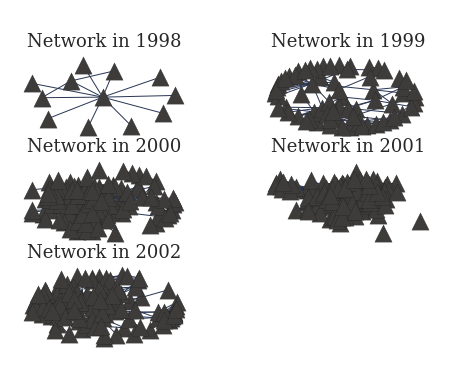
\includegraphics[height =0.7\textheight, width= 0.9\textwidth]{yearly_net.png}
    \caption{Node Link Diagram of yearly networks}
    \label{fig:Node Link Diagram for the yearly networks}
\end{figure}

\begin{figure}[H]
    \centering
    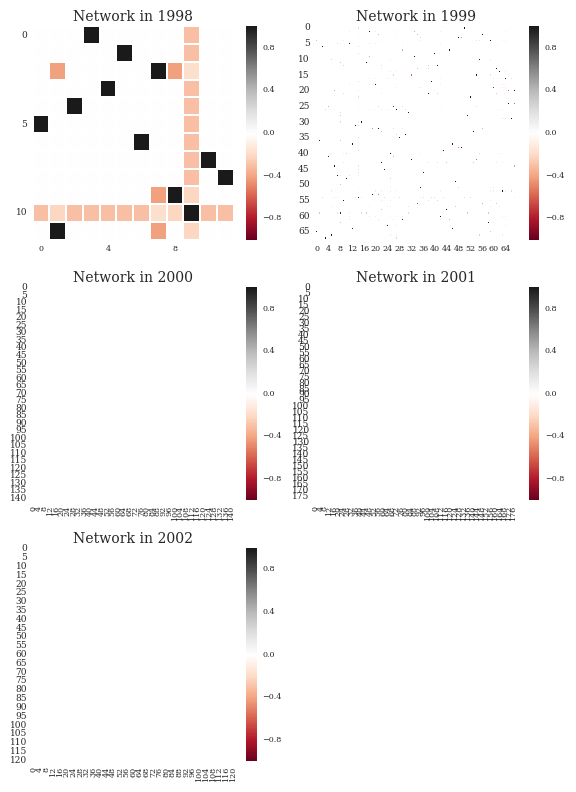
\includegraphics[height =0.9\textheight, width= 0.9\textwidth]{yearly_net_mat.png}
    \caption{Reordered Matrix Diagram of yearly networks}
    \label{fig:Reordered Matrix Diagram for the yearly networks}
\end{figure}

\begin{figure}[H]
    \centering
    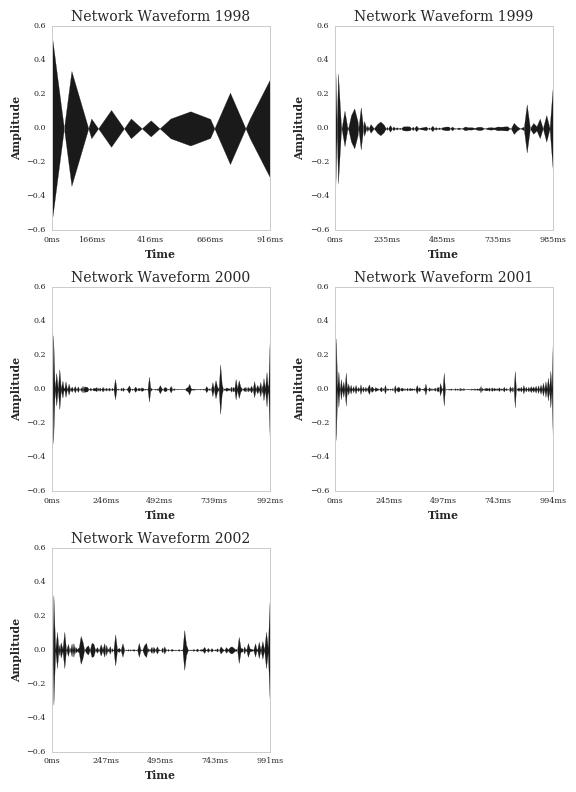
\includegraphics[height =0.9\textheight, width= 0.9\textwidth]{yearly_net_audio.png}
    \caption{Audio Waveform plot of yearly networks}
    \label{fig:Audio Waveform Plot for the yearly networks}
\end{figure}

\subsection{Monthly Network Visualisations}
\begin{figure}[H]
    \centering
    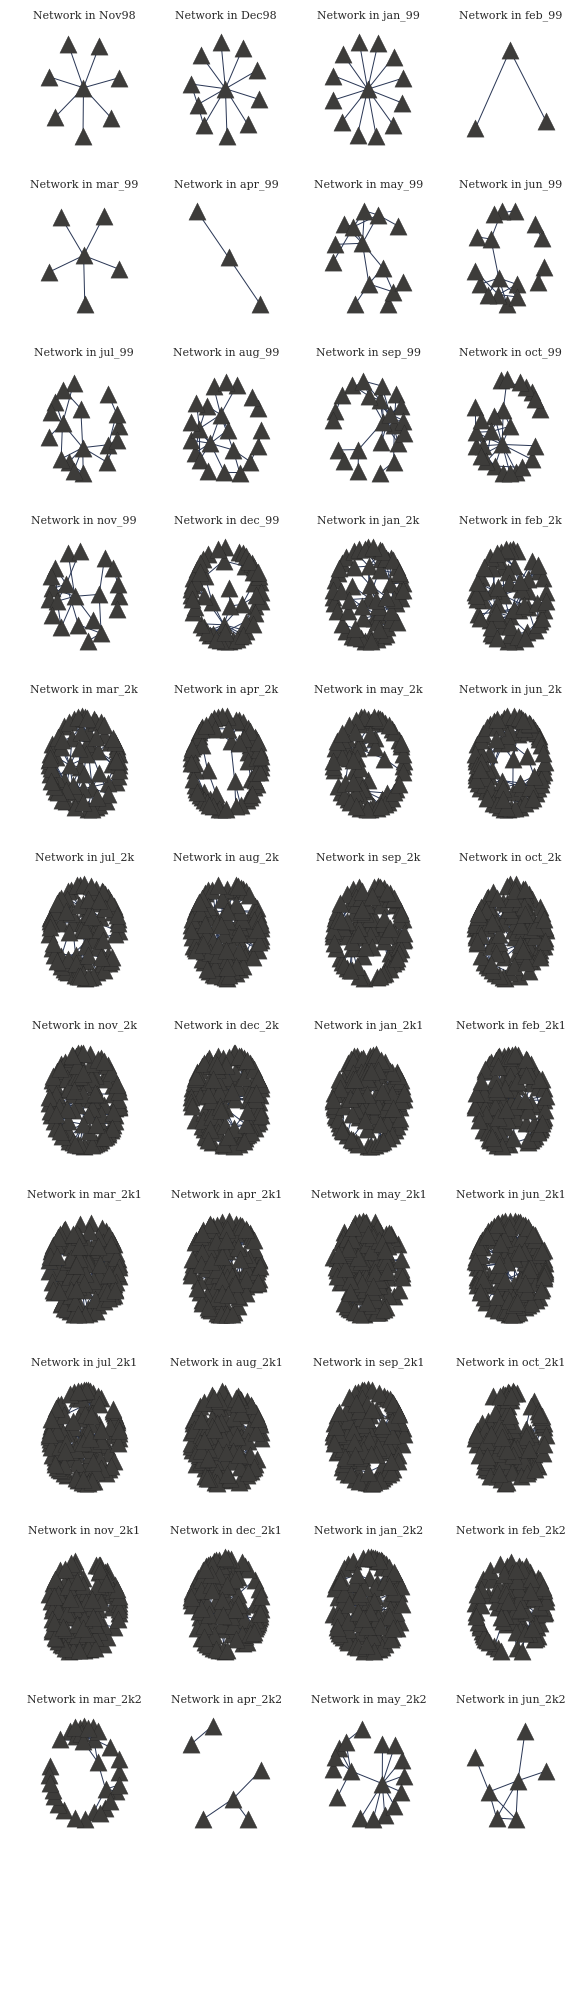
\includegraphics[height =0.9\textheight, width= 0.9\textwidth]{mth_net_nodelink.png}
    \caption{Node Link Diagram of monthly networks}
    \label{fig:node mth}
\end{figure}

\begin{figure}[H]
    \centering
    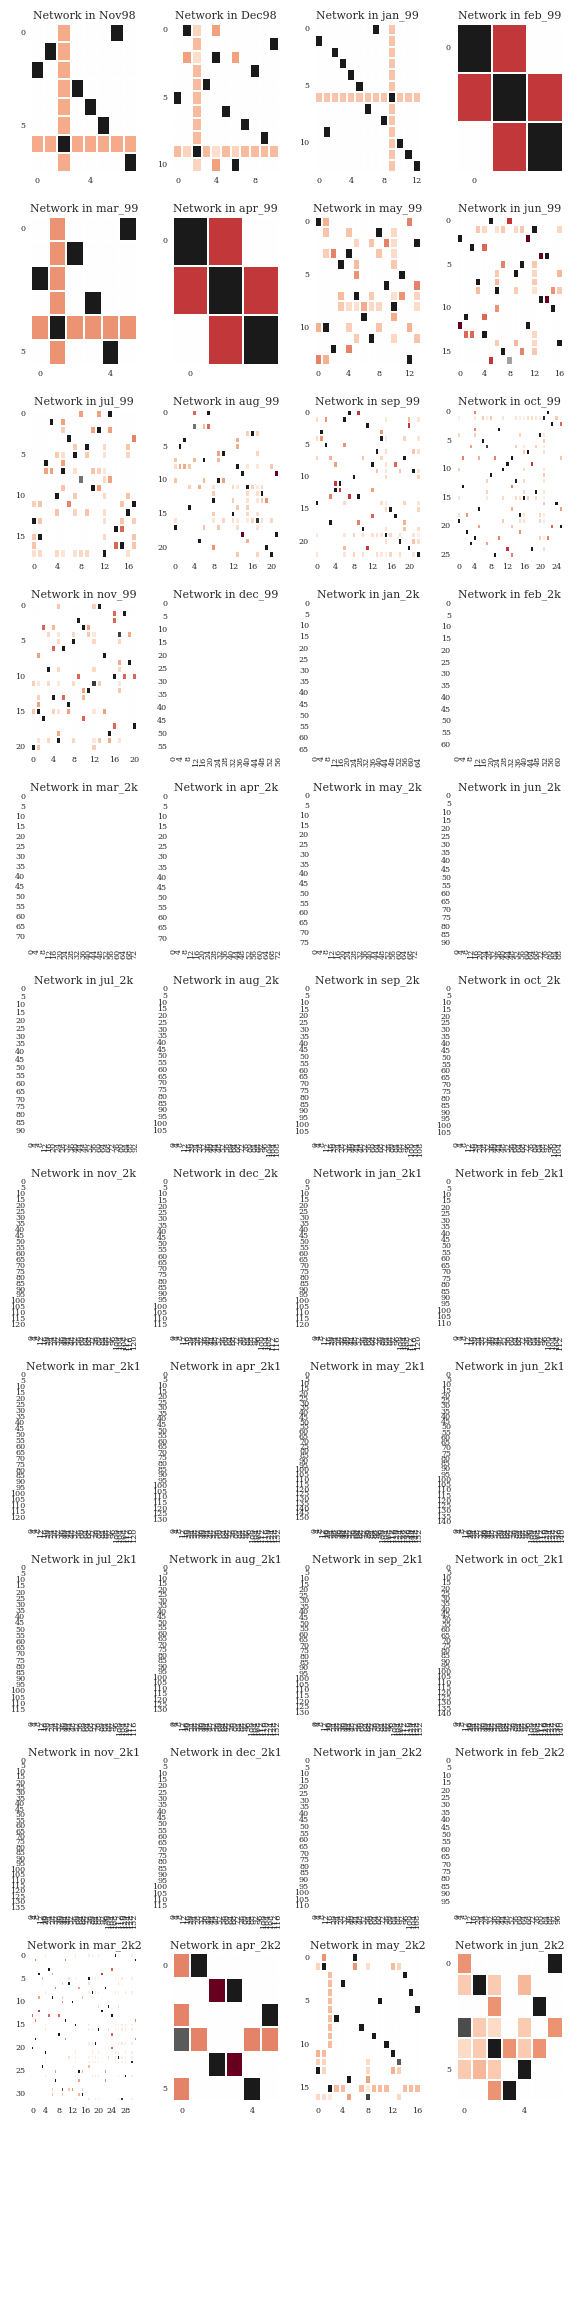
\includegraphics[height =0.9\textheight, width= 0.9\textwidth]{mth_net_mat.png}
    \caption{Reordered Matrix of monthly networks}
    \label{fig:Reordered Matrix Diagram for the monthly networks}
\end{figure}

\begin{figure}[H]
    \centering
    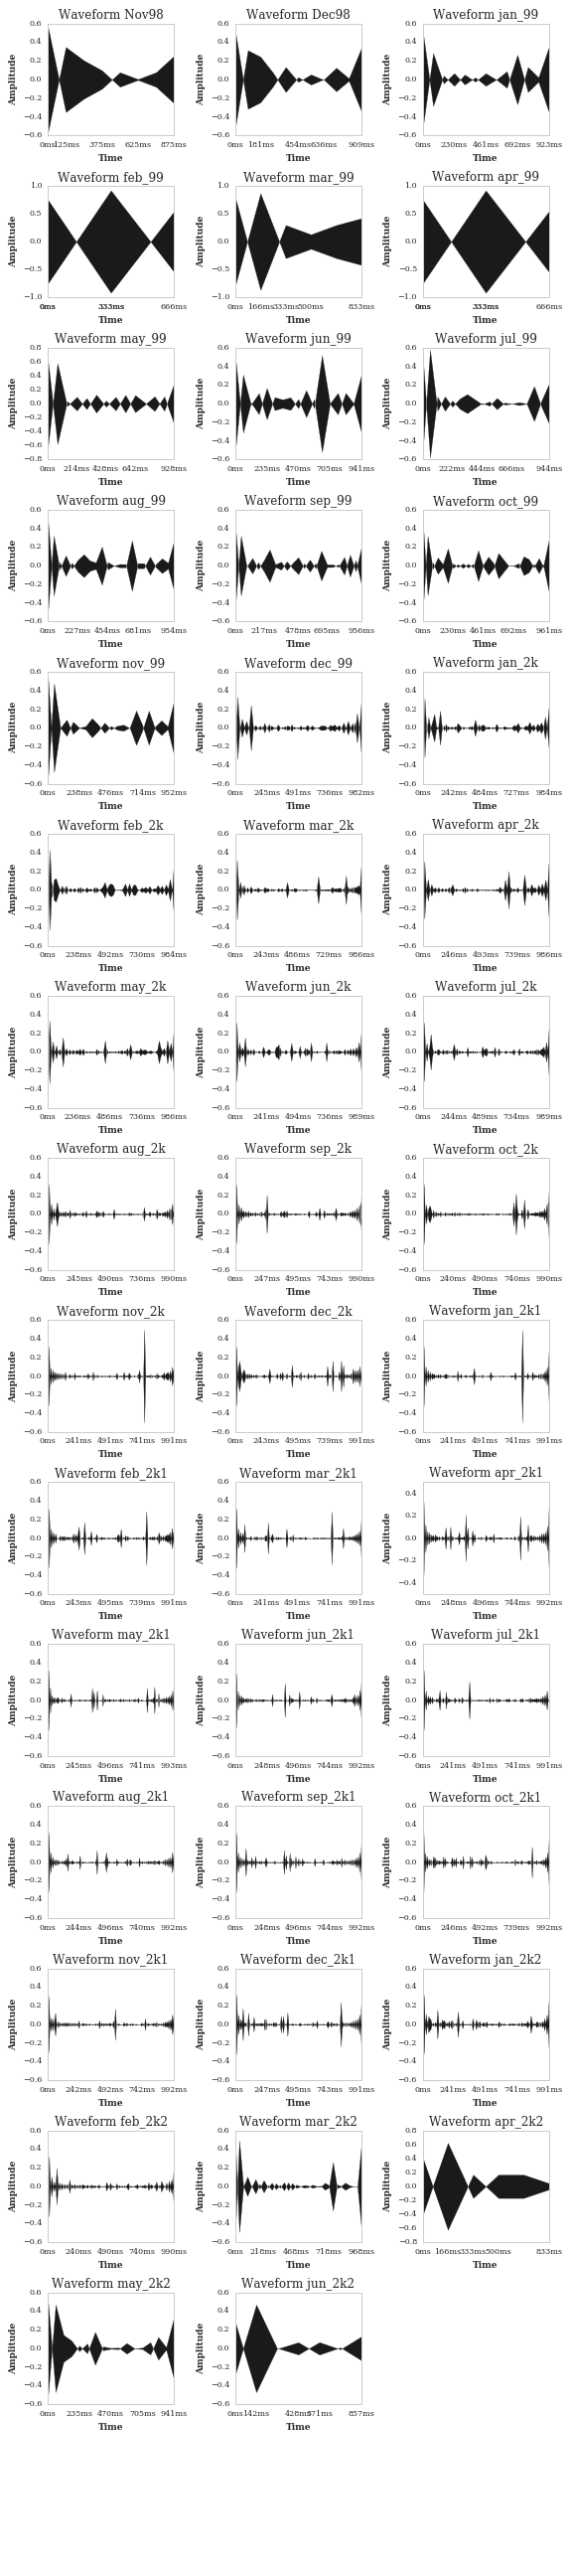
\includegraphics[height =0.9\textheight, width= 0.9\textwidth]{mth_net_audio.png}
    \caption{Audio Wavefrom  of monthly networks}
    \label{fig:Audio Waveform Plot for the monthly networks}
\end{figure}

\section{Exploratory Analysis: Centrality Measures} \label{explanal}

\subsection{Yearly Analysis}
\begin{figure}[H]
    \centering
    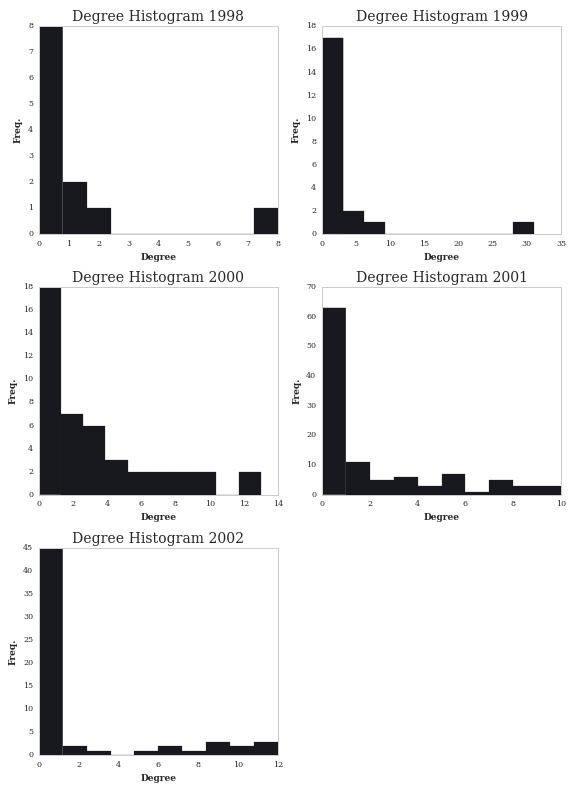
\includegraphics[height =0.9\textheight, width= 0.9\textwidth]{year_deghist.png}
    \caption{Yearly Degree Histogram}
    \label{fig:Yearly Degree Histogram}
\end{figure}

\begin{figure}[H]
    \centering
    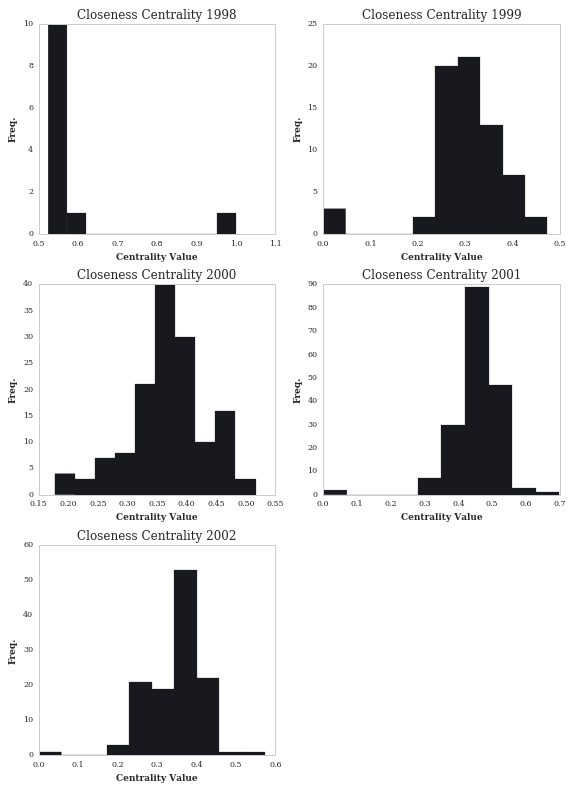
\includegraphics[height =0.9\textheight, width= 0.9\textwidth]{year_clohist.png}
    \caption{Yearly Closeness Centrality Histogram}
    \label{fig:Yearly Closeness Centrality Histogram}
\end{figure}

\begin{figure}[H]
    \centering
    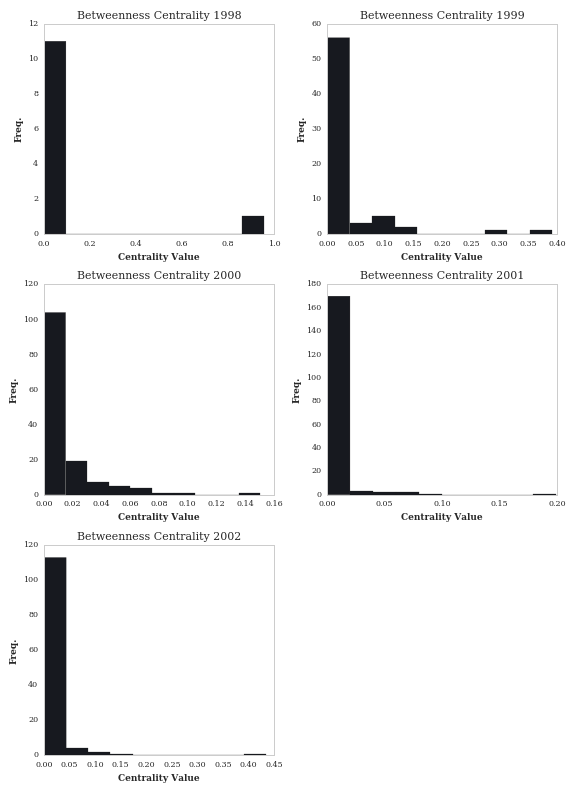
\includegraphics[height =0.9\textheight, width= 0.9\textwidth]{year_bethist.png}
    \caption{Yearly Betweenness Histogram}
    \label{fig:Yearly Betweenness Centrality Histogram}
\end{figure}

\begin{figure}[H]
    \centering
    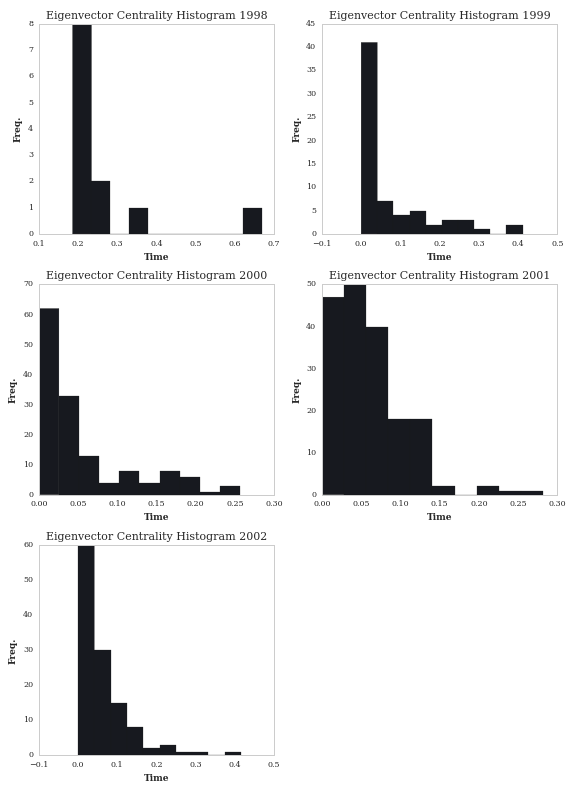
\includegraphics[height =0.9\textheight, width= 0.9\textwidth]{year_eighist.png}
    \caption{Yearly Eigenvector Centrality Histogram}
    \label{fig:Yearly Eigenvector Centrality Histogram}
\end{figure}

\begin{figure}[H]
    \centering
    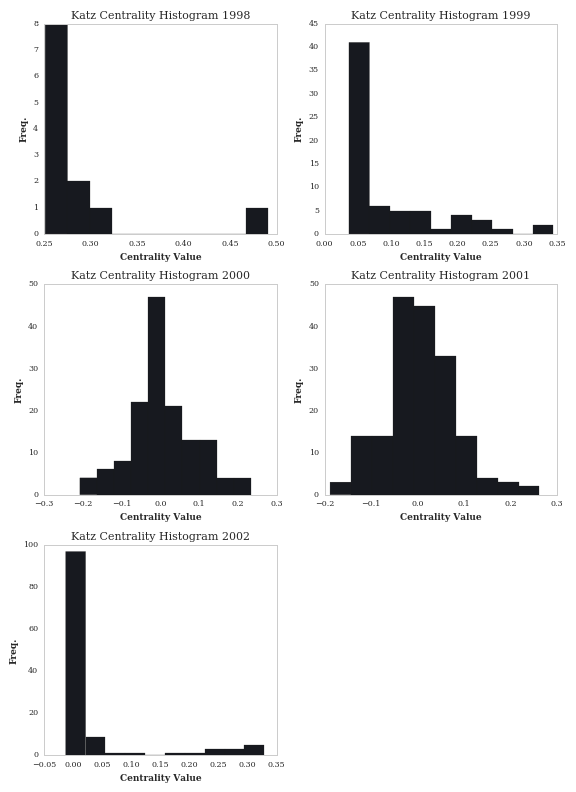
\includegraphics[height =0.9\textheight, width= 0.9\textwidth]{year_katzhist.png}
    \caption{Yearly Katz Centrality Histogram}
    \label{fig:Yearly Katz Centrality Histogram}
\end{figure}

\begin{figure}[H]
    \centering
    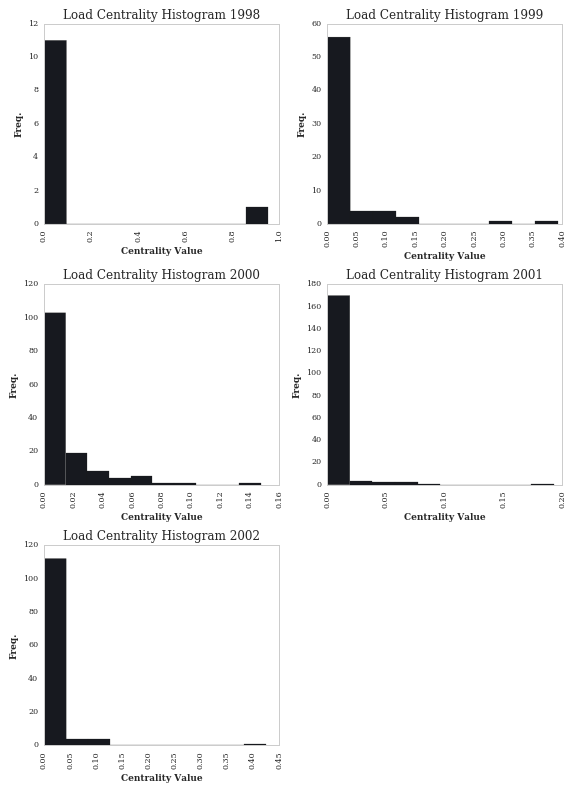
\includegraphics[height =0.9\textheight, width= 0.9\textwidth]{year_loadhist.png}
    \caption{Yearly Load Centrality Histogram}
    \label{fig:Yearly Load Centrality Histogram}
\end{figure}

\subsection{Monthly Analysis}
\begin{figure}[H]
    \centering
    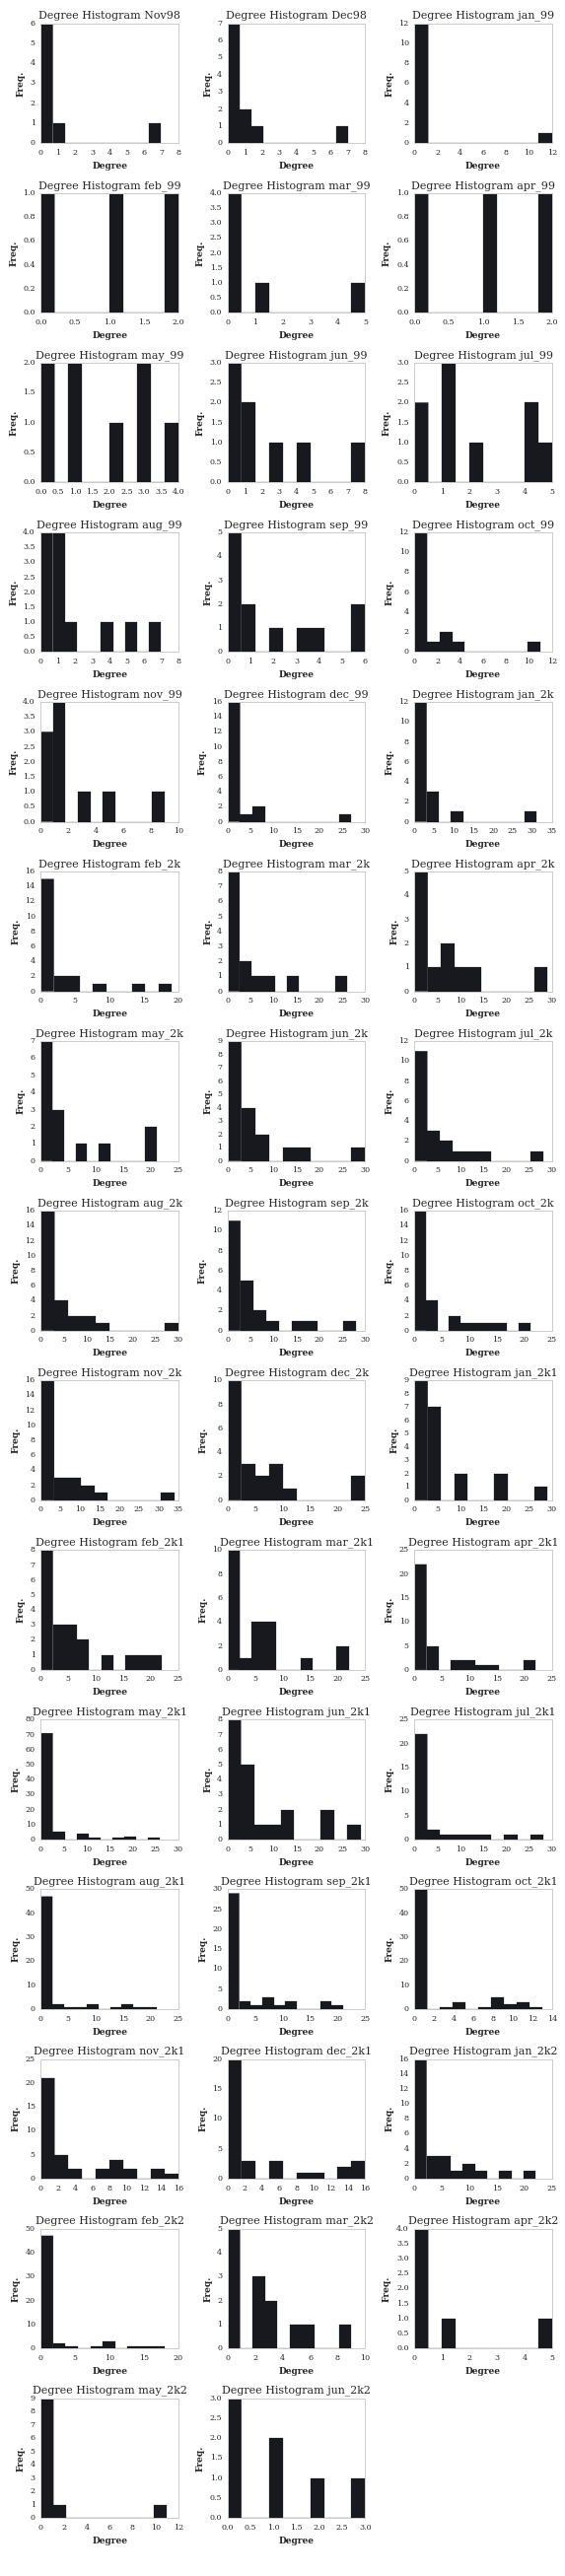
\includegraphics[height =0.9\textheight, width= 0.9\textwidth]{mth_deghist.png}
    \caption{Monthly Degree Histogram}
    \label{fig:Monthly Degree Histogram}
\end{figure}

\begin{figure}[H]
    \centering
    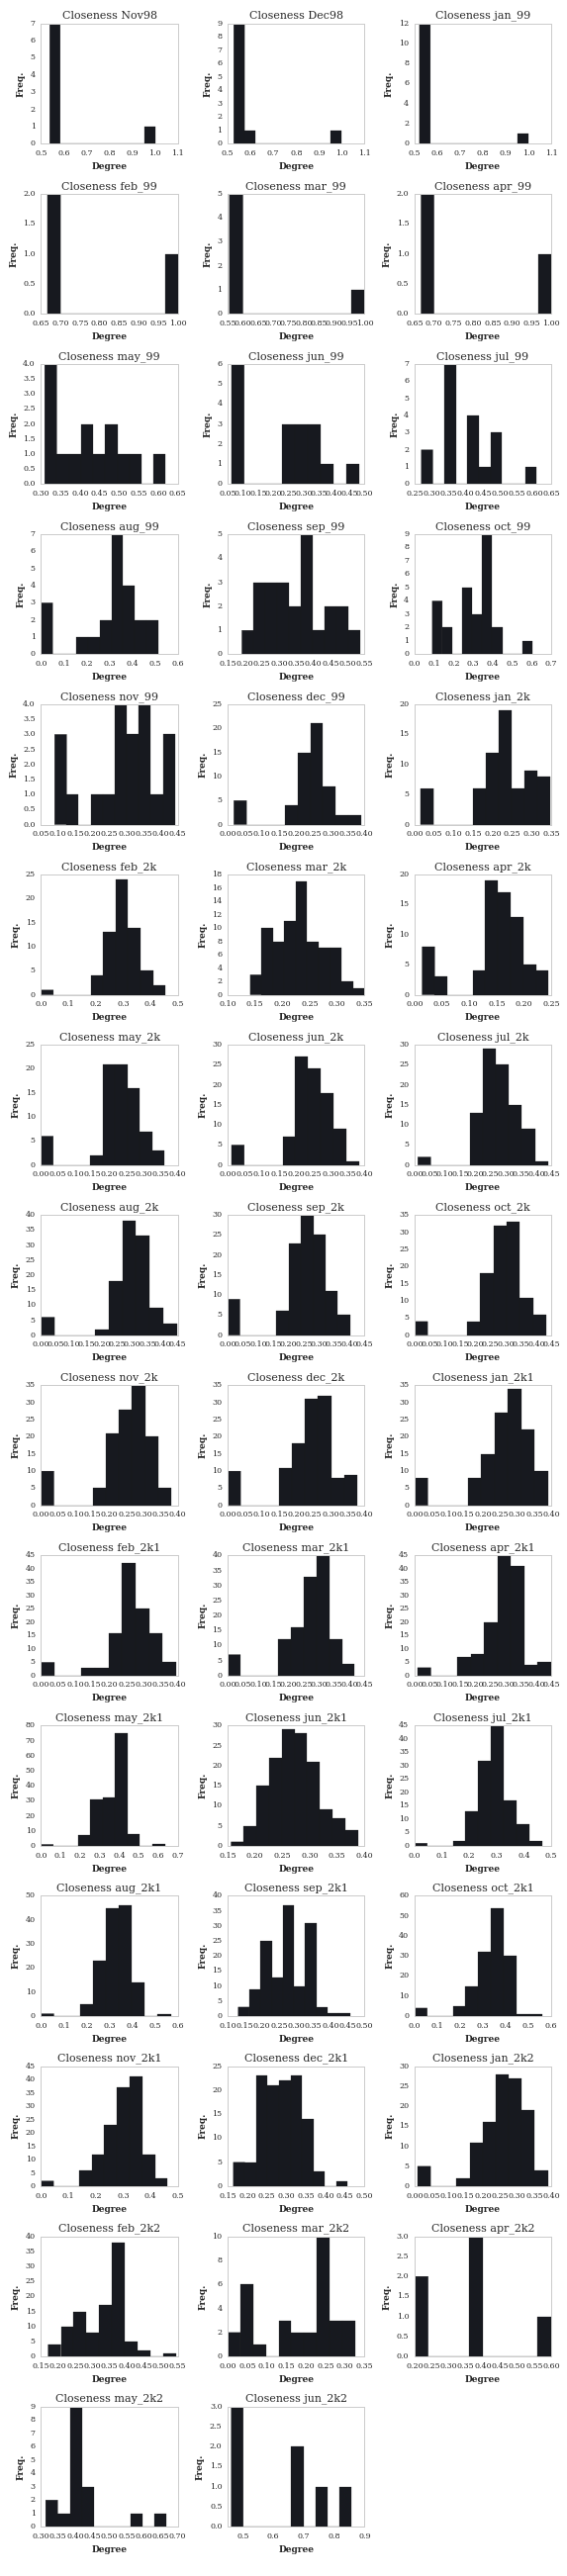
\includegraphics[height =0.9\textheight, width= 0.9\textwidth]{mth_clohist.png}
    \caption{Monthly Closeness Centrality Histogram}
    \label{fig:Monthly Closeness Centrality Histogram}
\end{figure}

\begin{figure}[H]
    \centering
    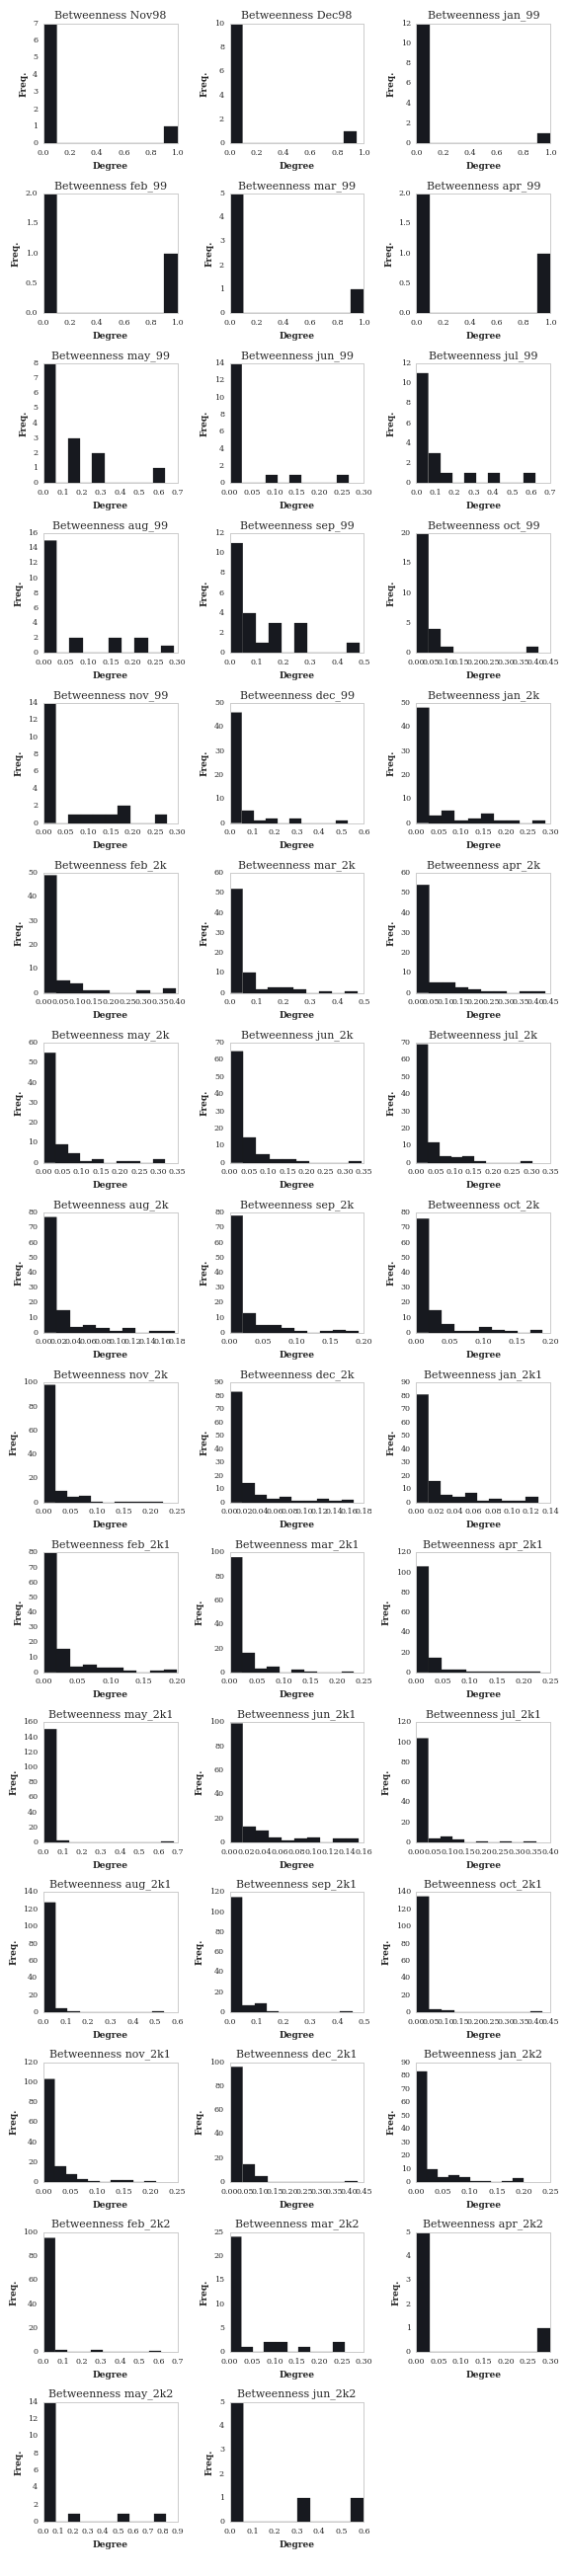
\includegraphics[height =0.9\textheight, width= 0.9\textwidth]{mth_bethist.png}
    \caption{Monthly Betweenness Histogram}
    \label{fig:Monthly Betweenness Centrality Histogram}
\end{figure}

\begin{figure}[H]
    \centering
    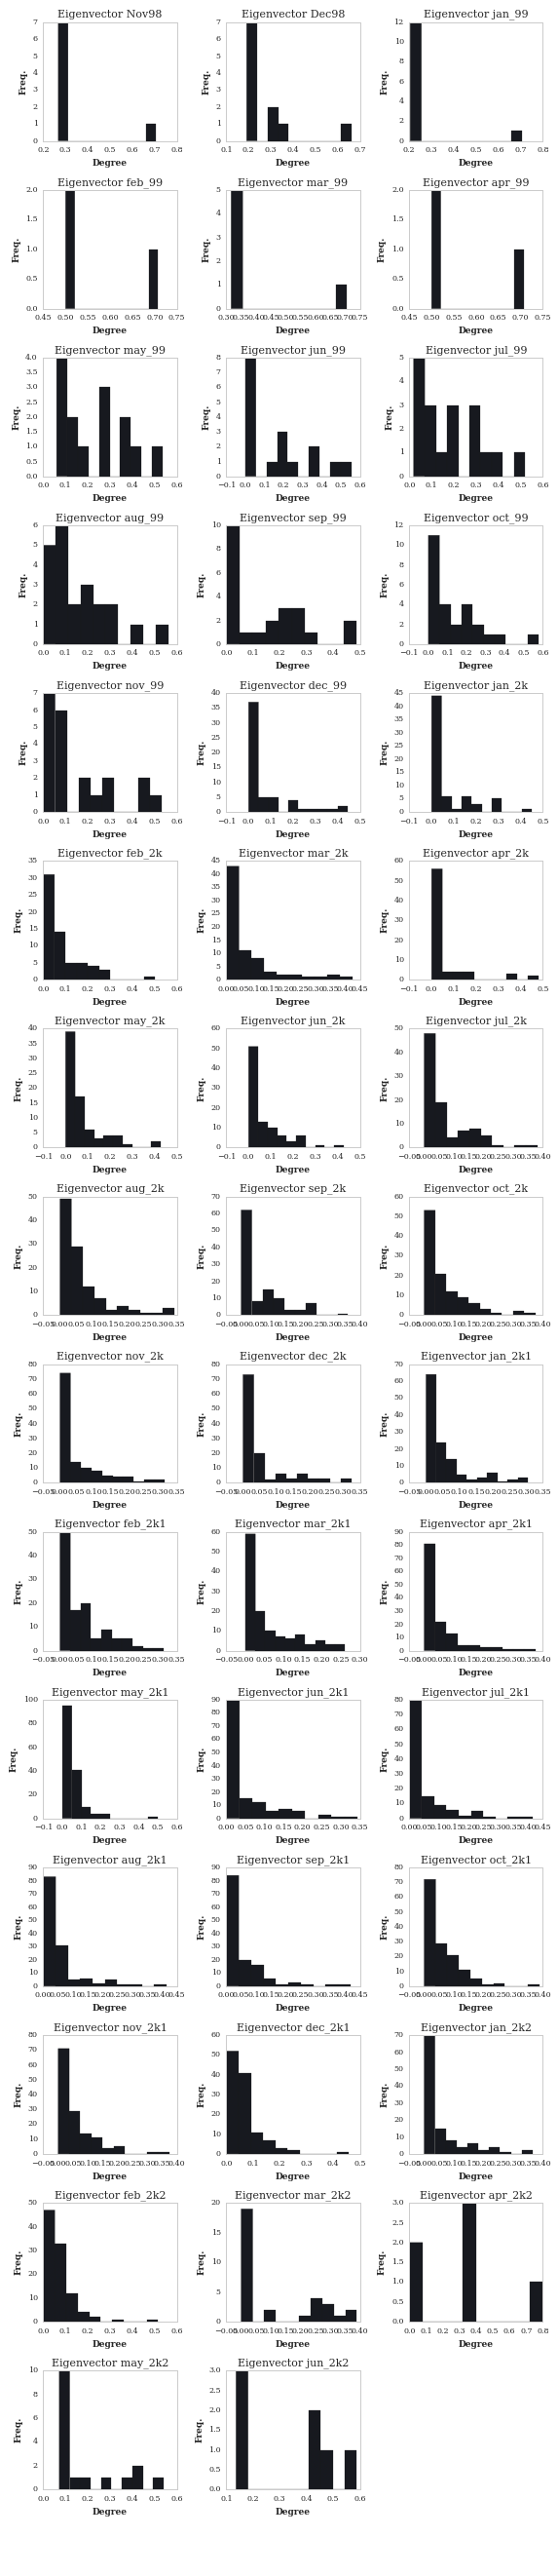
\includegraphics[height =0.9\textheight, width= 0.9\textwidth]{mth_eighist.png}
    \caption{Monthly Eigenvector Centrality Histogram}
    \label{fig:Monthly Eigenvector Centrality Histogram}
\end{figure}

\begin{figure}[H]
    \centering
    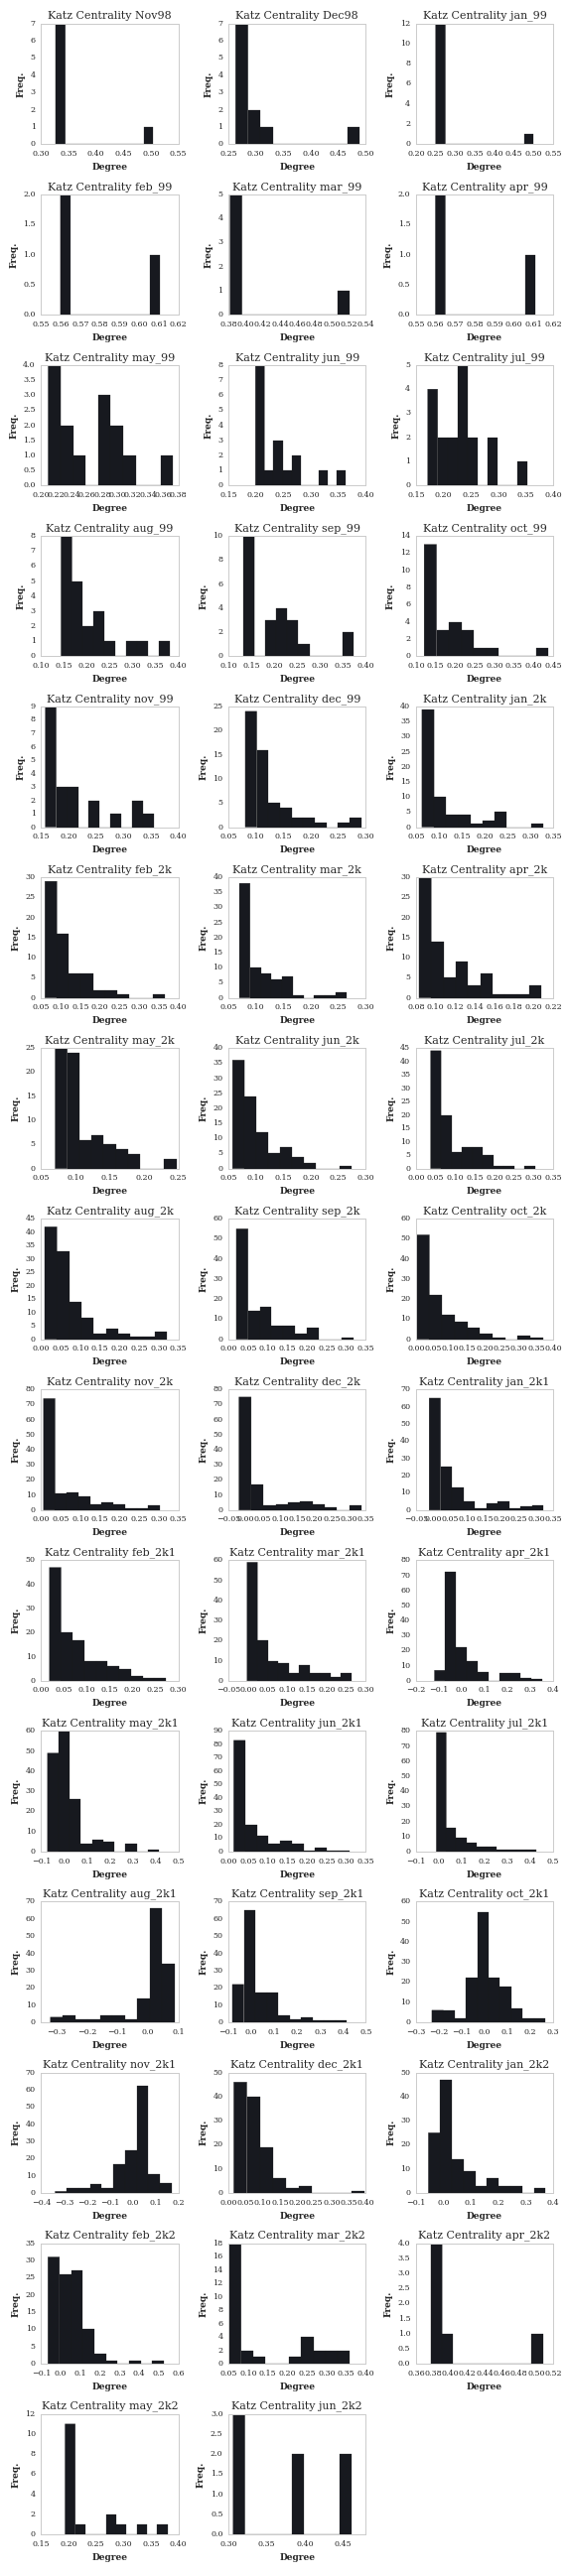
\includegraphics[height =0.9\textheight, width= 0.9\textwidth]{mth_katzhist.png}
    \caption{Monthly Katz Centrality Histogram}
    \label{fig:Monthly Katz Centrality Histogram}
\end{figure}

\begin{figure}[H]
    \centering
    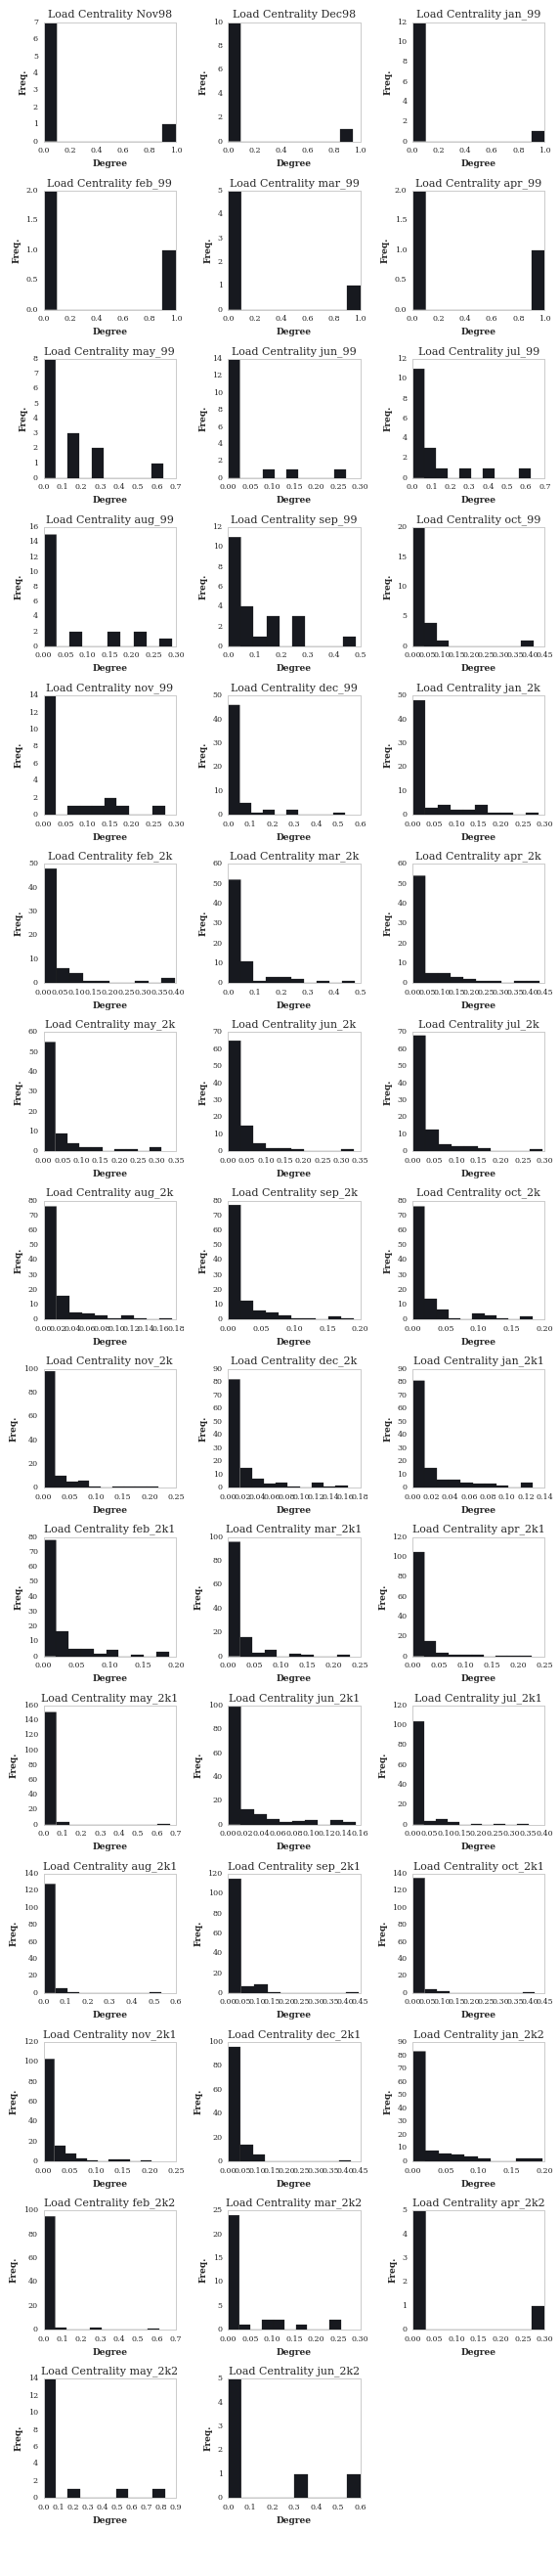
\includegraphics[height =0.9\textheight, width= 0.9\textwidth]{mth_loadhist.png}
    \caption{Monthly Load Centrality Histogram}
    \label{fig:Monthly Load Centrality Histogram}
\end{figure}

\section{Benchmark Measures}\label{bmark}

Here I plot the benchmark measures for the yearly and monthly networks to establish a signal in the graph time series. The measures proposed are judged firstly on their ability to model similar phenomenon and highlight additional interesting areas not obvious form these measures alone. \\

\begin{figure}[!htp]
    \centering
    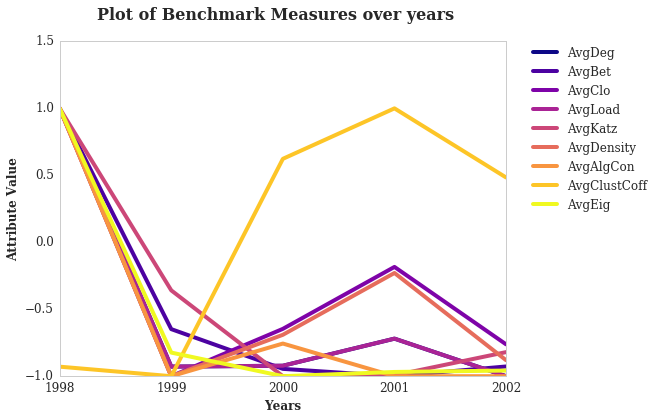
\includegraphics[height =0.3\textheight, width= 0.9\textwidth]{benchmark_yrs.png}
    \caption{Plot of Benchmark Measures over Years}
    \label{fig:bmark yrs}
\end{figure}

\begin{figure}[!htp]
    \centering
    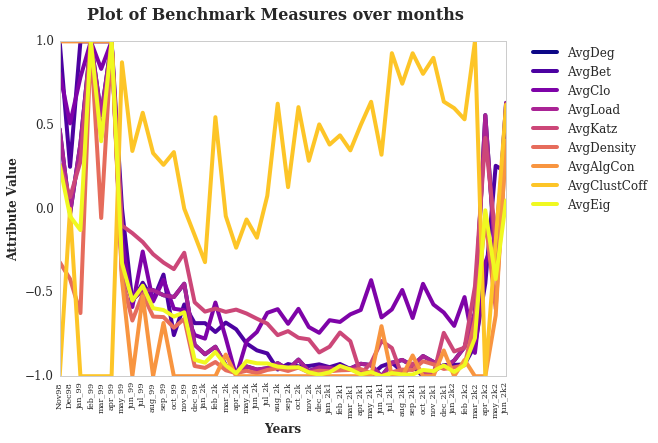
\includegraphics[height =0.3\textheight, width= 0.9\textwidth]{benchmark_mth.png}
    \caption{Plot of Benchmark Measures over Months}
    \label{fig:bmark mth}
\end{figure}

\clearpage{}
\section{Attribute Analysis}\label{attanal}

Here the novel measures proposed in this study are presented. First, I explore how the attributes vary when derived from different graph matrices.\\

\begin{figure}[!htp]
    \centering
    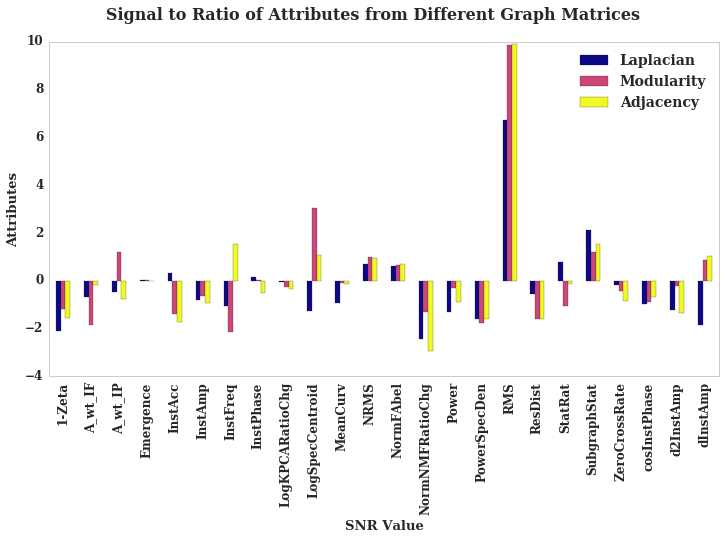
\includegraphics[height =0.4\textheight, width= 0.9\textwidth]{snr_allatt_3mat.png}
    \caption{Plot of Signal to Noise Ratio of Attributes calculated from 3 different Graph Matrices}
    \label{fig:snr}
\end{figure}

\begin{figure}[!htp]
    \centering
    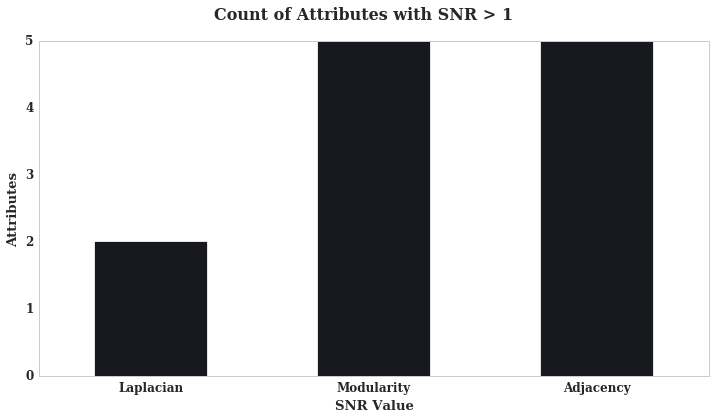
\includegraphics[height =0.3\textheight, width= 0.9\textwidth]{snrcount.png}
    \caption{Plot of Count of Number attributes with $SNR > 1$ from the different graph matrices}
    \label{fig:snr count}
\end{figure}

\begin{figure}[!htp]
    \centering
    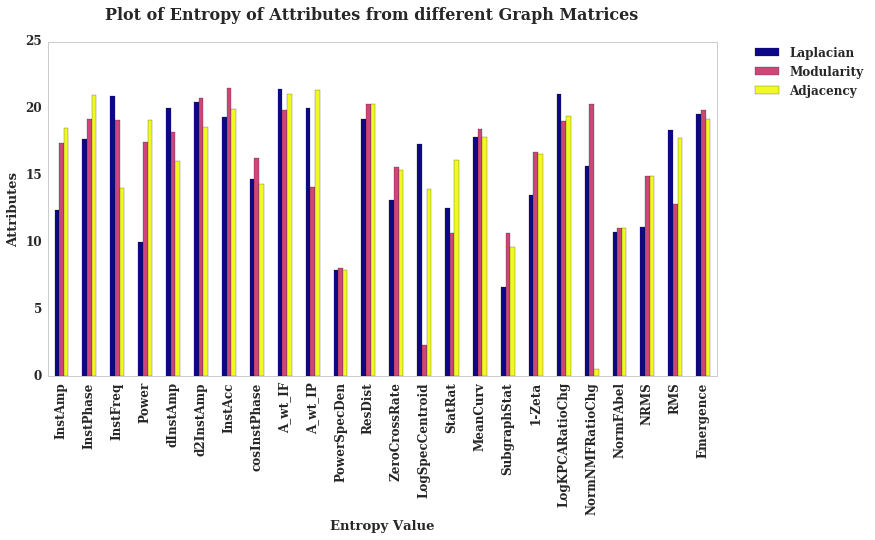
\includegraphics[height =0.5\textheight, width= 0.9\textwidth]{entropy.png}
    \caption{Plot of Entropy of attributes from the different graph matrices}
    \label{fig:entropy}
\end{figure}

\begin{figure}[!htp]
    \centering
    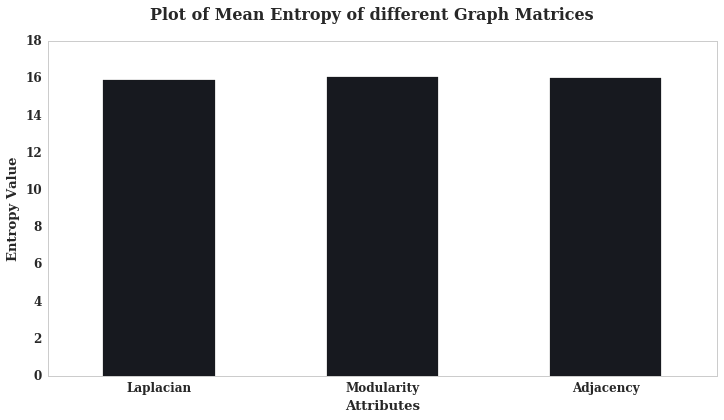
\includegraphics[height =0.4\textheight, width= 0.9\textwidth]{entropy_mean.png}
    \caption{Plot of Mean Entropy of different graph matrices}
    \label{fig:mean entropy}
\end{figure}


\begin{figure}[H]
    \centering
    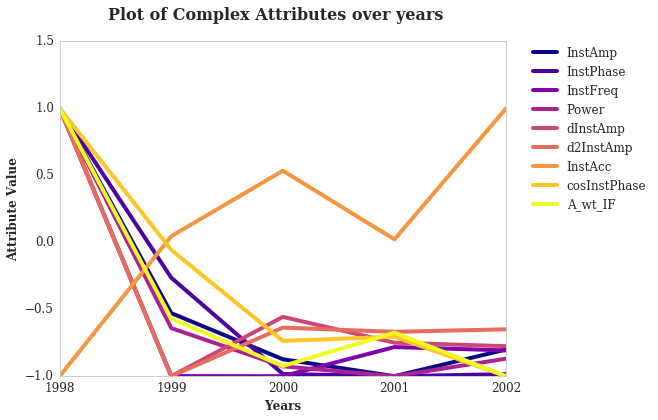
\includegraphics[height =0.4\textheight, width= 0.9\textwidth]{complex_yrs.png}
    \caption{Plot of Complex Attributes over Years}
    \label{fig:complex yrs}
\end{figure}

\begin{figure}[H]
    \centering
    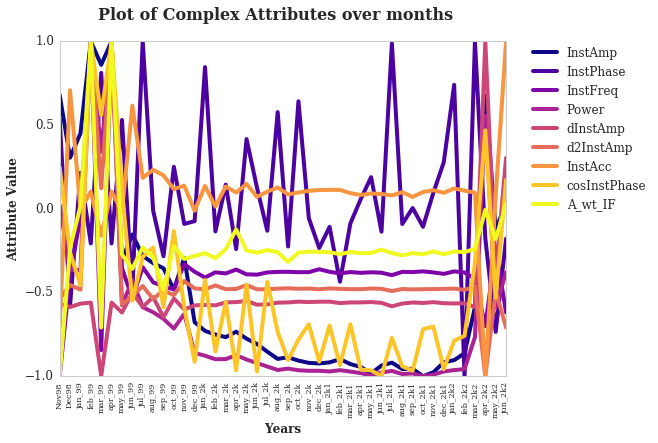
\includegraphics[height =0.4\textheight, width= 0.9\textwidth]{complex_mth.png}
    \caption{Plot of Complex Attributes over Months}
    \label{fig:compolex mth}
\end{figure}


\begin{figure}[H]
    \centering
    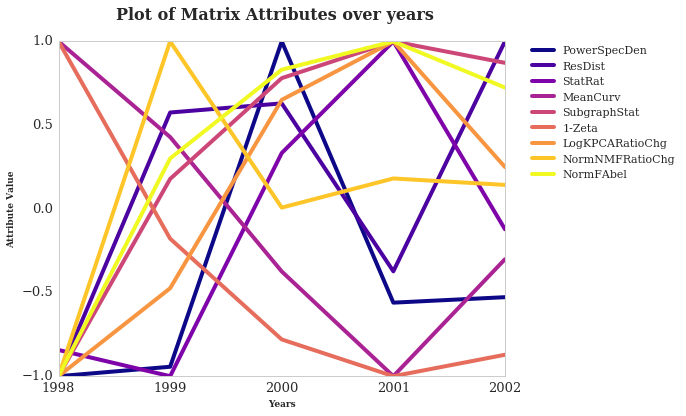
\includegraphics[height =0.4\textheight, width= 0.9\textwidth]{mat_yrs.png}
    \caption{Plot of Matrix Attributes over Months}
    \label{fig:mat yrs}
\end{figure}

\begin{figure}[H]
    \centering
    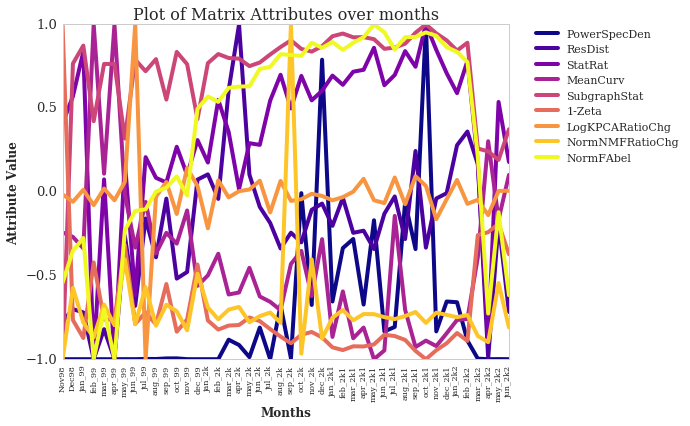
\includegraphics[height =0.4\textheight, width= 0.9\textwidth]{mat_mth.png}
    \caption{Plot of Matrix Attributes over Months}
    \label{fig:mat mth}
\end{figure}

\begin{figure}[H]
    \centering
    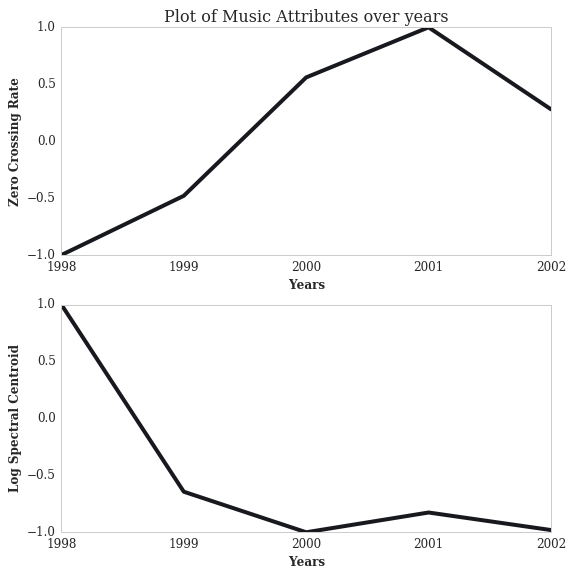
\includegraphics[height =0.4\textheight, width= 0.9\textwidth]{musicatt_yrs.png}
    \caption{Plot of Music Attributes over Years}
    \label{fig:music yrs}
\end{figure}

\begin{figure}[H]
    \centering
    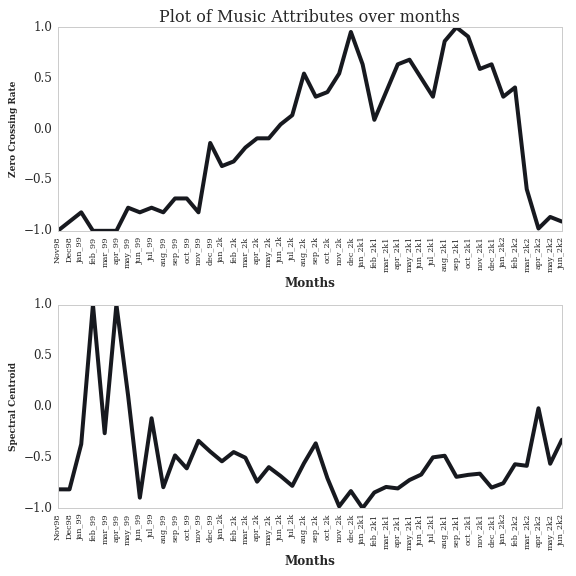
\includegraphics[height =0.4\textheight, width= 0.9\textwidth]{musicatt_mth.png}
    \caption{Plot of Music Attributes over Months}
    \label{fig:music mth}
\end{figure}

\clearpage{}
\subsection{Average Attributes}

\begin{figure}[H]
    \centering
    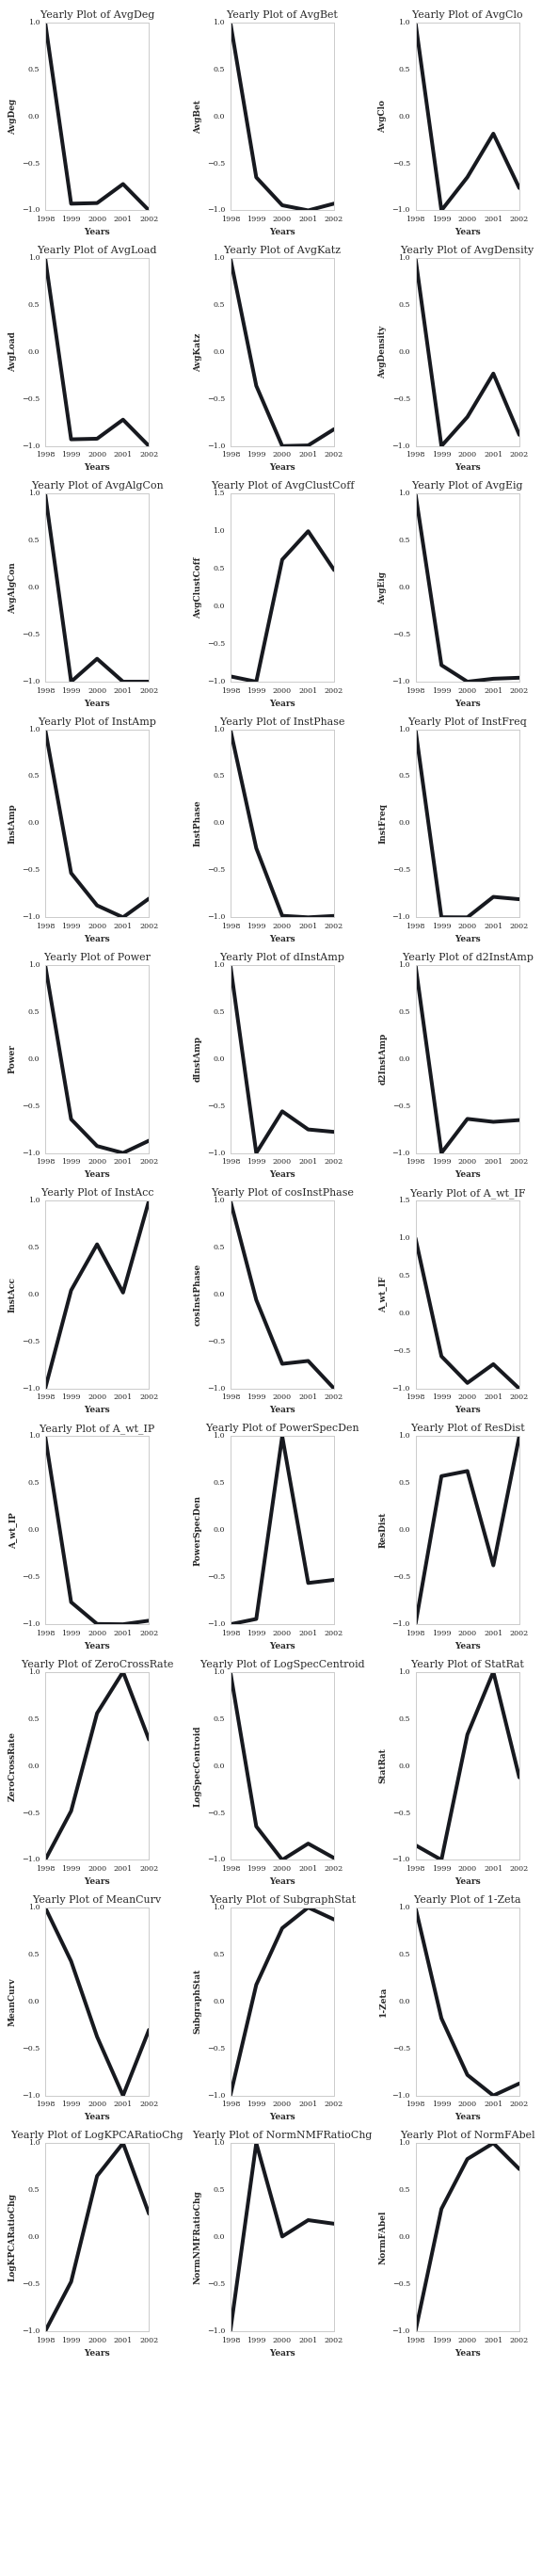
\includegraphics[height =0.9\textheight, width= 0.9\textwidth]{avg_allatt_yrs.png}
    \caption{Plot of Average Attributes over Years}
    \label{fig:avg all yrs}
\end{figure}

\begin{figure}[H]
    \centering
    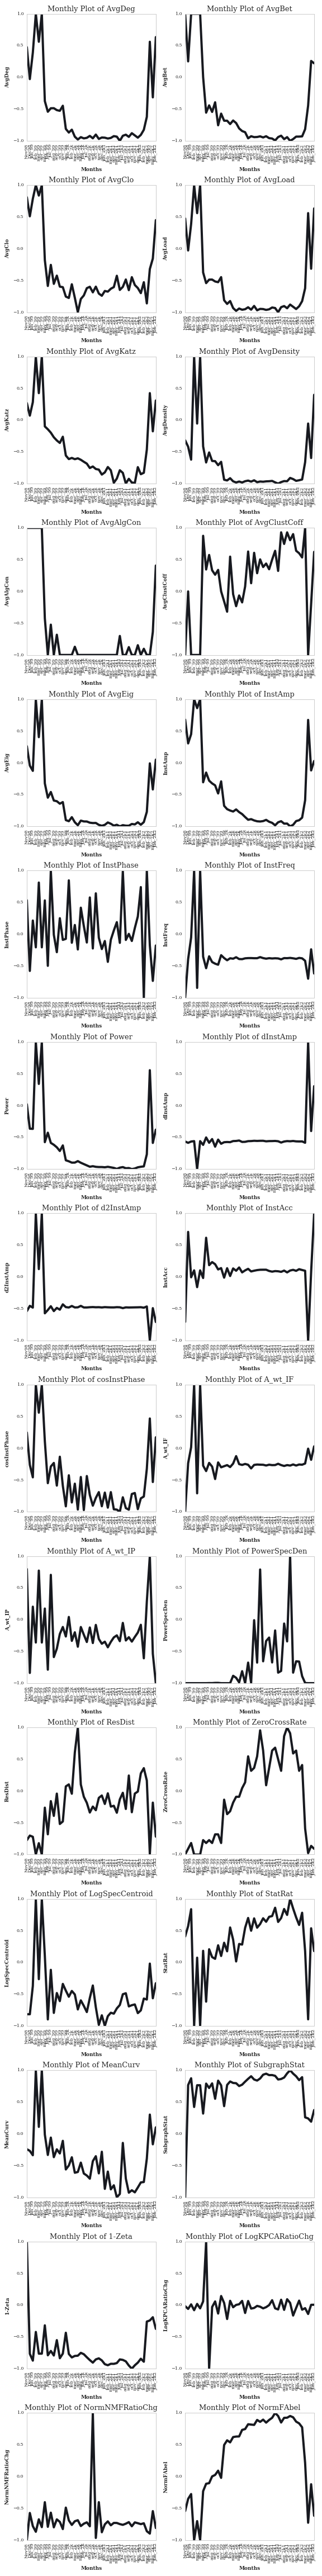
\includegraphics[height =0.9\textheight, width= 0.9\textwidth]{avg_allatt_mth.png}
    \caption{Plot of Average Attributes over Months}
    \label{fig:avg all mth}
\end{figure}

\clearpage{}
\section{Correlation Analysis}\label{corrfig}
 The correlation analysis is performed using the monthly level attributes because the yearly data has a very small sample size. Also the correlation measure used is the Pearson Correlation.\\

\begin{figure}[H]
    \centering
    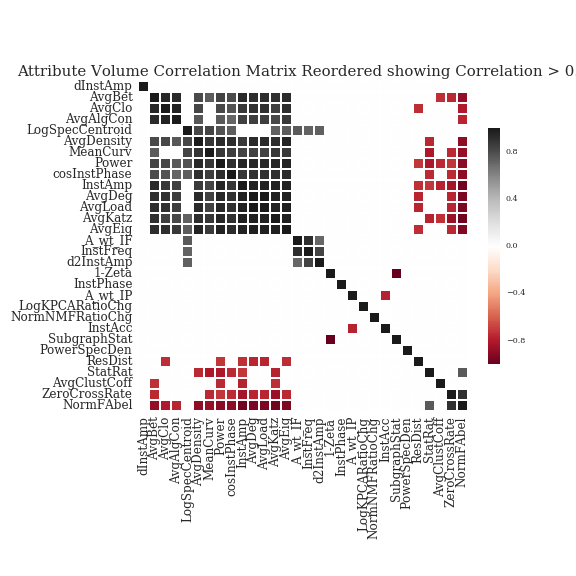
\includegraphics[height =0.8\textheight, width= 1\textwidth]{reordered_corrmat.png}
    \caption{Reordered Correlation Heatmap showing correlation $> 0.7$}
    \label{fig:Corrmat}
\end{figure}

\begin{figure}[H]
    \centering
    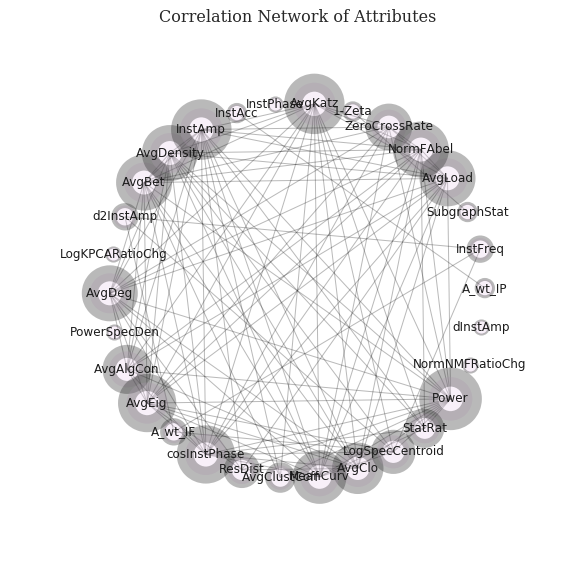
\includegraphics[height =0.4\textheight, width= 1\textwidth]{corrnet.png}
    \caption{Correlation Network of Attributes. The thickness of the borders of the nodes indicates high degree while low thickness of borders around the nodes indicate low degree.}
    \label{fig:CorrNet}
\end{figure}

\begin{figure}[H]
    \centering
    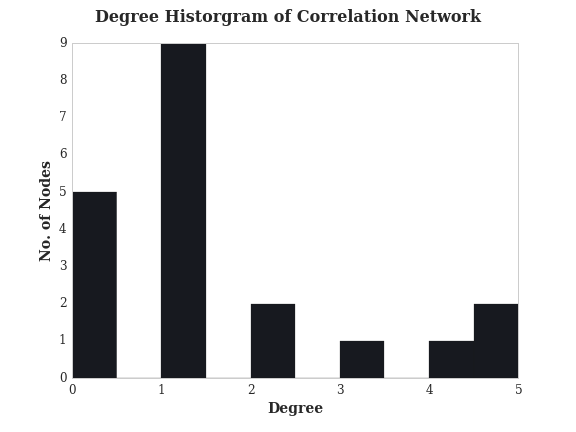
\includegraphics[height =0.4\textheight, width= 0.8\textwidth]{corrnet_deghist.png}
    \caption{Correlation Network Degree Histogram}
    \label{fig:CorrDegHist}
\end{figure}

\clearpage{}
\section{Feature Ranking with Regression Analysis}\label{regplots}

Here I used a Gradient Boosting Regressor with 10 boosting stages to predict the Average Degree of the network using the attribute volume. The test /train split is 50/50 to prevent over fitting. The Regressor produces a feature ranking of the variables and it is very useful to get a sense of the predictive potential of the measures. \\

\begin{figure}[!htp]
    \centering
    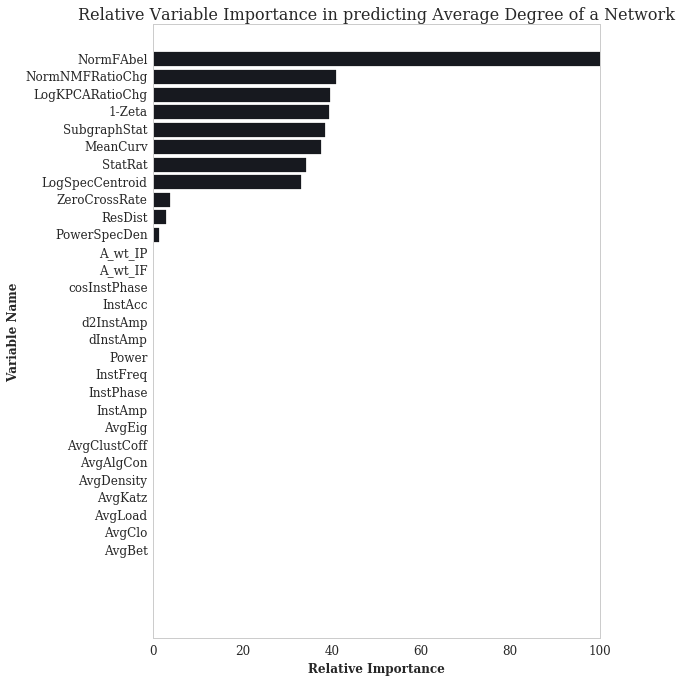
\includegraphics[height =0.5\textheight, width= 0.9\textwidth]{feature_ranking.png}
    \caption{Feature Ranking by Gradient Boosting Regressor for predicting Average Degree}
    \label{fig: featrank}
\end{figure}

\begin{figure}[!htp]
    \centering
    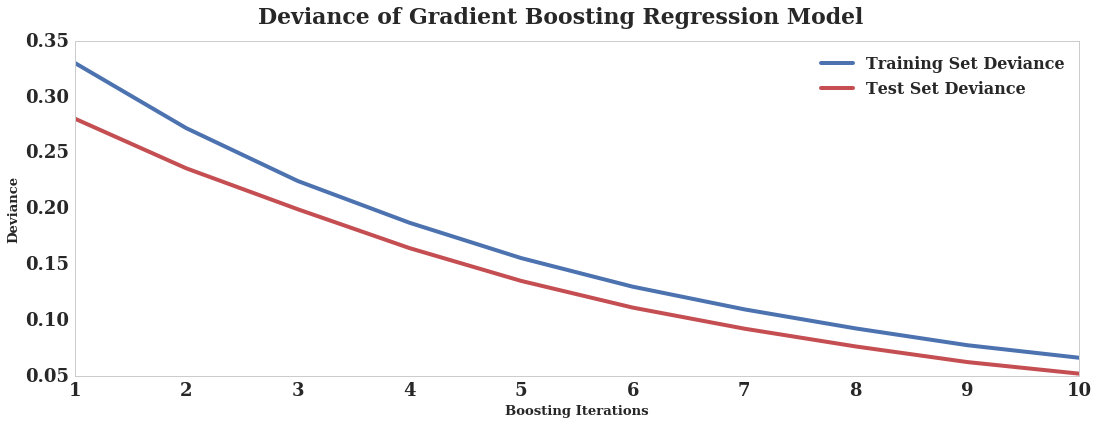
\includegraphics[height =0.2\textheight, width= 0.9\textwidth]{deviance.png}
    \caption{Regression Deviance Plot}
    \label{fig: regdev}
\end{figure}

\clearpage{}
\section{Aggregation Schemes}\label{aggplots}

\begin{figure}[!htp]
    \centering
    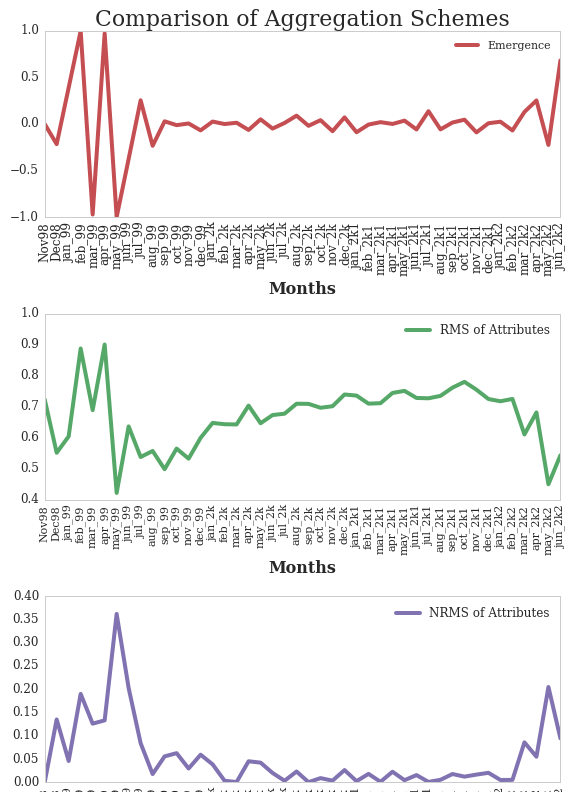
\includegraphics[height =0.9\textheight, width= 0.9\textwidth]{agg_comp.png}
    \caption{Comparison of different aggregation schemes.}
    \label{fig:aggcomp}
\end{figure}

\begin{figure}[!htp]
    \centering
    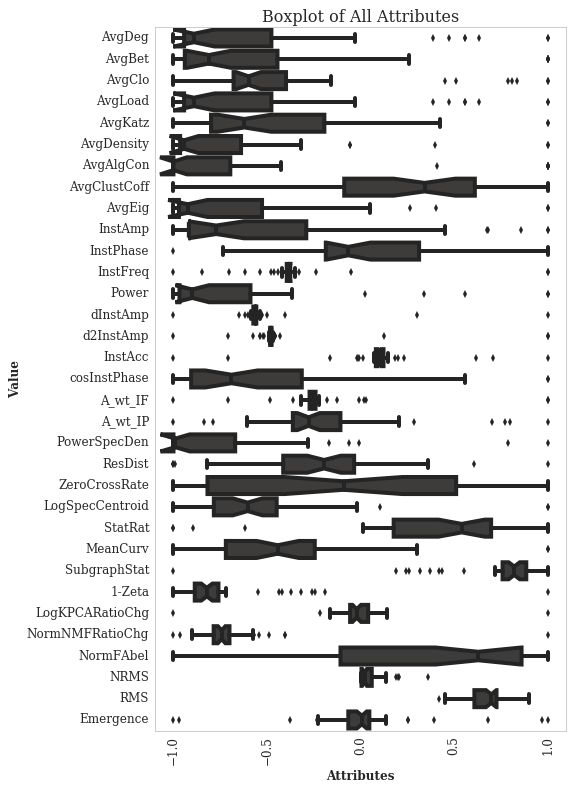
\includegraphics[height =0.9\textheight, width= 0.9\textwidth]{attvol_boxplot_all.png}
    \caption{Boxplot of All Attributes}
    \label{fig:boxplot}
\end{figure}

\clearpage{}
\section{Manifold Visualisation of Attribute Volume}\label{manifoldplots}
\begin{figure}[H]
    \centering
    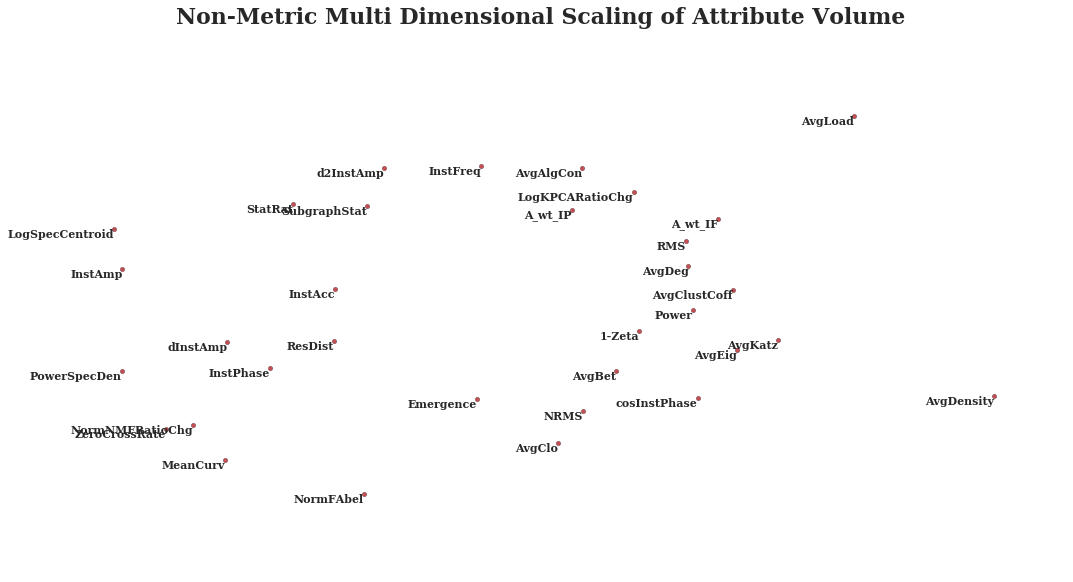
\includegraphics[height =0.4\textheight, width= 0.9\textwidth]{mds.png}
    \caption{Non-Metric Multidimensional Scaling of Attribute Volume}
    \label{fig:MDS}
\end{figure}

\begin{figure}[H]
    \centering
    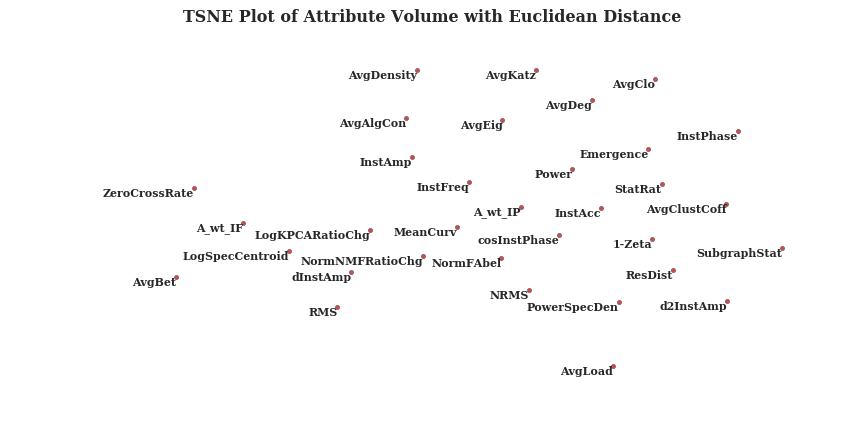
\includegraphics[height =0.4\textheight, width= 0.9\textwidth]{tsne_plot_euc.png}
    \caption{TSNE Plot of Attribute Volume with Euclidean Distance}
    \label{fig:TSNE Euclid}
\end{figure}

\begin{figure}[H]
    \centering
    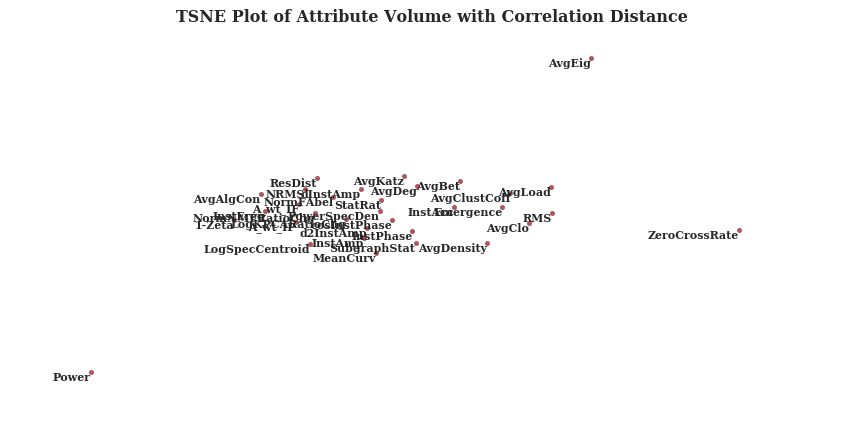
\includegraphics[height =0.4\textheight, width= 0.9\textwidth]{tsne_plot_corr.png}
    \caption{TSNE Plot of Attribute Volume with Correlation Distance}
    \label{fig:TSNE}
\end{figure}

\begin{figure}[H]
    \centering
    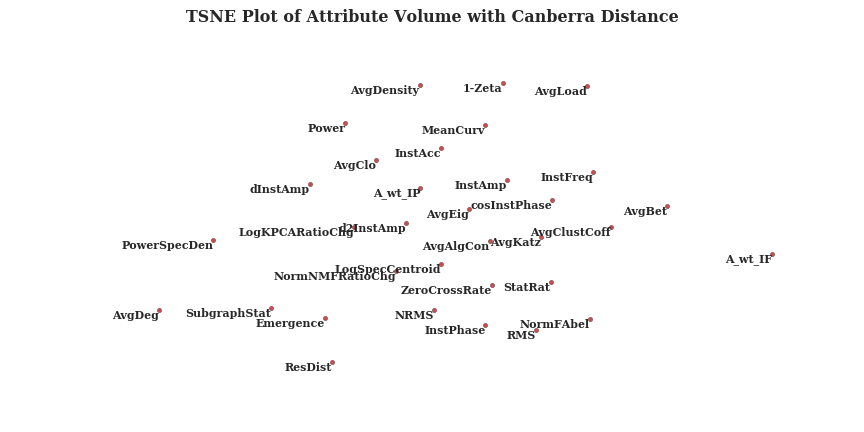
\includegraphics[height =0.4\textheight, width= 0.9\textwidth]{tsne_plot.png}
    \caption{TSNE Plot of Attribute Volume with Canberra Distance}
    \label{fig:TSNE}
\end{figure}

\clearpage{}
\section{FK and Radon Plots}\label{seisplots}

\begin{figure}[!htp]
    \centering
    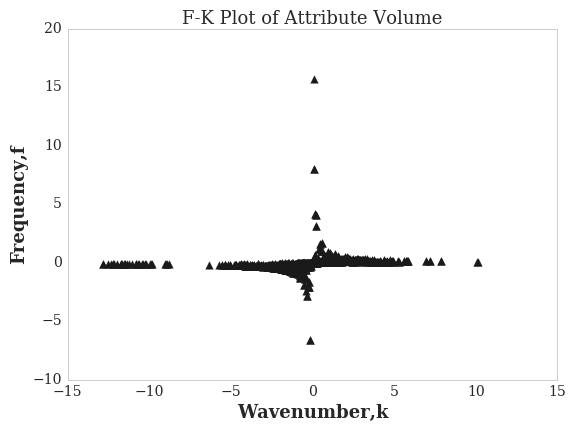
\includegraphics[height =0.4\textheight, width= 0.9\textwidth]{fkplot.png}
    \caption{Frequency Wavenumber (FK) Plot of Attribute Volume}
    \label{fig: fkplot}
\end{figure}

\begin{figure}[!htp]
    \centering
    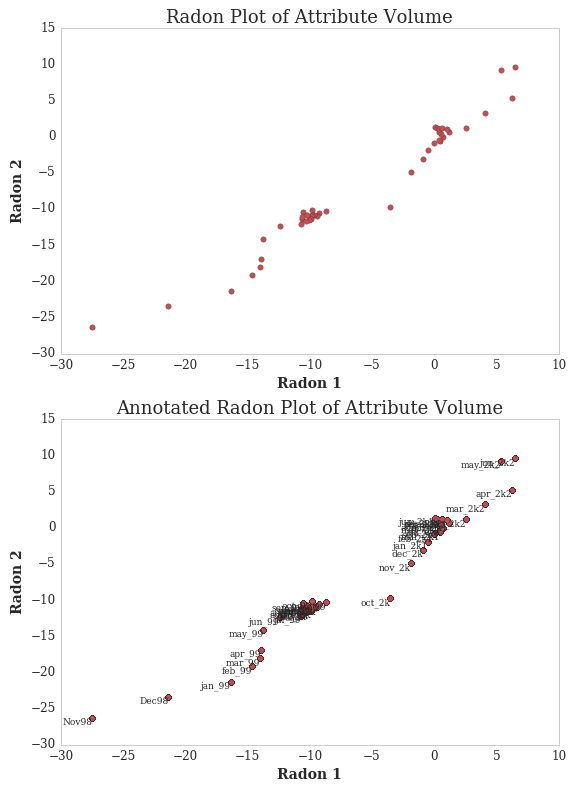
\includegraphics[height =0.4\textheight, width= 0.9\textwidth]{radonplot.png}
    \caption{(top) Radon Plot of Attribute Volume, (bottom) Annotated Radon Plot}
    \label{fig: radonplot}
\end{figure}


\begin{figure}[!htp]
    \centering
    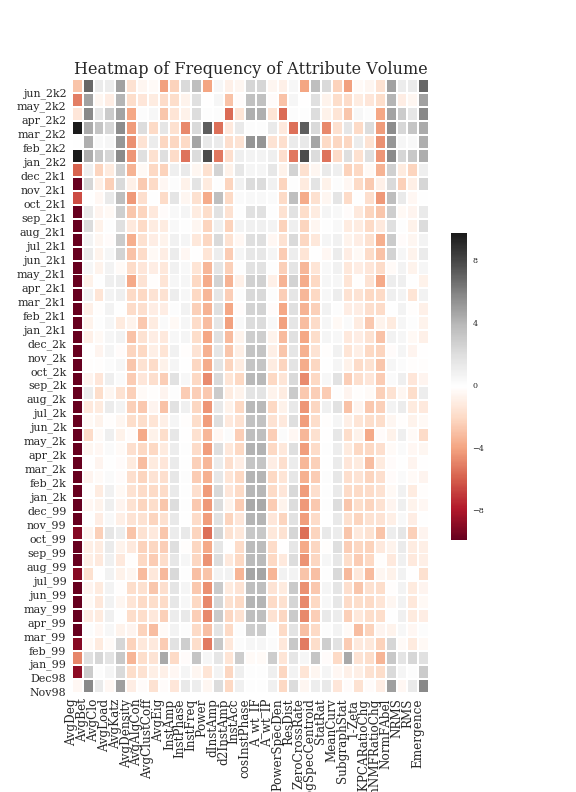
\includegraphics[height =0.4\textheight, width= 0.9\textwidth]{freq_heat.png}
    \caption{Heatmap of Frequency of Attribute Volume. This is the F component derived from the FK Plot}
    \label{fig:Frequency Heatmap}
\end{figure}

\begin{figure}[!htp]
    \centering
    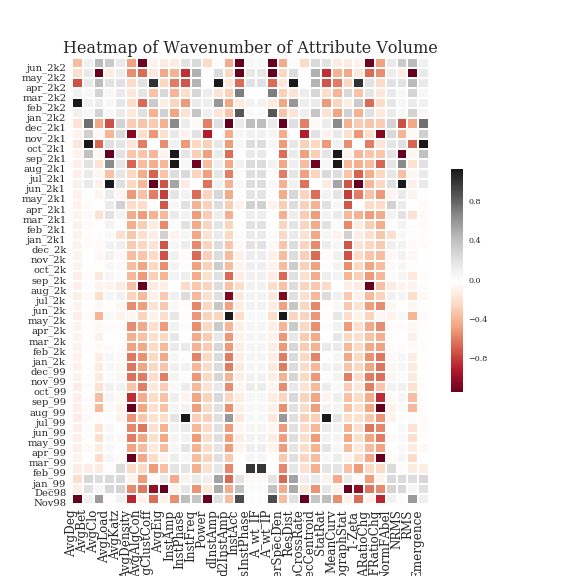
\includegraphics[height =0.4\textheight, width= 0.9\textwidth]{wavnum_heat.png}
    \caption{Heatmap of Wavenumber of Attribute Volume. This is the K component derived from the FK Plot}
    \label{fig:Wavenumber Heatmap}
\end{figure}

\begin{figure}[!htp]
    \centering
    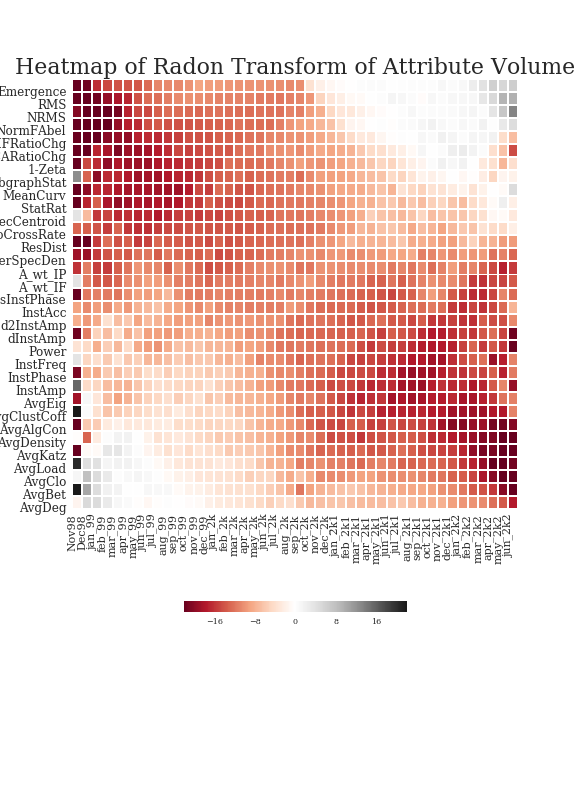
\includegraphics[height =0.7\textheight, width= 0.9\textwidth]{radon_heat.png}
    \caption{Heatmap of Radon Transform of Attribute Volume}
    \label{fig: Radon Heatmap}
\end{figure}

\begin{sidewaysfigure}
    \includegraphics[width=\textwidth]{logpanel.PNG}
    \caption{Log Panel of selected attributes. Benchmark attributes are shown in red. Seismic Attributes shown in blue. Music Attributes shown in yellow. Matrix Attributes shown in green and NRMS aggregation measure in black.}
    \label{fig: logpanel}
\end{sidewaysfigure}

\clearpage{}
\section{Node Level Trends}\label{nodeplots}

In this section I find common nodes across the 5 years and compare their centrality trends over time. The yearly trends for this part of the analysis is conducted as this is more plausible. The reason being that although these nodes are common across the years they do not have activity regularly across all months. Therefore it is deemed more informative to get an overview of their yearly centrality measure changes.\\

\begin{figure}[!htp]
    \centering
    \includegraphics[height =0.3\textheight, width= 0.7\textwidth]{node_deg.png}
    \caption{Plot of Common Node Degree over years}
    \label{fig: Plot of Common Node Degree Centrality over years}
\end{figure}

\begin{figure}[!htp]
    \centering
    \includegraphics[height =0.3\textheight, width= 0.7\textwidth]{node_bet.png}
    \caption{Plot of Common Node Betweenness Centrality over years}
    \label{fig: Plot of Common Node Betweenness Centrality over years}
\end{figure}

\begin{figure}[!htp]
    \centering
    \includegraphics[height =0.4\textheight, width= 0.7\textwidth]{node_clo.png}
    \caption{Plot of Common Node Closeness Centrality over years}
    \label{fig: Plot of Common Node Closeness Centrality over years}
\end{figure}

\begin{figure}[!htp]
    \centering
    \includegraphics[height =0.4\textheight, width= 0.7\textwidth]{node_eig.png}
    \caption{Plot of Common Node Eigenvector Centrality over years}
    \label{fig: Plot of Common Node Eigenvector Centrality over years}
\end{figure}

\begin{figure}[!htp]
    \centering
    \includegraphics[height =0.4\textheight, width= 0.7\textwidth]{node_katz.png}
    \caption{Plot of Common Node Katz Centrality over years}
    \label{fig: Plot of Common Node Katz Centrality over years}
\end{figure}

\begin{figure}[!htp]
    \centering
    \includegraphics[height =0.4\textheight, width= 0.7\textwidth]{node_load.png}
    \caption{Plot of Common Node Load Centrality over years}
    \label{fig: Plot of Common Node Load Centrality over years}
\end{figure}

\clearpage{}
\section{Discussion of Results}

In this section we have shown the results of the methods discussed extensively in Chapter 3. To begin with we started with some familiar visualisations such as node link and matrix diagrams of the networks at the yearly and monthly intervals. These are denoted in \Cref{fig:Node Link Diagram for the yearly networks,fig:node mth,fig:Reordered Matrix Diagram for the yearly networks,fig:Reordered Matrix Diagram for the monthly networks}.\\

From the yearly plots we see that the network is most sparse in 1998 and gradually gets more dense throughout the time period and then shrinks again in 2002. This is reflected in the waveform plots in  \Cref{fig:Audio Waveform Plot for the yearly networks,fig:Audio Waveform Plot for the monthly networks}. Here we see that the signal for 1999 is very blocky indicating probably that not many nodes are present in the network hence the amplitude envelope is smooth and blocky. But in the cases where the networks are dense we see that the signal is spiky indicating the greater number of nodes who have an associated amplitude and some have higher amplitude than others. These nodes are probably the more central players in the network. This is reflected at the monthly level as well as the first few months of the graph time series the networks are comparatively sparse compared to the middle. The network starts to thin out in the last few months of the time range. \\

The exploratory centrality histograms at the year and monthly level are what is observed in networks more generally. This is that they exhibit a long tail with most nodes having low values and some nodes having high values. The only other key observation from the figures in \Cref{explanal} are the extremes at the beginning of the time series where the networks are thin. This is reflected by the small number of nodes overall in both the monthly and yearly networks. In the case of the monthly networks a similar trend is observed where there are an overall smaller number of nodes due to thinning of the network which results in a sort of bimodal appearance of the centrality histograms. For most of the time series we see the long tail in centrality value distribution. \\

A key component of the analysis of the novel measures proposed in this study was to compare their behaviour to a set of benchmark measures. These measures are shown for the yearly and monthly networks in \Cref{bmark}. From the yearly level plot \Cref{fig:bmark yrs} we see that the change point in the network is the year 1999 and 2001. The network seems to be expanding from 1999 by all measures and contracting from 2001 onwards. From the monthly plot \Cref{fig:bmark mth} we see an interesting structure emerge. The graph time series seems to be characterised by two large peaks for the Feb - Apr 1999 period and two slightly smaller peaks between Apr 2002 and June 2002. In addition Feb 2000 appears to be interesting but only the Average Clustering Coefficient highlights this period with any conviction out of the benchmark metrics. Therefore, we expect our new measures at a minimum to replicate these features and highlight any additional ones. \\

In the figures in \Cref{attanal} we highlight the steps undertaken to decide which graph matrix to use for the derivation of the attributes. From the three matrices: Normalised Laplacian, Modularity and Adjacency we chose the Normalised Laplacian. The reasoning for this is highlighted in \Cref{fig:snr,fig:snr count,fig:entropy,fig:mean entropy}. The first step was to look at the Signal to Noise ratio of all the proposed attributes calculated from the different matrices. The reasoning being that high SNR means better attributes. By this account it would appear that the Modularity and Adjacency matrices would be better choices because they have higher number of attributes with high SNR compared to the Laplacian. However, upon closer inspection of both the high and low SNR attributes we found this to be a bit misleading. The attributes which have low SNR from the Modularity and Adjacency matrices fail to recover the signal we established. But the attributes with high SNR to do this well. However for the Laplacian attributes the low SNR attributes are able to recover the signal that the same attributes from the other matrices are not. This can be seen in detail from Appendix E. So we decided to refine our analysis and consider another information theoretic measure, Entropy. From the Entropy plots we see that all three matrices seem to be similar with respect to their average Entropy but the Laplacian has lower average Entropy meaning lower uncertainty compared to the other two matrices. This combined with the observation that the attributes from the Laplacian are better at recovering the signal observed in the benchmark measures. We us the Laplacian attributes in all further results that are presented. \\

The Complex attributes are the first of the Seismic Attribute that we present. From \Cref{fig:complex yrs,fig:compolex mth} we see that the prominent peaks are retrieved by all the measures clearly with the Amplitude and the Cosine of Instantaneous Phase highlighting additional areas hinted at by the Average Clustering Coefficient. For the yearly the the 1999 change point is very clear among all the measures and suggests the network is contracting from 2001 onwards. Both sets of measures agree that the most significant time period is 2001.  \\

The matrix attributes shown in \Cref{fig:mat yrs,fig:mat mth} are also interesting in the sense that they also retrieve the key structures but are more smooth in general compared to the complex trace attributes. For the matrix attributes at the year level we see a large number of them converge to a peak in 2001 while a few converge to a trough. This is indicating the same phenomenon although with the opposite polarity. The monthly plot highlights the strong peaks as with the other attributes but in addition Nov 2000 and Oct 2001 are indicated to periods of strong change. Although the Average Clustering Coefficient indicates these periods it does not mark these periods as strongly as the matrix attributes but finds them to be roughly similar. So here we have a means of gaining additional insight into some of the structure suggested by the benchmark measures. These periods also do not show particularly strongly among the centrality measures.\\

The music attributes shown in \Cref{fig:music yrs,fig:music mth} are also able to retrieve the structure observed in the benchmark measures convincingly. From both the Zero Crossing Rate and the Spectral Centroid attribute we see they agree on the yearly peak being the year 2001 and declining thereafter. Interestingly the Zero Crossing Rate finds the peaks in the early and later part of the monthly time series but the peaks are smaller indicating that since the networks are smaller at these steps there are a a limited number of crossings available compared to when the network is larger and the signal is longer. Hence this makes sense in the context of the peaks later in the time series where the networks are denser. The Spectral Centroid shows a familiar structure while finding the additional peaks we have identified from the benchmark, complex and matrix attributes. \\

Of the remaining attributes shown in \Cref{fig:avg all yrs,fig:avg all mth} we some interesting behaviour for example the KLPCA Ratio is used to detect unconformities. Unconformities are breaks in the depositional surface separating the rock masses into two different ages. This indicates a break in the sedimentation sequence. In our case we can think of the unconformity as being a large break. Therefore it is interesting to see that the change points in 1999 are highlighted very well by this attribute.  \\

The Phase attributes such as Instantaneous Phase, Cosine of Instantaneous Phase and Amplitude Weighted Instantaneous Phase have similar behaviour in the sense that they are sensitive to other changes apart from the instances when the network is small such as in early 1998. We see that the Phase attribute suppresses the two peaks when the network is really small but highlights other changes along the time series. However, this attribute is rather noisy so typically in a seismic attribute analysis the Cosine of Phase is used as it is better constrained and the polarity can be controlled. In this study we choose to look at peaks but one could easily flip the sign and look at troughs. This attribute is less noisy and is sensitive to the big and small changes in the network. The Amplitude weighted Phase attribute also highlights the bigger changes while suppressing the smaller changes. This is hardly surprising as the Amplitude attribute finds the amplitude anomalies in the network which are at the beginning and end of the series. The first and second derivatives of the Amplitude are smoother versions of the Amplitude and find the greatest change in the Amplitude while suppressing smaller changes. \\

The Frequency and Frequency derived attributes is smooth attribute that also highlights the biggest change periods in the network. The derivative of the Frequency Instantaneous Acceleration however is more interesting as it is able to provide additional granularity to the periods that the Frequency attribute highlights as having the greatest change. For example in the period from 1998 to early 1999 we see the two peaks in the Frequency but the Acceleration highlights within this time frame that Dec 98 and May 99 are particularly significant. The May 99 period is hinted at by the Frequency but its magnitude compared to the neighbouring periods is lower. The Amplitude weighted Frequency shows a similar propensity of being more sensitive to big change points.\\

The Stationarity measures such as the Subgraph Stationarity, Stationarity Ratio, 1-Zeta show the change points along the time series but capture slightly different dynamics. The 1- Zeta which gives a sense of how the members have changed between time periods rightly highlights the periods of expansion early and contraction later in the series. Where the network is fairly dense the attribute is smooth. The Subgraph stationarity which utilises the union and the intersection of adjacent graph matrices also captures this dynamics that the graph dissimilarity shows as a trough, while similarity shows as a fairly flat line. The Stationarity is more sensitive in the sense that the contractions in the network show as large troughs while the expansion shows a largely positive trend. \\

The Power attributes such as the Power and Power Spectral Density are interesting that while the Power attributes behaves largely like a smoother Amplitude attribute with the large changes enhanced. The Power Spectral Density is less sensitive to these contraction changes but rather highlights structure in the dense parts of the network which the other attributes do not do as well. The Power Spectral Density and the Zero Crossing Rate are similar in this respect. Both these attributes find greater changes in denser part of the network. \\

The Norm of the Forward Abel Transform of the magnitude of the Fourier Transform (Norm FAbel) captures the trend established from all the metrics so far the best. This is because the early part of the network, when it is small show up as troughs which are smaller in magnitude that those at the denser part of the network when it is expanding and also much smaller than the period in the end when the network is contracting again. \\

The Resistance Distance and Curvature measures also highlight the periods of greatest change and more sensitive to large changes in both the dense and sparse parts of the network. For example the Mean Curvature best highlights the Aug -  Sep 2001 change period most clearly out of all the attributes. The Resistance Distance likewise highlights the Mar - Apr 2000 period as being significant more clearly than most other attributes.\\

The figures in \Cref{corrfig} shows the Pearson Correlation among the different attributes. The correlation matrix shown in \Cref{fig:Corrmat} shows the correlations above 0.7 and everything else has been set to zero. This allows us to see to the highly correlated items only. Also a hierarchical clustering is used to groupd the variables and then these indices are used to sort the rows and columns of this matrix so we are able to derive a reordered correlation matrix showing the high and low correlation items in clear clusters. As an extension to this analysis we take this matrix and derive a correlation network of attributes. Here the degree of a node is determined by the number of other nodes that it is highly correlated with. So in \Cref{fig:CorrNet} we see the network with the Degree encoded as the thickness of the border of the nodes. From \Cref{fig:CorrDegHist} we see that 9 attributes have at least 1 other attribute that they are correlated with 5 attributes being completely disconnected such as the Power Spectral Density, Log KLPCA Ratio Change, NMF Ratio Change and Derivative of Instantaneous Amplitude. A small number of attributes have very high Degree such as Power. We could say that a lot of the metrics capture similar information to the centrality measures even though the way they are calculated are very different. \\

The Regression method used for the results in \Cref{regplots} are from a Gradient Boosting Regressor which is mainly used for feature ranking. The dataset size is limited since we are only working with 44 monthly networks with a total of 30 attributes. To get a good idea of feature importance and prevent over fitting we separate the data into 50/50 test/train chunks. The aim was to rank features by importance in predicting a fundamental property such as Average Degree. We see predict these fundamental properties for a graph time series with reasonable accuracy ($> 95pc$). From the feature ranking we see that the features that are not well correlated to other features are paticularly important in this predictive model. Also we noted earlier that the Abel Transform attribute captured the insight we gained from the network visualisations that the early part of the network was sparse compared to the later parts so it is encouraging to see that this attribute is capturing useful dynamics from a predictive context as well. \\

In \Cref{aggplots} we show the aggregation measures proposed in this study the RMS and NRMS in addition to the Emergence measure proposed in literature. The Emergence measures as expected shows the bursts really clearly but the rest of the changes are fairly damped. The RMS is better in this respect that the bursts as well as the drop due to the sparsification towards the end of the time range. The period of densification is also clear from the positive trend. The NRMS is constrained in this case between [0, 0.4] so it is easier to interpret changes from zero. The NRMS measure segments the time series into periods of large and smaller changes. When the networks are or similar size the normalised difference is small compared to when the sizes are different. The box plot in \Cref{fig:boxplot} shows the extent of the attributes. It is interesting to see that the Abel Transform attribute does not have any values beyond the whiskers of the plot while the first and second derivatives of Amplitude are particularly squashed with large values on both sides. This illustrates the necessity of scaling because otherwise the scale of some attributes would have dominated the Regression. Also another observation is that the Zero Crossing Rate is similar to the Abel attribute in the sense that it does have any values beyond the whiskers and is fairly centered around 0 but comparatively it does seem as important in the Regression context.  \\

The Manifold Dimensionality Reduction plots using Multidimensional Scaling and TSNE highlighted in  \Cref{manifoldplots} illustrate that the perceived similarity is highly distance metric dependant. We see slightly different results from the TSNE for the different metrics. However, the key observation is that the Centrality and Complex Trace attributes appear near to each other and in this case the Correlation distance is not a good measure since from the Correlation analysis we have determined a high degree of correlation. But this serves as an additional way to visualise the correlations.  \\

The FK and Radon Plots are common domains for data visualisation and processing. In a seismic context both plots allow for separation of signal and noise based on signal and velocity. In the FK plot we have transformed the whole volume into Frequency and wavenumber so a high dimensional volume can be visualised in 2 dimensions. The FK components can be visualised as slices through the volume or as the whole volume shown in \Cref{fig: fkplot}. It shows a central cone of the signal centered at F= 0 and we can see the outliers on either side. These correspond to the dense and sparse parts of the network. The Radon plot shown in \Cref{fig: radonplot} maps the data to rotation angles so the two axes represent the angles. This is very useful because it shows clusters in the data. We can identify at least 4 different clusters where the first clusters consists of the networks that are extremely sparse, the second and third clusters where the networks are expanding but at different rates and the fourth when the network is contracting. The Log Panel is used to look at multiple attributes simultaneously in a way that allows for us to track peaks or troughs across multiple attributes over time. This plot can be set up in a number of ways for example the attributes could be sorted by cluster indices as was the case in the Correlation Heatmaps or in this case they are grouped by type. So the centrality, seismic, music and aggregation measures are grouped and shown. We observe the same trends that have been noted already but this visualisation is much easier to work with than the scatter matrix format.\\

The node level trends shown in \Cref{fig: nodeplots} shows the common nodes over 5 years and their trends. We note that node 169 is the most interesting as it has high centrality values over all the years compared to the other nodes except for Degree and Closeness Centrality in 2001 where it experiences a fall when the others experience a rise. In this way we are able to link our analysis at the network level to key nodes that are potentially driving these changes.\\


\chapter{Discussion}
\section{Evaluation of Results}
\\
In this study I have presented a work flow for the systematic analysis of dynamic networks through the use of multitude of similarity measures and visualisation techniques. The methods surveyed and utilised range from traditional graph measures such as Centrality and Linear Algebra based measures to novel measures based on Hilbert, Fourier, Abel and Matrix Decomposition techniques. The intention was to present these novel methods from a theoretical stand point and validated them through their application on real data to conclusively demonstrate their merit. As an additional level of validation all these measures were ranked on their predictive capability for fundamental network measure such as Average Degree. From this analysis it is clear that the novel measures proposed in this study especially the measures that are not well correlated to existing measures such as Norm of the Abel Transform and Norm of the NMF Ratio Change are particularly well suited for this specific task. \\

The analysis was conducted at both the year and monthly level on three different graph matrix representations. The most suitable was determined to be the Normalised Graph Laplacian as discussed in Chapter 3. From this basis a large number of measures were derived for these networks which come from the field of Seismic Data Analysis and Music Information Retrieval (MIR). These derived measures are then compared against a set of benchmark measures to assess their suitability. These measures are interesting because they are able to capture the underlying signal that is suggested by the benchmark measures and highlight additional areas of interest. \\

For completeness the attributes are derived from 3 different graph matrices the Normalised Laplacian, Modularity and Adjacency Matrix as shown in \ref{fig:SNR Plot of Attributes} and \ref{fig:Entropy}. I use two information theoretic measures like the Signal to Noise Ratio (SNR) and Entropy to help assess which matrix is better.To do this all the attributes from the different matrices I calculate the SNR ratio and Entropy. 

\begin{equation}
   H =  - \sum{p(x) log_{2}p(x)} 
\end{equation}

The SNR plot is useful as a first step to get an idea of the information content of the attributes derived and which matrix might be better. From \ref{fig:SNR Count} we could conclude that any other matrix apart from the Laplacian would be a good choice because all the other matrices have a high number of attributes with a high SNR value meaning that their deviation is low compared to their mean. But upon inspection of the attributes with high and low SNR values this turns out to be misleading. This is because when the SNR is high the attributes behave identically from the three matrices and they represent well the trends highlighted by the benchmark measures. However, for the attributes that have a low SNR the attributes from the Modularity and Adjacency Matrix attributes do not model the trend in the benchmark measures and they fail to recover some of the basic characteristics of the signal observed such as the prominent peaks at the beginning and end of the time series due large variations in network size. But the Laplacian attributes do not suffer from this issue they model the trends observed in the benchmark measures well in both cases of high and low SNR value. Thus analysis by SNR alone was deemed insufficient. As an additional level of validation I opted to use the Entropy measure. As \ref{fig:Entropy Mean} shows the mean Entropy and the Entropy of the attributes \ref{fig:Entropy} are very similar for the attributes from the different matrices. Thus the attributes must be judged on their ability to represent the basic characteristics of the signal from the benchmark measures and suggest potentially interesting areas. This is deemed to the Laplacian attributes in this study through inspection of the attributes against the benchmark measures so these attributes are used in all subsequent analysis. \\


The attributes from Seismic Data Analysis are predominantly derived from the Complex Trace which relies on the Hilbert Transform. The Music attributes rely on the frequency waveform which rely on the Fourier or Stockwell Transform but the Fourier transform is used in this study. In addition the Abel transform is used which finds a lower dimensional slice from a 3D cylindrical symmetric projection onto a lower 2D surface. The frequency component from the Normalised Laplacian is transformed into this subspace through the Abel transform and gives us one of the more interesting attributes. \\

The Norm of Abel Transform attribute we note from \ref{fig:Plot of Average Attributes over Months} shows that the attribute finds the initial two peaks that are associated with the Feb - Apr 1999 period. This period as we see from \ref{fig:Node Link Diagram for the monthly networks}, \ref{fig:Reordered Matrix Diagram for the monthly networks} and \ref{fig:Audio Waveform Plot for the monthly networks} that these periods correspond to very small network sizes. In the node link diagram this is highlighted by a small number of connections. In the Matrix plot by a small number of edge connections and in the audio waveform plot by the blocky appearance of the plots. The audio waveform is particularly useful because as this is based on the frequency of the Normalised Laplacian a low number of peaks is indicative of low frequency meaning there are not many edge connections. This makes intuitive sense when we look at the remaining plots all which show that the waveform has many spikes along its length and does not share the distinctive blocky appearance. When considering a large number of networks as in this study we see that the node link diagrams quickly turn into a hairball once the network sizes grow. Another problem with this visualisation is that the placement of the nodes are recalculated each time and are not invariant so the physical location of the nodes are meaningless. The matrix visualisations on the other had are more useful to a certain extant and reordering them by cluster indices is a useful strategy. But unless the matrices can be visualised as a cube this is also limited if static views are required. It would be very hard to present these visualisations in report form for a end user but their utility is more for the analyst. But the waveform plots can be intuitively understood in the sense that if we take the x-xis of the waveform to be indicative of the number pf nodes in the network. So the waveform length becomes symbolic of network size then the spikes correspond to the frequency of their connections. In a large network we would then expect to see lots of spikes and a longer length of the waveform. Although the Fourier Transform to derive requires a certain length in which case the trace is padded to a minimum length but even then the frequency of the spikes and their wavelength gives us an indication of the underlying network in a concise way in a manner that is invariant to position and order. This makes it a visualisation better suited for both static and interactive views. The node link and matrix diagram gives us an additional level of validation for the explanation of these plots. In the case of the Norm of Abel Transform attribute the trend of the attribute captures this intuition well. The reason being that the peaks in the Feb-Mar 1999 period at the beginning of the time series to the Apr - Jun 2002 period at the end of the time series correspond to the most dramatic changes in the network size. In the 1999 period the network is unusually small and at the end the network is in the process of thinning out which corresponds to the large spikes in the signal again. The remaining time periods in the time series correspond to increasing or larger size of the network in comparison to these periods. Hence the Centrality and the other traditional measures show these periods as having smaller values. This part of the series for these benchmark measures are dominantly smooth with the exception of the Average Clustering Coefficient. The reason being that an increasing size of the network usually results in more local clustering which this metric measures. This metric captures the intuition well that as the interactions in the network grow the metrics should show a similar trend. However, the centrality measures show this is in a counter intuitive way and so do most of the Seismic Attributes which are highly correlated to these centrality measures. \\

From the seismic attributes such as Amplitude and the attributes derived from it such as Power, the first and second derivative highlight these big changes in the network very well. These measures in Seismic Attribute analysis are used to detect amplitude anomalies and in this context these periods which cause the spikes observed correspond to such anomalies. The Amplitude anomalies and by extension the Power anomalies thus correspond to the time periods when the network is unusually small as compared to the other time periods. It is encouraging to see that the analogy from seismic holds well in the context of dynamic network analysis. The Phase attribute is used as a direct indicator of hydrocarbons as the presence of fluids in the rock causes phase changes for the waves passing through it in a seismic experiment. This highlights additional periods which undergo change. The raw phase attribute is not particularly smooth and difficult to interpret as it appears very noisy. Therefore it is common to look at the cosine of the Instantaneous Phase for display purposes as taking the cosine constrains the signal to a $[-1,1]$ range and reverses the polarity of the signal to that which is more preferable i.e looking at peaks or troughs in the signal. The cosine of IP highlights additional areas in addition to these anomalies already noted well. \\

Also the Phase derived attributes such as the Frequency and Acceleration represent a smoother attribute than the raw Phase attribute. The Frequency attribute highlights the major anomalies particularly well and highlights some of the peaks highlighted by the Phase and cosine IP attributes and the Average Closeness Centrality measure. However these additional areas of potential interest are not very clear from these measures but the Acceleration highlights some of these additional periods such as Mar 2000 well. The Phase and Frequency attributes weighted by Amplitude are better in the sense that they are able to distinguish the peaks caused by the small network size and highlight additional spikes better such as Oct - Nov 1999 periods. The correlation between the Seismic Attributes and the Centrality and Assortativity measures is surprising because the centrality measures are predominantly calculated from the adjacency matrix while the Seismic Attributes are calculated form the Normalised Laplacian. \\

The matrix based attributes such as the Curvature, Resistance Distance, Stationarity, Subgraph Stationarity and Power Spectral Density highlight other features of the signal apart from these two peaks. The Power Spectral Density suggests that the periods between Aug - Oct 2001 are more interesting that the early 1999 and late 2002 periods. This attribute suppresses these parts of the time series and suggests this period as being more interesting. This is interesting because from what we know about the network the beginning and the end are due to network size being abnormally small but this part of the time series the networks are fairly dense thus it has the ability to highlight interesting areas among denser parts of the graph time series and suppress noisy parts. It is possibly that this period has the most dense part of the network which translate to higher Power Distribution over time compared to the rest of the time periods. \\

The Resistance Distance measures the resistance between nodes analogous to the flow of current in electrical networks thus it could reasonably be assumed that given more paths in a network that the connections will find the path of least resistance. It is this intuition that we expect this measure to capture. So we see peaks corresponding to the early and late periods but the bigger peaks correspond to later time periods when the networks are more dense. This suggests that during these periods even though the networks are getting dense that they are not fully connected. This is suggested by the Algebraic Connectivity as well but the Resistance Distance is clearer about these time periods in the sense that it highlights  peaks in these areas such as Feb - Jun 2000. \\ 

The Music Attributes are interesting because they capture fairly different behaviour from the waveforms. The Zero Crossing Rate which is the number of times the signal crosses zero over time is greater when the network is dense and less so when the networks are sparse. The Spectral Centroid measure which calculates the centre of gravity of a spectrum is lower for denser parts than it is for the sparse parts which is expected because it is essentially weighted mean of the frequency components which are likely to get smoothed out when the network is denser in contrast to when it is more sparse. \\

The Mean Curvature attribute finds the July to Nov 2001 period as being particularly interesting which is corroborated by the other matrix attributes and not as clear from the benchmark measures. In Seismic Attribute attributes changes in curvature are associated with structures such as faults, fractures and discontinuities. It is encouraging that the discontinuities in this chase the sparse networks of the graph time series are highlighted in addition to interesting parts from the denser section of the graph time series. \\

The stationarity attributes such as the Stationarity and the Subgraph Stationarity highlight the sparse parts of the network as troughs and denser parts as peaks and point to the July to Nov 2001 as having undergone the most change. In the context of the stationarity measures this translates to large positive changes in the size of the network.The 1-zeta attribute which shows the proportion of members that change at a time step shows that the early and later parts of the time series as having undergone the greatest change in the proportion of members. \\

The KLPCA Ratio is used to detect large changes in seismic data such as unconformities from this we see that the largest change in this attribute is the Mar - July 1999 range this just after the sparse parts of the network at the point where the network starts to become dense. This is very interesting as it is a change point in the network that is not clear from the other measures. Most of the other measures highlight either aspects of the sparse part or the dense part of the network but the KLPCA ratio highlights this change point that would have been missed otherwise. \\

The Norm NMF Ratio highlights the periods identified by the other attributes but refines the range from Aug - Nov 2000. The other changes are far less prominent in this attribute. \\

The Abel Transform attribute captures the intuition very well that the sparse parts of the network shows up as smaller peaks and from the change point there is peak for the areas of the time series where the network is dense. The trough at the end of the time series corresponds again to the thinning of the network. This measure captures very well the dynamics of the whole time series highlighting the insights gained from all the remaining measures. \\

In terms of the trends for the years all the attributes agree that the biggest change in the series was between 1999-2001. This corresponds to the densification of the network and is picked up by all measures with different levels of clarity.  The yearly aggregation is not very interesting as there are not many samples but this is the main signal from the yearly time series.\\

From the MDS and TSNE plots Fig \ref{fig: MDS}, \ref{fig:TSNE} we get a sense of the clustering of the attributes. As expected the Centrality measures are close to each other but the surprise is the Load and Density metrics which are separate from everything else on the MDS plot. Also on the TSNE plot with the Euclidean Distance \ref{fig: TSNE Euclid} the Load stands out as being seperate from the rest while the Norm attributes such as the NMF and Abel attributes are close together. The Centrality measures are also close together as ar ethe seismic attributes to which they are well correlated. ANother curious feature with this distance metric for the TSNE is that the aggregation measures are not close to each other but are fairly well separated while with the other two distance metrics they are fairly close to each other.
The Correlation distance seems to suggest that most of the attributes have low correlation distance hence the presence of the central large cluster with the Average Eigenvector Centrality, Zero Crossing Rate and Power attributes standing out. This is counter to what the correlation matrix has shown for starters that most of the attributes are weakly correlated, while some are negatively correlation and some are strongly correlated. So this distance metric is not recommended for this application. The Canberra distance is better because it gives good separation among the attributes. Also interestingly the Music Attributes are placed close to each other. So overall the MDS visualisation is probably better to use as its lack of options for the dissimarility metrics makes the analytical options limited which is helpful in this case. \\

The Radon and FK Plots in addition to their attribute map give us an additional way to visualise the whole attribute volume over time. From the Radon plot it is clear that there is some structure in this data with 3 apparent clusters consisting of the early part when the network is very sparse the growth and the final decay of the network. Also the FK plot allows us to visualise the attribute volume not only together but as slices through the FK attribute volume. The Log Panel gives us a way to easily analyse multiple attributes in the style of well log analysis used for hydrocarbon exploration. The idea here is that we have panels of different attributes and in this the case the attributes which are highly correlated are clustered together in the panel display. This allows for easy peak and trough tracking across the time series for multiple attributes at the same time. This gives as an easy way to gain insight from the graph time series utilising not just traditional graph measures but the Seismic and Music Attributes introduced in this study.\\

Also I have identified 5 key nodes at the yearly aggregation level. The trends in the centrality of these nodes broadly mimic the trend observed at the yearly scale. These nodes appear to experience the largest change between 1999-2001. Node 167 seems to be particularly important as it seems to have high centrality values across all the measures over the time period compared to the rest of the nodes. For node 199 values for the centrality measures rise sharpest from 1999-2000 but falls thereafter while node 38 has a sharp rise in the measures from 2000-2001 compared to the rest of the nodes. Although it was not possible to locate employee id data for these nodes so they could be merged but one could posit that these nodes could probably represent senior managers whose influence changed but did not diminish completely over time. \\

From the correlation analysis shown in Fig \ref{fig:CorrNet},\ref{fig:Corrmat} and \ref{fig:CorrDegHist} we see that the traditional metrics are well correlated to a lot of the new metrics proposed. Most particularly it appears that the centrality measures are particularly well correlated to some of the Seismic and Music attributes such as Instantaneous Amplitude, Cosine of Instantaneous Phase, Mean Curvature, Spectral Centroid and Power. The Spectral Centroid appears to be strongly correlated to the Eigenvector and Katz Centrality which are based on the eigenvalue analysis of the graph matrices as opposed to the other centrality measures. The remaining attributes such as the matrix attributes and the Zero Crossing Rate do not seem to be well correlated to the other metrics but rather negatively correlated to most of the metrics. Particularly interesting are the Abel attribute which is negatively correlated and the NMF attribute which is not correlated to the other metrics but ahev appear to have high predictive capacity. The predictive importance of these attributes is shown in Fig \ref{fig: featrank} and the dominant attributes are the Abel and NMF attributes which are not well correlated to the other measures. Thus a case can be made that these measures are capturing important network dynamics while the correlated measures are capturing similar information to the centrality measures. In addition it could be argued that the matrix attributes such as the Norm of the Abel Transform, Norm of the NMF Ratio Change, Stationarity type attributes and Curvature capture vital network dynamics that enable the prediction of fundamental network attribute at a time step in the future. Thus we have a framework for linking all our results.\\

The aggregation schemes are important as they enable us to develop a single metric that serves as a measure of network activity. Therefore having a suite of measures which capture different aspects of network dynamics well should reflect in the final aggregation. But there is always a potential drawback that such aggregation measure smoothes out smaller changes. Hence the Log Panel of multiple attributes can provide additional context. Of the 3 measures introduced the NRMS is preferable because it is a normalised RMS measure so it already has a degree of noise suppression due to the RMS operator. But since all the attributes are scaled to the $[-1,1]$ range this is perhaps less important. But what it highlights well is that it picks up bursts in the network in addition to smaller changes , is numerically better constrained and overall much smoother than the RMS and Emergence measure.\\

Therefore it can be said that from these measures we can identify not only interesting time steps but also interesting nodes over time. The node level analysis is only presented for the centrality measures because since they are well correlated with a lot of the Seismic and Music attributes so they would not tell us much new information. Also since these nodes seem to mimic the trend in the time series it is easier to think about them in terms of traditional centrality measures because the matrix attributes are more network level attributes. \\

\section{Generalisation of Analytical Work flow}
\\
Therefore generalising this analytical work flow for any dynamic network scenario is possible. This can be done by the approach followed in this study. First, for the network under consideration decide the granularity at which to conduct the analysis such as yearly, monthly, weekly or daily. Although depending on the type of network there might not be sufficient network density at too fine a granularity such as daily for meaningful analysis but this can be evaluated against the data available and the application. Once the granularity has been decided segment the network into the required granularity and for each time step derive the Normalised Graph Laplacian. The attribute volume can be generated easily from this and an aggregation scheme can be chosen such as the RMS, NRMS and/or Emergence. Then as more data is available the process can be repeated at different time step resulting in a snapshot of the network through these metrics. The correlation analysis will suggest which measures are likely to be redundant and thus a subset of the more interesting measure can be selected. This can be seen as a pruning step. Not all measures will be useful in every application and it is therefore important to discern how each measure performs depending on the domain. Since these measures have only been applied in an email network context they might behave differently in another domain. This should be checked for different application domains. \\

Once the measures and the aggregation schemes are picked a potential dashboard could consist of an overview panel of the aggregation measure highlighting network activity. Then the Log Panel of selected metrics could provide additional insight of network dynamics. The Radon plots can be used to assess structure in the data and the FK plot can be used for outlier detection. \\

When interesting time steps are identified the Waveform plot of the network would give a good overview of the underlying network with further investigation through the Matrix and Node link views.\\

\section{Discussion of Original Aims and Objectives}

The original objectives were as follows:

\begin{itemize}
    
    \item What are some of the graph similarity measures that have been proposed in the literature?
    \item How have these been used in a practical context such as email data?
    \item How can such measures be applied to dynamic networks?
    \item How are such measures evaluated?
 \end{itemize}

\textbf{What are some of the graph similarity measures that have been proposed in the literature?}\\

An extensive review has been presented in Chapter 2, regarding the issue of graph similarity and matching. Some of the methods suggested for similarity and graph matching are visual, spectral, tensor and distance based approaches. The different methods proposed have differing levels of complexity but far the most convenient approach was determined to be the feature based approach. This is because features are more compact snapshots of a network and we can have a large number of them to characterise the network and this gives us a way to treat the features or collections of features called the Attribute Volume in this study to be treated as a time series. This allows many analytical methods form time series analysis and signal processing to be applied to this volume.They allow us to easily analyse a large graph time series in a highly convenient manner. \\

\textbf{How have these been used in a practical context such as email data? How can such measures be applied to dynamic networks?}\\

The traditional network measures used in this study have typically been used in the case of static networks. However, in the case of dynamic networks the measures have been used as a time series with control charts used to determine signal. But in this study we use scaled attributes so we can detect spikes in the attribute time series and identify time steps of interest. \\

So for email networks Degree measures could represent the communication pattern in the network. Thus nodes with high centrality measures can be detected. Also the novel measures proposed can used to highlight interesting time periods. So a time period identified as a amplitude or frequency anomaly for example could be investigated for the drivers of such change. This can lead to node level analysis through centrality measures as highlighted by the node level analysis presented in Chapter 4. \\

\textbf{How are such measures evaluated?}\\

The key thing to keep in mind when evaluating such measures is that there is not a right answer that we necessarily know of to begin with. There might be in some cases such as the Enron case where we know that in 2002 it went bankrupt when the scandal emerged. This is reflected in the graph time series through spikes in the attribute volume indicating a network that is undergoing some rapid change in this case the network was thinking out and dying. But in most cases we might be interested in finding the interesting times that we do now know off but would like to identify. With this is mind we can devise a more thorough evaluation procedure. \\

The evaluation approach used in this study is multi pronged in the sense that the first step was to try an establish some notion of ground truth this is done through the use of the benchmark measures. These measures are chosen as they are widely understood in the field and have well developed interpretations. From these measures we get a notion of the signal in the graph time series as to where the peaks and troughs are. For example the Average Clustering Coefficient is large when the networks are getting dense this correlates well to the Stationarity Ratio, Resistance Distance, Power Spectral Density and Zero Crossing Rate. These measures recovers the characteristics of the Average Clustering Coefficient and highlights the characteristic two peaks of the other centrality measures. So comparison to existing benchmark measures is the first step. Secondly, I perform correlation analysis as well as an MDS and TSNE to get a notion of their correlations and closeness. Most of the attributes appear well correlated and some attributes are negatively correlated while a lot of the attributes have weak correlation. This indicates that from a correlation perspective only a few attributes are highly correlated so potentially have redundant information but encouragingly most of the attributes are negatively or weakly correlated to existing measures suggesting they are capturing dynamics that the traditional measures are not. The Correlation Network shows high degree for the correlated attributes while the Degree Histogram shows that 5 attributes are not connected to anything as there is not sufficient correlation such as the Instantaneous Phase and Derivative of the Amplitude attribute. The TSNE plots can make use of a range of distance functions so to get a sense how things are affected a few different distance measures such as the Euclidean, Canberra and Correlation Distance measures are tried. The Euclidean distance gives a somewhat comparable result to the MDS experiment whereas the Correlation distance gives  one large cluster of attributes and the Canberra Distance gives a good separation among the attributes. This gives us an additional level of understanding that our novel attributes are in fact fairly unique and are capturing additional network dynamics that the traditional measures are not.\\

As a final level of evaluation and validation I propose regression testing to predict a fundamental network attribute based on the attribute volume. In this instance I chose the Average Degree this enables us to perform feature ranking and measure how well the novel attributes are at capturing network dynamics. If these metrics were not very good one would reasonably expect that the regression model would rank them in low importance but surprisingly we find that the novel measures are much more important to build a predictive a model of the dynamic network. In addition it appears that measures that are not well correlated are more important than those that appear to be well correlated. From this we can conclude that these measures are capturing the basic signal hinted at by the benchmark measures, capturing the dynamics sufficiently well so they are highly correlated thus containing redundant information and they have predictive potential. \\

The original aims were as follows:
\begin{itemize}
    \item To provide a fairly comprehensive overview of graph theory as is relevant to the understanding of the derivation of similarity measures
    \item Conducting an in depth literature review on the graph similarity measures proposed and that have been demonstrated to be useful in a practical context.
    \item Compare the utility and performance of these measures on appropriate data
    \item Explore the viability of developing a novel similarity measure based on Fourier and Hilbert Analysis of networks
\end{itemize}

Based on the discussion so far we can assert that all the aims and objectives for this project have been met. In addition they have been exceeded with metrics derived not just from Fourier and Hilbert spaces but Abel spaces and from Digital Music. Their interpretations have been discussed as well as their inclusion in a systematic and reproducible framework of analysis. \\

\section{Research Question}
\\
\textbf{How can similarity measures be used to analyse dynamic email networks? How can similarity measures in alternative spaces support the analysis of dynamic networks?}\\

The research question has been addressed in many different forms over these chapters but to discuss it conclusively we can say that similarity measures can be used as a way of convenient analysis of dynamic networks. This is because the feature based approach as illustrated in this study enables us to treat our dynamics networks as a graph time series and thus allow us to apply signal processing and time series analysis approaches. \\

The feature based approach used in this study is used to derive a attribute volume that is then used to support multiple attribute interpretation and characterisation of the graph time series through novel visualisation techniques. Also it allows us to derive aggregate measures that serve as useful measures of network snapshot and support the overview first, zoom and details on demand type analysis. This is discussed further in Chapter 6, where the generalisation of this approach is discussed. \\

Utilisation of similarity measures in the context of email networks or any dynamic network serve as convenient snapshots that allow us to build a time series to enable analysis of such networks at any level of granularity. \\

The derivation of attributes from alternative spaces such as Fourier, Hilbert and Abel spaces allow for novel attributes and visualisations to be applied. The Fourier Transform forms the basis of the Music Attributes that are derived because we turn the Normalised Laplacian into a frequency trace which can be then visualised as a waveform and then this waveform allows derivation of attributes such as the Zero Crossing Rate and Spectral Centroid. In addition the Fourier Transform forms the basis of the FK plot helps to visualise the large high dimensional attribute volume in a 2D space and identifies outliers. The Frequency and Wavenumber components of this plot can also be visualised as Heatmaps. Also the Abel Transform attribute takes the magnitude of the real and imaginary components of the frequency derived from the Fourier Transform and finds the lower dimensional representation of it. This attribute as the regression analysis shows is very useful for building a predictive model for this particular dynamic network. The Hilbert Transform forms the basis of the derivation of the Seismic Attributes as it enable the creation of a complex analytical trace from a real valued function. These attributes have proved useful in identifying anomalies in the time series. \\

Another class of attributes that were not in the original plan were the so called matrix decomposition attributes such as the PCA Ratio and NMF Ratio which have proved their ability to detect change points and have been shown to be useful for the Regression model. \\

Therefore the use of similarity measures can aid the analysis of dynamic networks by creating an attribute volume over time that can be used for network interpretation and characterisation. The use of alternative spaces allows for the derivation of new and creative attributes as well as visualisation approaches to facilitate analysis as well as predictive model building for dynamic networks. \\

\chapter{Evaluation, Reflection and Conclusions}

\section{Reflections}

The aim of this study was to firstly conduct a systematic review on the topic of dynamic network analysis. More specifically the use of similarity measures to support such analysis. From the reading of the literature it is shown that a wide variety of approaches have been tried and proposed. These range from distance, feature and visualisation based analysis among others. The data used was the Enron Email network data split at the yearly and monthly level. At the planning stage the acquisition of suitable data was a concern as many versions of this data exist online with the preprocessing provenance unclear. But we used the John Hopkins version as this had time stamps that could be used to segment the data. \\

This study used as a starting point traditional measures of network analysis such as centrality measures along with other network statistics such as density and clustering coefficient to derive a time series of features from the graph time series.These benchmark measures were then used to establish a signal for the network and network visualisations aided in developing the explanations. But the main interest was to see whether additional novel measures could be developed and applied to dynamic networks. As a result of this we were able to introduce and demonstrate the use of novel metrics from the fields of Seismic Data Analysis and Music Information Retrieval. \\

The key challenge in figuring out how to implement the Seismic attributes were to establish which data representation to use. Since graphs can be represented by a variety of matrices such as Adjacency, Modularity, Laplacian and Incidence which would yield the most stable attributes was the first concern. The convenient part of this process was however that there exist good libraries for Python for the task of signal processing so the key methods required such as Hilbert and Fourier Transform were readily available. However, the more exotic methods such as Abel Transforms and Radon Transforms came from more specialised packages. But their general availability contributed greatly to the success of this work. \\

The Hilbert Transform formed the basis of most of the Seismic attributes and some image processing libraries were used for their implementations of the Hessian Matrix Eigenvalues which was required for curvature calculations. \\

For the Music attributes implementation was almost abandoned due to the not being able to source well documented code for the implementation of the Stockwell Transform which is a common transformation used in the digital music domain. However, it was realised that the Frequency content that we were trying to derive could be derived also by the Fourier Transform. This realisation allowed us to be able to develop the Music attributes and the waveform visualisations for the dynamic networks. \\

From the start it was realised that this project would be a highly technical and that the success would depend on being agile. From the Agile methodology some key approaches that were followed in this work were:

\begin{enumerate}
    \item Active user involvement is key
    \item Requirements evolve but the time scale is fixed
    \item Focus on frequent delivery of results
    \item Testing is integrated throughout the project life cycle - evaluate what works otherwise move on
    \item Adopt a collaborative and cooperative approach between all stakeholders
\end{enumerate}

Taking this approach meant that we were able to circulate weekly reports of the results and have regular meetings around them to discuss the methods being applied. The key consideration was to always establish how these metrics would be useful in analysis and the best way to demonstrate it. This would require us to develop a story for the interpretation of these metrics so there is some intuition as what we could expect these metrics to capture. \\

To this end the Seismic attributes were developed and evaluated first since there exists a large body of literature on their varied use in the hydrocarbon exploration. Metaphors are used to build intuition around the Seismic attributes based on their use in industry. \\

The derivation of the music attributes were greatly simplified by using the Fourier Transform to derive the frequency components and then collapsing the frequency trace into a single channel by averaging. Although a large number of measures exist for Music Information Retrieval some of the measures such as Cepstral based attributes were not possible due to the short length of the monthly networks which would require a large number of padding for the Fourier window. Thus the resulting output would be difficult to interpret. So these are left for future exploration. \\

Thus we are able to present a large body of metrics for the analysis of dynamic metrics derived from completely unrelated to the the field of network analysis. We show that they work well have strong interpretations and analytical potential. Integral Transforms were key to deriving these attributes. So there is a scope for future work to explore more exotic transforms such as the Mellin, Hankel transforms and their potential applications. \\

As a result of adopting and implementing a solid project plan coupled with effective management the project could be delivered comfortably within the set timescale. In addition the original aims were exceeded because initially we set out to explore some alternative spaces such as Hilbert and Fourier spaces this was mainly with the aim of deriving potential seismic attributes. The fact that we could use the Fourier space to derive a suite of Music attributes and visualisations was an unexpected realisation but a highly interesting side effect. \\

\section{Suggestions for Future Work}

The key recommendation for future work would be to take the novel measures proposed in this work and apply them to data sets from different domains and validate their performance. Also we have shown that we can use some exotic integral transforms such as the Abel Transform to derive some very interesting attributes. The utility and effectiveness other integral transforms such as Mellin, Hankel and others could be investigated. Some music attributes such as those based on Cepstral methods were not explored in this study but we have shown that this can be done on networks thus other work could explore the application of Cepstral and Mel Frequency Cepstral techniques for the derivation of additional novel attributes. \\

\section{Conclusions}

In conclusion, it can be said that the original aims and objectives for this study have been met and exceeded. Not only have we shown that we can derive many exciting attributes from integral transforms from other fields of study but we have highlighted that more measures from these fields can be imported. \\

These integral transforms are not only useful  for the derivation of attributes but they can be used to support visualisation techniques such as the Radon, FK and Waveform plots. \\

With regards to the dataset we noticed in the raw data that there were some mislabelled data which we did not consider. This left us 5 years of data with 44 months. Utilising the yearly and monthly aggregations we illustrated our generalisable work flow for the systematic analysis of dynamic networks. \\

This consisted of firstly separating the network into the required aggregation granularity without successive agglomeration of the time periods. We then derive an attribute volume which consists of a set of benchmark and additional measures. These measures include meta attributes which serve to provide snapshots of the network activity at each time step by collapsing the attribute volume through some function. We show that the RMS and NRMS aggregation schemes work very well in this context. \\

From the network analysis it is clear that the bursts are noticed by traditional measures when the networks are sparse and change points between sparse and dense parts of the network are not very clear. The newer measures proposed some such as the Kernel PCA Ratio and Norm of the Abel Transform attribute highlight this well. The Abel Transform attribute in addition also captures the trend in the time series that the graph time series is sparse in the beginning, it gets dense and thins out when the scandal hits Enron. \\

We build correlation matrices, networks as well as MDS and TSNE plots to explore the relationship between the large number of attributes. From these we discover that there is large amount of correlation among existing and new measures proposed. This is surprising because graph measures have been designed specifically with the topological characteristics in mind but these measures are completely reliant on integral transforms and their derivatives. this could suggest that these measures have analogues in other fields and could be calculated differently. There is also the possibility that this is a feature of this dataset and more verification on this aspect is required. \\

The work flow and methods used are highlighted in the Appendix section in order to allow full reproduction of results. \\



\clearpage% or cleardoublepage
\addcontentsline{toc}{chapter}{Bibliography}
\printbibliography

\addcontentsline{toc}{chapter}{Appendix}
\appendix

\chapter{Project Proposal}
\includepdf[pages={1-9}]{appendix/AA_ProjectProposal.pdf}

\chapter{Project Gantt Chart}
\includepdf[pages={1}]{appendix/Project_Gantt.pdf}

\chapter{Project Test List}
This shows the different stages for the analysis process and an overview of the decisions made. This also helps with versioning and creates a provenance for the analytical process so that it could be replicated easily.

\begin{table}[!htp]
\centering
\caption{Test List for Analysis}
\label{Test List for Analysisl}
\resizebox{\textwidth}{!}{%
\begin{tabular}{@{}ll@{}}
\multicolumn{2}{l}{{\color[HTML]{9A0000} \textit{\textbf{Dynamic Network Analysis of Enron Email Network Data: Test List}}}} \\
 &  \\
\textbf{Test Number} & \textbf{Description} \\
00 & First look at data and initial checks \\
01 & Break into networks but with cumulative yearly aggregation and look at centrality and other network statistics \\
02 & \begin{tabular}[c]{@{}l@{}}Break data into monthly and yearly aggregations without cumulative aggregation and choose benchmark measures.\\ Derive Seismic attributes from Laplacian matrix to evaluate their plausibility\end{tabular} \\
03 & Deriving Seismic attributes from 3 graph matrices \\
04 & Comparison of attributes from 3 graph matrices to benchmark measures \\
05 & Consolidate analysis and remove analysis that \\
06 & Derivation of Music attributes as a proof of concept and consolidated analysis for report. \\
06.1 & Derivation of Seismic and Music attributes from 3 graph matrices \\
06.2 & Comparison of all attributes from the 3 graph matrices using SNR and Entropy \\ \bottomrule
\end{tabular}%
}
\end{table}

\chapter{Jupyter Notebook: Python Code and Results}

To enable full reproducibility and transparency of analysis and results all code and results presented in this study are attached in this section. The Jupyter Notebook format is convenient because it enables placing of code and its results together in a powerful way and can be exported to a wide variety of formats. \\

This shows clearly how every single attribute has been implemented with code, which libraries have been used and what the outputs were. This should enable practitioners to copy the code and use it in their own analysis as well as be able to reproduce any result presented here.

\includepdf[pages={1-73}]{appendix/DNA_06.pdf}

\chapter{Jupyter Notebook: Attribute comparison: 3 Matrices}

This notebook shows the comparison of attributes derived from 3 different graph matrices the Normalised Graph Laplacian, Adjacency and Modularity matrices. \\

\includepdf[pages={1-10}]{appendix/DNA_06_2.pdf}

\end{document}
